\chapter{Theory and Methods \label{chap: Methods}}


The density of states contains important physical information about the presence of zero-modes which can be caused by the Kondo effect or by a Majorana quasi-particle. Studying this quantity will allow as to observe both effects separately inside each quantum dots. In this chapter we describe the two methods that we will use during the entire project to compute the DOS:

\begin{itemize}
 \item The first method uses Zubarev's Green function formalism \cite{zubarev_double-time_1960}. This approach requires the solution of the equations of motion,  a process that we simplify introducing the graph-Gauss-Jordan elimination method (\ref{sec:GraphMethod}). In the non-interacting regime, this method allows us to obtain an exact analytical expression of this quantity for density of states of the system.

 \item Interacting systems are more complex and cannot be solved analytically. Instead, we appeal to the renown numerical renormalization group (NRG) to deal with the strong correlations of the interacting Anderson model \ref{sec:The-Numerical-Renormaliztion}. The NRG is famous for providing the most complete explanation of the Kondo effect. Know we intend to use it to study the co-existence of Kondo and Majorana physics.
\end{itemize}

Both methods will be tested on the model of a double quantum dot attached to a metallic lead. We will observe that at very low energies, the physics of interacting systems emulate characteristic features of the non-interacting model. The methods developed in this chapter will be tested  again in \ref{chap:Majorana} for a QD coupled to a Majorana chain. Finally we will use them to make our leading contribution to this theory, the analysis of a double quantum dot attached  to a Majorana wire (\ref{chap:Results}). 


\section{Double Green function formalism and the equations of motion \label{sec:transport} }
% \subsection{Green function formalism}
The Green function $G$ of a Hamiltonian $H$ is the operator that satisfies the homogeneous equation 
\begin{equation}
    \left(i\hbar\frac{\partial}{\partial t}-H\right)G\left(t-t'\right)=\delta(t-t'). \label{eq:greeni}
\end{equation}

\noindent This type of differential equations are usually solved with a Fourier transform 
\begin{equation}
    \Green{H}=\int_{-\infty}^{\infty}\text{d}(t-t')\ G(t-t')e^{-i\omega(t-t')}.
\end{equation}

\noindent By convention we took  $\hbar =1$ so that we can unify units of frequency and energy. This turns equation \eqref{eq:greeni} into a function of the energy $\omega$ such that 
\begin{equation} 
(\omega+is -H)\Green{H}=I. 
\end{equation}
\noindent The term $+is$ in the previous Hamiltonian is part of a mathematical trick quite common in this theory. During the whole procedure, the Green function acts on the complex field, with $+is$   making reference to a small imaginary part that allows to avoid singularities in the real line. But when we need to obtain a physical interpretation, we will take the limit $s\rightarrow0$ to obtain the result for real energies. 

The next step is to decompose $\Green{H}$ in the eigenbase of the Hamiltonian $\{\ket{\alpha}\}$  by 


\begin{equation}
    \langle \alpha  \vert \Green{H}\ket{\alpha'}=\frac{\delta_{\alpha\alpha'}}{\omega - is -\ep_\alpha}=\frac{\delta_{\alpha\alpha'}(\omega + is -\ep_\alpha)}{(\omega-\epsilon_{\alpha})^{2}+s^{2}}.
\end{equation}

From the Cauchy relation            
\begin{equation}
\lim_{s\rightarrow0}\frac{s}{(\omega-\epsilon_{\alpha})^{2}+s^{2}}=\pi\delta(\omega-\epsilon_{\alpha})
\end{equation}
we obtain 
\begin{equation}
    Im \langle \alpha  \vert \Green{H}\ket{\alpha'}] = \pi \delta(\omega -\epsilon_\alpha)\delta_{\alpha,\alpha'}.
\end{equation}
Note that the sum of $Im[ \langle \alpha  \vert \Green{H}\ket{\alpha'}]$ over all the eigenstates of $H$ is simply $\pi$ times the density of states:

\begin{equation}
    \rho(\omega)=-\frac{1}{\pi} \sum_\alpha Im \left[ \langle \alpha  \vert \Green{H}\ket{\alpha'}\right] = \sum_\alpha \delta(\omega-\epsilon_\alpha) . \label{eq:DOS_def}
\end{equation}

\subsection{Green function of fermion operators and the equations of motion}

 In many body physics, fermion operators are defined by quantized fields over time satisfying anti-commutation relations , such that for any two independent operators at a time $t$ $(A(t)  , B(t))$  we have
 \begin{equation}
    \{ A(t) , B(t) \} = \delta_{B,A^\dagger} .
 \end{equation}
\noindent  Two types of Green functions are usually defined in this case.

 \begin{align}
  G^r_{A,B}(t,t') =& -i\theta(t-t')\langle \{ A(t) , B(t') \} \rangle  .  \label{eq:TempGreen}  \\
   G^a_{A,B}(t,t') =& -i\theta(t'-t)\langle \{ A(t) , B(t') \} \rangle  .
 \end{align}
  
 % \end{equation}
\noindent Where $\theta(t-t')$ is the Heaviside step function and  the brackets $\langle \rangle$ refer to the statistical mean over thermal states. $G^r_{A,B}$ is called the retarded Green function. It is non-zero only if $t>t'$, such it allows to compute the response of the system after it has been perturbed. 
 The advanced Green function $G^a_{A,B}$ is the adjoint of $G^r_{A,B}$ and represents exactly the opposite regime. 

  Usually we can obtain all relevant physical properties just with the retarded Green function, including the density of states.  To perform this, we need to take first the Fourier transform of the retarded green function to enter into the energy domain
\begin{equation}
   \Green{A,B}=\int_{-\infty}^{\infty}\text{d}(t-t')\  G^r_{A,B}(t,t')e^{-i\omega(t-t')}.
\end{equation}

 \noindent Now, in this formalism, the DOS is associated to a fermion operator $A$. Similar to  \eqref{eq:DOS_def}, it can be computed as 
\begin{equation}
    \rho_{A,A^\dagger}=-\frac{1}{\pi}Im\left[\Green{A,A^\dagger}\right].
    \label{eq:Density of States}
\end{equation}

The density of states contains important physical information related to operator $A$. In our case, operator $A^\dagger$ will be related to the dot's creation operator  $d^\dagger$. Therefore,  computing \eqref{eq:Density of States} will allow us to observe the hybridization of the dot's discrete states and the creation of other energy levels due to the interaction with the lead and other impurities. In particular, we are interested in studying the zero-modes of the system which are the main signatures of Kondo and Majorana physics. 





%  $ A(t)B(t')$ or  $B(t')A(t)$ is considered into account according to the time operation. 
%   and advanced $G^a_{A,B}$  Green functions are defined as 

%  In many body physics we use second quantization operators to define the Green functions.

%   Two given fermion operators $a_i(t)$ , $a_j(t')$ satisfy anticommutation relations of the form $\{ a_i(t) , a_j(t')\}$

%  second quantization most computations are performed with double time green functions of the form 

% \begin{equation}
% \begin{aligned}
%   G_{A,B}(t-t') =& \langle \mathbb{T}( A(t),B(t') ) \rangle. \label{eq:TempGreen} \\
%   := & \theta(t-t')  A(t),B(t') - \theta(t'-t) B(t'),A(t)
%  \\
%   =&  \theta(t-t')  A(t),B(t') - \theta(t'-t) B(t'),A(t)
% \end{aligned}
 
% \end{equation}

%   are not only associated with the Hamiltonian, but also with the fermion operators. These operators are time dependent. Then, The for two fermion operators $A$ and $B$ ,  the Green function is then defined as the mean value of the time ordered multiplication of both operators

% \begin{equation}
% \begin{aligned}
%   G_{A,B}(t-t') =& \langle \mathbb{T}( A(t),B(t') ) \rangle. \label{eq:TempGreen} \\
%   := & \theta(t-t')  A(t),B(t') - \theta(t'-t) B(t'),A(t)
%  \\
%   =&  \theta(t-t')  A(t),B(t') - \theta(t'-t) B(t'),A(t)
% \end{aligned}
 
% \end{equation}
 
But before talking more about the DOS,  we still  need an efficient method to compute the Green function of the system. We can achieve this by analyzing  the evolution of the retarded Green function in the time domain. This is determined by Schroedinger's differential equation
in the Heisenberg picture 
\begin{equation}
i\frac{dA(t)}{dt} =\left[A(t),H\right],
\end{equation}
\noindent which allows us to derive

\begin{align}
i\frac{d}{dt}G_{A,B}^{r}\left(t,t'\right)&=-i^{2}\langle\left[A(t),B(t)\right]\rangle\delta\left(t-t'\right)-i\theta\left(t-t'\right){\displaystyle \left\langle \left\{ i\frac{dA(t)}{dt},B(t')\right\} \right\rangle } \\
=& \delta_{A^{\dagger},B}\delta\left(t-t'\right)-i\theta\left(t-t'\right)\left\langle \left\{ \left[A(t),H\right],B(t')\right\} \right\rangle  \\
= & \delta_{A^{\dagger},B}\delta\left(t-t'\right)+G_{\left[A,H'\right],B}^{r}\left(t,t'\right). \label{eq:Motion}
\end{align}

When taking the Fourier transform of \eqref{eq:Motion} we obtain the following equation in the energy domain  
\begin{equation}
    \omega\Green{A,B}=\delta_{A^{\dagger},B}+\Green{\left[A,H\right],B}.
    \label{eq:Transport}
\end{equation}


\noindent In a set of operators $\{A_1, A_2, \ldots \}$ \eqref{eq:Transport} defines a system of transport equations describing the flow of state transitions of the operators in our model. This system receives the  name of equations of motion. In this thesis we will identify each set of equations with a flow graph. This will be our leading method to compute the green functions of the system.


% ----------------------------- Graph Method-----------------------
\subsection{Presenting the Graph-Gauss-Jordan elimination process to solve the EOM \label{sec:GraphMethod}}


Solving the transport equations involves dealing with a set of linear equations where all the possible variables including  $\omega$ , and the Hamiltonian parameters are assumed to be constant.  This can be done by  Gauss-Jordan elimination, noting that after each elimination process we need to carry on the account in terms of the initial  variables. The solution  will be a polynomial fraction.  When the number of operators in the Hamiltonian increases the number of terms in the polynomial grows-up rapidly according to the number of initial parameters. This reveals the importance of exploring new methods that could simplify the solution of this system, and present a readable factorized expression of the final solution.   \\

The method presented here uses graph theory algorithms that provide a shortcut to Gauss-Jordan elimination \cite{spielman10}. We will explain this method by solving  the EOM for a non-interacting $(U=0)$ DQD connected to one lead. 

According to the Anderson model the Hamiltonian for this system looks like 
\begin{equation}
    H=\sum_{i=1}^2\epsilon_{i}d_{i}^{\dagger}d_{i}+ t_{dots}d_{1}^{\dagger}d_{2}+t_{dots}^*d_{2}^{\dagger}d_{1}+\sum_{k}\left(V_{i}d_{i}^{\dagger}c_{\mathbf{k}}+V_{i}^{*}c_{\mathbf{k}}^{\dagger}d_{i}\right) + \epsilon_{\mathbf{k}}c_{\mathbf{k}}^{\dagger}c_{\mathbf{k}}.
    \label{eq:HDQD}
\end{equation} 
\noindent Where the operators $d^\dagger_1$ and $d^\dagger_2$ create an electron in dots $1$ and $2$ respectively \footnote{This case is different from the Anderson model defined in \ref{sec:Anderson}, where the $d^\dagger_i$ where creation operators in distinct energy levels, not dots.}. Since the system is non-interacting, we ignore the spin-degeneracy of this Hamiltonian.   The only new parameter here is the term $t_{dots}$, which represents the tunneling between both quantum dots. 

 Using equation \eqref{eq:Transport} with $B = d_1^\dagger$ and $A$ shifting among all the other operators we compute the following  EOM
\begin{align}
     \left(\omega-\epsilon_{1}\right)\Green{d_{1},d_{1}^{\dagger}}&=1+t_{dots}\Green{d_{2},d_{1}^{\dagger}}+V_{1}^{*}\sum_{\mathbf{k}}\Green{c_{\mathbf{k}},d_{1}^{\dagger}}, \label{eq:green1}  \\
     \left(\omega-\epsilon_{\mathbf{k}}\right)\Green{c_{\mathbf{k}},d_{1}^{\dagger}} &= V_{1}\Green{d_{1},d_{1}^{\dagger}}+V_{2}\Green{d_{2},d_{1}^{\dagger}}, \label{eq:green2} \\
     \left(\omega-\epsilon_{2}\right)\Green{d_{2},d_{1}^{\dagger}}&= t_{dots}\Green{d_{1},d_{1}^{\dagger}}+V_{2}^{*}\sum_{\mathbf{k}}\Green{c_{\mathbf{k}},d_{1}^{\dagger}}. \label{eq:green3} 
\end{align}
    %  \left(\omega-\epsilon_{1}\right)\Green{d_{1},d_{1}^{\dagger}}	= & 1+t_{dots}\Green{d_{2},d_{1}^{\dagger}}+V_{1}^{*}\sum_{\mathbf{k}}\Green{c_{\mathbf{k}},d_{1}^{\dagger}} \\

    % \left(\omega-\epsilon_{\mathbf{k}}\right)\Green{c_{\mathbf{k}},d_{1}^{\dagger}}= & V_{1}\Green{d_{1},d_{1}^{\dagger}}+V_{2}\Green{d_{2},d_{1}^{\dagger}} \\

    % \left(\omega-\epsilon_{2}\right)\Green{d_{2},d_{1}^{\dagger}}= & t_{dots}\Green{d_{1},d_{1}^{\dagger}}+V_{2}^{*}\sum_{\mathbf{k}}\Green{c_{\mathbf{k}},d_{1}^{\dagger}}. \\
 \noindent This system is already closed, hence, it will have a unique solution. The associated matrix form is  \begin{equation}
% \chapter{The Pursuit of Majorana Fermions \label{chap:Majorana}}



The  Majorana Fermions, so called in the name of the Italian physicist Ettore Majorana, were first defined in the attempt to find a real solution of the Dirac equation. The real field that solves this equation describes a fermion which is its own antiparticle, thus it has no electric charge  nor mass.  Till these days, no fundamental particle with these characteristics has been observed. However, the last decade has been full of excitement as new Majorana quasiparticles have been observed at the edges of topological superconductors.


These topological materials experience phase transitions without passing through a symmetry breaking, hence they cannot be characterized by Landau theory. Instead, these phases of matter are described by  a new type of order determined by the topology of the Brilloin zone. In mathematics, topology is used to describe non-local features of surfaces (or manifolds) that are preserved under smooth deformations. The clich\'e joke of a single-hole cup of coffee that can be softly deformed to a donuts is the preferred picture to explain this concept.
The great insight of topology to condensed matter is that those materials that are attributed a topological characterization are endowed with topological  stability under smooth deformations (or adiabatic evolutions in physicist's language) . The most famous example of this behavior is the integer quantum hall effect whose robust conductivity platoes representing different topological phases allowed to define a resistivity standard, hence having major impact in science and technology.
% have  groundbreaking in the design of high precision devices.

More recently, a new type promising topological material have captivated many physicsts. This is the Majorana wire, inspired in a famous Kitaev's toy model representing a spinless p-wave superconducting chain. Under certain conditions, the Majorana wires experience topological phase transition characterized by the emergence of bizarre zero-modes localized at edges of the wire. Kitaev associated these modes with Majorana quasi-particles  appearing at the boundary of the topological superconducting wires. Then, he pointed out that the combined properties of robustness from topological materials and Majorana's non-abelian statistics could lead to the creation of fault tolerant quantum gates. This fact opened the doors to the search of Majorana fermions in condensed matter physics. 

In this chapter we will present a review of the main topics about Majorana fermions. In the first section \ref{sec:KitaevChain}, we will describe the the Kitaev's chain and the emergence of Majorana zero modes. Next, we will discuss about the real implementations of Majorana chains and the experimental proposals that have been carried on . Finally, we will take a look to new innovations product of coupling QDs with Majorana chains. 



% ------------------------Section: Kitaev *------------------
\section{The Kitaev Chain \label{sec:KitaevChain}}
Kitaev's tight binding toy model  represents a  finite $p$-wave superconducting wire with the following Hamiltonian

\begin{equation}
H = \sum_{i=1}^N \left[ -t(a_i^{\dagger} a_{i+1} + a_{i+1}^{\dagger}a_i) -\mu a_i^{\dagger} a_{i} +  \Delta a_{i}a_{i+1} + \Delta^* a_{i+1}^{\dagger}a_i^{\dagger} \right].  \label{eq:kitaevHam}
\end{equation}

Where $\mu$ is the chemical potential, so that $\mu a_i^{\dagger} a_{i}$ is the energy associated to each step in the chain. $t(a_i^{\dagger} a_{i+1} + a_{i+1}^{\dagger}a_i)$ represents the interaction between neighbouring sites which is determined by the hopping term $t$. The remaining terms describe the superconducting properties of the system as is is established by the BCS theory of superconductivity. $\Delta$ is a complex superconducting parameter with the form  $\Delta = e^{i\theta} \super$. The associated terms represent the Cooper pairs which can be created or annihilated at neighbouring sites of the system.

The form of hamiltonian \prettyref{eq:kitaevHam} favors the possibility of introducing new operators $\gammaA{j}$ and $\gammaB{j}$ such that

\begin{equation}
\gammaA{j} = e^{i\theta /2}a_j+ e^{-i\theta/2 } \ann_j \ \ , \ \ \gammaB{j} = -i(e^{i\theta /2}a_j - e^{-i\theta/2} \ann_j).
\label{eq:MajoranaTrans}
\end{equation}
It is simple check that these operators are self-adjoint $(\gammaA{j}^\dagger = \gammaA{j}, \gammaA{j}^\dagger = \gammaB{j})$. This is a required constraint for the Majorana particles. In addition they satisfy the fermionic anti-commutation relations
\begin{equation}
\begin{aligned}
\{\gammaA{i}, \gammaA{j}\} = \{ & \gammaB{i} , \gammaB{j}\} = 2\delta_{ij}  ,\\ 
  \{\gammaA{i}, \gammaB{j} & \} =0.
\end{aligned} 
\label{MajoranaRel}
\end{equation} 
This allows us to understand the operators $\gammaA{i} , \gammaB{i}$ as Majorana fermions. If we also take the inverse of \prettyref{eq:MajoranaTrans} we obtain that each  (Dirac) fermion in Hamiltonian \eqref{eq:kitaevHam} is composed by two Majorana fermions such that 
$$a_j = \frac{e^{-i\theta/2}}{2}(\gammaA{j}+ i\gammaB{j})$$
We could even adventure to say that these Majorana operators are actually dividing the Dirac fermions into real($\gammaA{}$) and imaginary $(\gammaB{})$ part ,the same way as complex numbers are a composite of two real numbers. 

The new Kitaev Hamiltonian in the Majorana representation looks like 

\begin{equation}
H = \frac{i}{2} \sum_{j=1}^N \left[ -\mu \gammaA{j}\gammaB{j}  + (t- \super) \gammaB{j}\gammaA{j+1} + (t+ \super) \gammaA{j}\gammaB{j+1} \right]+Const,\label{eq:HamMajorana}
\end{equation}

Depending on the values of parameters $\mu, t$ and $\super$ we can identify two regimes represented by the following situations:


%\begin{figure}[t]
%$$\includegraphics[scale=0.5]{KitaevtopPhases.jpg}
%\centering
%\label{top.phases kitaev}
%\caption{{\small \textit{Taken from \cite{bernevig2015topological}. Ilustration of the Kitaev chain for open boundary conditions in the Majorana representation. a)Represents the trivial case where the hopping and the superconducting term approaches to $0$. b) The non-trivial topological phase. The coupling is produced between Majoranas in different Dirac fermions }}}
%\end{figure}

\begin{figure}[hbt]
    \centering
    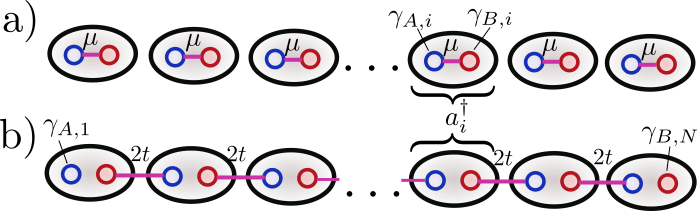
\includegraphics[scale=0.5]{IMAGES/Majorana/KitaevChain.png}
    \label{fig:top.phases kitaev}
    \caption{Illustration of the Kitaev chain for open boundary conditions in the Majorana representation. a)Represents the trivial case where the hopping and the superconducting term approaches to $0$. b) The non-trivial topological phase. The coupling is produced between Majoranas in different Dirac fermions \protect\Source{By the author} }
\end{figure}


\begin{enumerate}
\item{If $\super = t = 0, \mu <0$} Hamiltonian \eqref{eq:HamMajorana} becomes $\frac{-i\mu}{2} \sum_{j} \gammaA{j}\gammaB{j}$ which represents the coupling of the Majoranas in the same Dirac fermion. (See Figure \ref{fig:top.phases kitaev} (a))

\item{If $\super = t > 0, \mu =0$} the situation is much more interesting. The Hamiltonian \eqref{eq:HamMajorana} takes the form $H = 2ti\sum_{j} \gammaA{j}\gammaB{j+1}$. This implies that the coupling is performed between  Majoranas of different Dirac fermions leaving the edge Majorana operators ($\gammaA{1}$ and $\gammaB{N}$) uncoupled (See Figure \ref{fig:top.phases kitaev}b)). Note that these uncoupled Majorana fermions can be at any state without any  repercussion in the energy of the system. This explains the emergence of a  ground state localized at edges of the chain. 
\end{enumerate}

These two situations are representatives of two different phases. The trivial phase occurs for $\frac{\mu}{2t}>1$ and the non-trivial phase appears when $\frac{\mu}{2t}<1$ (See figure \ref{fig:KitaevSpec}). The mean characteristic of the non-trivial phase is the creation of an stable zero-mode. This zero-mode is generated by the  uncoupled Majorana fermions at the edges of the Kitaev chain.  \\



\begin{figure}[t]
    \centering
    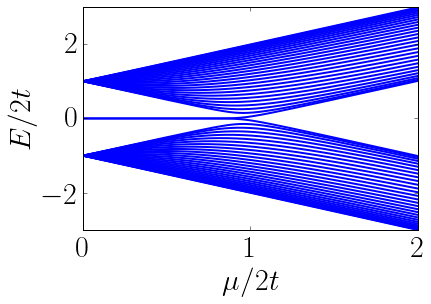
\includegraphics[scale=0.5]{IMAGES/Majorana/Spectrum.png}
    \label{fig:KitaevSpec}
    \caption{Spectrum of Hamiltonian \eqref{eq:HamMajorana} with $30$ sites and $t=\super$ s. Method: Numerical diagonalization. \protect \Source{By the author} }
\end{figure}



% ---------------Subsection: Topological phase transition-------------
\subsection{Topological phase transition}

The two regimes described previously  can be characterized with a topological parameter.  One of the methods for this is following the idea used by \citeauthor{alicea_new_2012}\cite{alicea_new_2012}. The first part is to suppose that we have an infinite chain $(N=\infty)$ in Hamiltonian \eqref{eq:HamMajorana}. The new system is translation invariant, hence we can make a transformation to the momentum space. Then we may rewrite Hamiltonian \eqref{eq:HamMajorana}  as

\begin{equation}
    H = 
    \sum_{k \in BZ} 
    \begin{pmatrix} 
      b_k'  & c_{k}'\\  
    \end{pmatrix}
    H_k 
    \begin{pmatrix} 
      b_{-k}'     \\ 
      c_{-k}' 
    \end{pmatrix}.
    \label{PBCHam2}
\end{equation}

with the Bloch Hamiltonian 

\begin{equation}
H_k = \begin{pmatrix} 
      0    &  \frac{-i \mu}{2} + it \cos k + \super  \sin k  \\ 
       \frac{i \mu}{2} - it \cos k + \super \sin k  &  0 
    \end{pmatrix}
    = (\super \sin k) \sigma_x + (\frac{\mu}{2}- t \cos k) \sigma_y.
\label{sigma}
\end{equation}




\noindent where $\sigma_x$ , $\sigma_y$ are the corresponding Pauli matrices. The Brilloin zone ($BZ$) is the periodic space  $[-\pi , \pi]$ which can be mapped to the unitary circle.   Equation \eqref{sigma} determines  the coordinates of the Bloch Hamiltonian in the base $\{\sigma_x, \sigma_y\}$. We can map these coordinates to the unitary circle by taking the norm of this vector giving
\begin{equation}
     \hat{H}_k= \frac{1}{\sqrt{\super^2 \sin^2 k + (\frac{\mu}{2}- t \cos k)^2}}
     \begin{pmatrix} 
      \super \sin k    \\ 
      \frac{\mu}{2}- t \cos k 
    \end{pmatrix}. 
\end{equation}

Note that $\super^2 \sin^2 k + (\frac{\mu}{2}- t \cos k)^2 \neq 0$ for all the values of $k$ as long as $\frac{\mu}{2t} \neq 1$ . When $\frac{\mu}{2t} = 1$ the $H_{k=0}=0$, so it cannot be normalized. \textbf{This is the same point were the phase transition occurs!}. At any other value of $\frac{\mu}{2t}$ it is possible to normalize $H_{k}$ for all values of $k\in BZ$. The result of mapping $\hat{H}_k$ for all $k$ is a path around the unitary circle. \\

This path can take two forms as we can observe in Figure \ref{fig:topological}. If $\frac{\mu}{2t} > 1$ the path reduced to a line in the upward part of the circle. In the non-trivial phase $\frac{\mu}{2t} < 1$ the path completes the round to the entire circle. Note that this method states a topological difference between the two phases. While the path described by the trivial phase can be contracted to a single dot, the path described by the non-trivial one is a circle that cannot be contracted. \\

Note that to determine whether path of a given phase is of type a) or type b) we only need to check if $\hat{H}_{k=0}$ and $\hat{H}_{k=\pi}$ are the same point or opposite points. This transforms into a simple equation 
\begin{equation}
    \hat{H}_{k=0,y}\hat{H}_{k=\pi,y}=\begin{cases}
1 & \mbox{trivial phase}\\
-1 & \mbox{non-trivial phase}
\end{cases}
\end{equation}
where $\hat{H}_{k=0,y}$ is the $y$-th component of $\hat{H}_{k}$. The term $\hat{H}_{k,y}$ is a particular case of the Pfaffian $\mathcal{P}(k)$, which widely used as topological order in  phases transition including  Majorana modes . 


\begin{figure}[t]
    \centering
    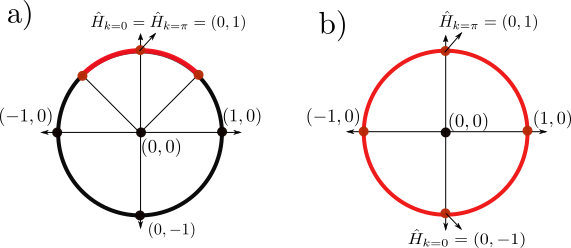
\includegraphics[scale=0.8]{IMAGES/Majorana/Topological.png}
    \label{fig:topological}
    \caption{ The following represents the path of $\hat{H}_k$ for the interval $[ -\pi, \pi ]$. a) Corresponds to the trivial phase. The resulting path can be homotopically deformed to a point. b) The non-trivial phase corresponds to a non-contractible loop around the unitary circle. \protect \Source{By the author}} 
\end{figure}

The mean idea behind this topological characterization relies in the adiabatic theorem.  In simple words, the adiabatic theorem says that a slow evolution of a gaped Hamiltonian will produce a smooth evolution of its ordered eigenstates. i.g The order of the eigenstates remains unchanged. \\

The keyword in the previous definition is "gaped". As we can observe in Figure \ref{fig:KitaevSpec} the phase transition occurs at $\frac{\mu}{2t}=1$. This is when the system transitions between a gapless and gaped Hamiltonians.  \\

The connection with topology comes from the fact that adiabatic evolutions can be understood as smooth deformations of the Hamiltonian. However since gapless Hamiltonians imply phase transitions, the theory defines the gapless points as holes (or forbidden points) in the phase space. Then characterizing the phase transitions in the Kitaev chain is mainly a topological problem where gaped Hamiltonians are holes in the topological space. In addition, the topological orders characterizing this transition will be Chern or Winding numbers. \\


% Though this connection between physics and topology is quite interesting, I will stop here because it is taking us out of our real discussion which is Majorana fermions.  You can find more information about this in ( \Jesus{add references}). 

% -----------------------Subsection: Non-abelian Statistics -------------
%\subsection{Non-abelian statistics}







% -----------------------Section: Modern and Experimental-------------
\section{Real implementations of Majorana Chains}
\Jesus{Here comes a summary of real models and implementations of Majorana chains. I am still thinking how to write this section. For now, I leave some ideas}

Although the Kitaev chain its just a toy model, 

The promise of finding the exotic Majorana particles that could bring new insights to quantum computing motivated the implementation of real models that could emulate the physics of a Kitaev chain. 

Spin is a major problem. A material with spin-orbit coupling is  the solution to this situation. \ref{fig:sipin-orbit} 

\begin{equation}
    H =\int\mbox{d}x\psi^{\dagger}\left(\frac{\partial^{2}}{2m\partial x^{2}}-\mu -i\alpha\sigma_{y}\partial x+h\sigma_{x}\right)\psi+\Delta\psi_{\downarrow}\psi_{\uparrow}+\Delta^{*}\psi_{\downarrow}\psi_{\uparrow},
    \label{eq:MajoranaChainHam}
\end{equation}




\begin{figure}[t]
\centering
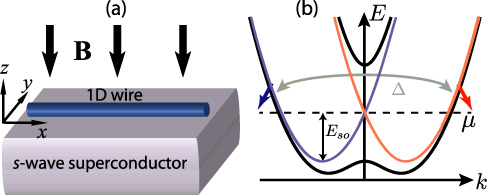
\includegraphics[scale=0.7]{IMAGES/Majorana/Mwire.png}

\caption{ \label{fig:spin-orbit} \protect\Source{\cite{alicea_new_2012}}}
\end{figure}

\begin{figure}[H]
\centering

     \subfloat[ \label{fig:exp1}]{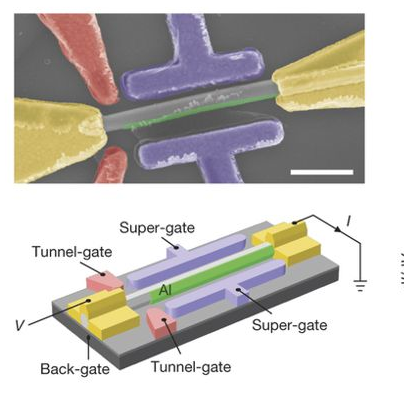
\includegraphics[scale=0.3]{IMAGES/Majorana/Exp.png}}  
     \subfloat[\label{fig:exp2}]{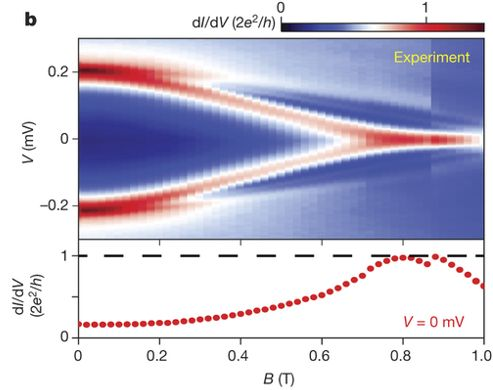
\includegraphics[scale=0.3]{IMAGES/Majorana/Exp2.png}}
\caption{ \label{ex}\protect\Source{\cite{zhang_quantized_2018}}}
\end{figure}


% -----------------------Leaking Majorana modes in quantum dots-------------

\section{Coupling Majorana Fermions to QDs}
\citeauthor{liu_detecting_2011} was one of the first to propose the possibility of using QDs in the pursuit of Majorana fermions . When a QD is attached to the end of a Majorana chain in the topological phase,  the Majorana Zero Mode at the end of the chain leaks inside the QD \cite{vernek_subtle_2014}. This produces a zero-bias conductance peak of half a quanta $\frac{e^{2}}{2h}$ through the dot. Using the ideas from \ref{chap: Methods} we can recreate this result. This will also allow us to probe our methods before going to the double-dot Majorana system in the following chapter. 

The Hamiltonian for Majorana-QD-lead hybrid system is is given by
\begin{equation}
    H=H_{QD-Lead}+H_{M-QD}+H_M.
\end{equation}
Where $H_{QD-Lead}$ is the Hamiltonian for the non-interacting Anderson model \eqref{eq:Anderson}, $H_M$ is the Hamiltonian of the Majorana chain and $H_{M-QD}$ represents the coupling between the QD and the Majorana Fermion at the boundary.

Now, the real question is how to define the coupling between the QD and the Majorana fermion. In fact, there are many ways to represent this interaction. One alternative is to replace in $H_{M}$ with the entire Kitaev chain hamiltonian \eqref{eq:kitaevHam} (or  even with the  Majorana chain \eqref{eq:MajoranaChainHam}) and then pick $H_{M-QD}$ as a simple coupling between the QD and the first site of the chain \cite{vernek_subtle_2014}.  A simpler approach is  to define an effective coupling with the Majorana operator at the edge of the Majorana chain. Since the Kitaev chain is spin-less, we choose to couple the Majorana to the spin-$\dw$ channel of the QD \footnote{An appropriate justification of this fact can be found in \cite{ruiz-tijerina_interaction_2015}} . Therefore, the Majorana fermion should be the superposition of the creation and annihilation operators of a spin $\dw$ particle $f_\dw$:

$$\gamma_1 := \frac{1}{\sqrt{2}} \left( f^\dagger_{\dw} + f_{\dw}\ \right) , \gamma_2 := \frac{1}{\sqrt{2}} \left( f^\dagger_{\dw} - f_{\dw} \right).$$

This makes possible to define an effective coupling between the Majorana Mode and the dot by attaching $\gamma_1$ with the spin-$\dw$ channel in the QD

%H_{TS} & = & 2\epsilon_{m}\gamma_{1}\gamma_{2}\nonumber \\
\begin{eqnarray}
H_{M-QD} & = &  t_1 \left(d_{\downarrow}^{\dagger}\gamma_{1}+\gamma_{1}d_{\downarrow}\right) 
% \\
% & = &  \sum_{i}t_{i} \left(d_{i\downarrow}^{\dagger}f^\dagger_{\dw} + 
% f_{\downarrow}d_{i\dw} +d_{i\downarrow}^{\dagger}f_{\dw}+
% +f_{\downarrow}^{\dagger} d_{i\downarrow}\right).
\label{eq:MajoranaCoupling}
\end{eqnarray}




% \begin{equation}
%     \omega\Green{A,B} =\delta_{A^{\dagger},B}+\Green{\left[A,H\right],B}
% \end{equation}

Then the coupling with the chain is given by 

\begin{eqnarray*}
H_{M} & = & \epsilon_{m}f_{\downarrow}^{\dagger}f_{\downarrow}\\
H_{M-QD}&=&\frac{t_1}{\sqrt{2}}d_{1\downarrow}^{\dagger}f_{\downarrow}+\frac{t_1^{*}}{\sqrt{2}}f_{\downarrow}^{\dagger}d_{1\downarrow}+\frac{t_1}{\sqrt{2}}d_{1\downarrow}^{\dagger}f_{\downarrow}^{\dagger}+\frac{t_1^{*}}{\sqrt{2}}f_{\downarrow}d_{1\downarrow}
\end{eqnarray*}

Finally we obtain the following hamiltonian

\begin{equation}
H =\sum_{k,\sigma}\left(\epsilon_1+\frac{U_1}{2}\right)d_{1\sigma}^{\dagger}d_{1\sigma}+ \frac{U}{2}(d_{1\sigma}^{\dagger}d_{1\sigma}-1)^{2} + t_1 \left(d_{1\downarrow}^{\dagger}\gamma_{1}+\gamma_{1}d_{1\downarrow}\right) + Vd^\dagger_{1\sigma}c_{k\sigma}+V^* c^\dagger_{k\sigma}d_{1\sigma}+ \epsilon_{m}f_{\downarrow}^{\dagger}f_{\downarrow}.
\label{eq:QD-Mham}
\end{equation}


The fidelity of this effective model has been discussed by \citet{ruiz-tijerina_interaction_2015}
concluding that the Majorana effective hamiltonian reproduces the
same results than the Kitaev chain model in the topological phase
(This statement is true even for more realistic models of the TS that
include Rashba spin-orbit interactions and a Zeeman field \citep{ruiz-tijerina_interaction_2015}
).\\


\subsection{Non-interacting QD coupled to a Majorana chain}

In the non-interacting case we can use the ballistic transport equations from \ref{sec:transport}.The green functions are then determined by the following set of linear equations. 




\begin{align}
    \left(\omega-\epsilon_{M}\right)\Green{f_{\downarrow},d_{1\downarrow}^{\dagger}}&=\left(\omega+\epsilon_{M}\right)\Green{f_{\downarrow}^{\dagger},d_{1\downarrow}^{\dagger}}=\frac{t^*_1}{\sqrt{2}}\left(\Green{d_{1\downarrow},d_{1\downarrow}^{\dagger}}-\Green{d_{1\downarrow}^{\dagger},d_{1\downarrow}^{\dagger}}\right)\\
    \left(\omega-\epsilon_{1}\right)\Green{d_{1\downarrow},d_{1\downarrow}^{\dagger}}&=1+\frac{t_1}{\sqrt{2}}t_{1}\Green{f_{\downarrow},d_{1\downarrow}^{\dagger}}+\frac{t_1}{\sqrt{2}}t_{1}\Green{f_{\downarrow}^{\dagger},d_{1\downarrow}^{\dagger}}+V_{1}\sum_{\mathbf{k}}\Green{c_{\mathbf{k\downarrow}},d_{1\downarrow}^{\dagger}}\\
    \left(\omega-\epsilon_{\mathbf{k}}\right)\Green{c_{\mathbf{k}},d_{1\downarrow}^{\dagger}}&=V_{1}^{*}\Green{d_{1\downarrow},d_{1\downarrow}^{\dagger}}\\
    \left(\omega+\epsilon_{1}\right)\Green{d_{1\downarrow}^{\dagger},d_{1\downarrow}^{\dagger}}&=-\frac{t_1}{\sqrt{2}}\Green{f_{\downarrow},d_{1\downarrow}^{\dagger}}-\frac{t_1}{\sqrt{2}}\Green{f_{\downarrow}^{\dagger},d_{1\downarrow}^{\dagger}}-V_{1}^{*}\sum_{\mathbf{k}}\Green{c_{\mathbf{k\downarrow}}^{\dagger},d_{1\downarrow}^{\dagger}}\\
    \left(\omega+\epsilon_{\mathbf{k}}\right)\Green{c^\dagger_{\mathbf{k}},d_{1\downarrow}^{\dagger}}&=-V_{1}^{*}\Green{d_{1\downarrow},d_{1\downarrow}^{\dagger}}
\end{align}

The graph representing these green functions is represented in \ref{fig:green-M-QD} a)  (Look \ref{sec:GraphMethod} for details). However using that $\left(\omega-\epsilon_{M}\right)\Green{f_{\downarrow},d_{1\downarrow}^{\dagger}}=\left(\omega+\epsilon_{M}\right)\Green{f_{\downarrow}^{\dagger},d_{1\downarrow}^{\dagger}}$ we can take
 $\Green{f_{\downarrow}^{\dagger},d_{1\downarrow}^{\dagger}}$ out of the equations getting the system in \ref{fig:green-M-QD} b) .  Using the graph algorithm from \ref{sec:Algorithm}  we proceed to pop out vertexes $c_k$ , $c_k^\dagger$ and $d_1^\dagger$ in that order. The result is the graph in figure \ref{fig:green-M-QD}.c) with 
 
 \begin{figure}[t]
    \centering
    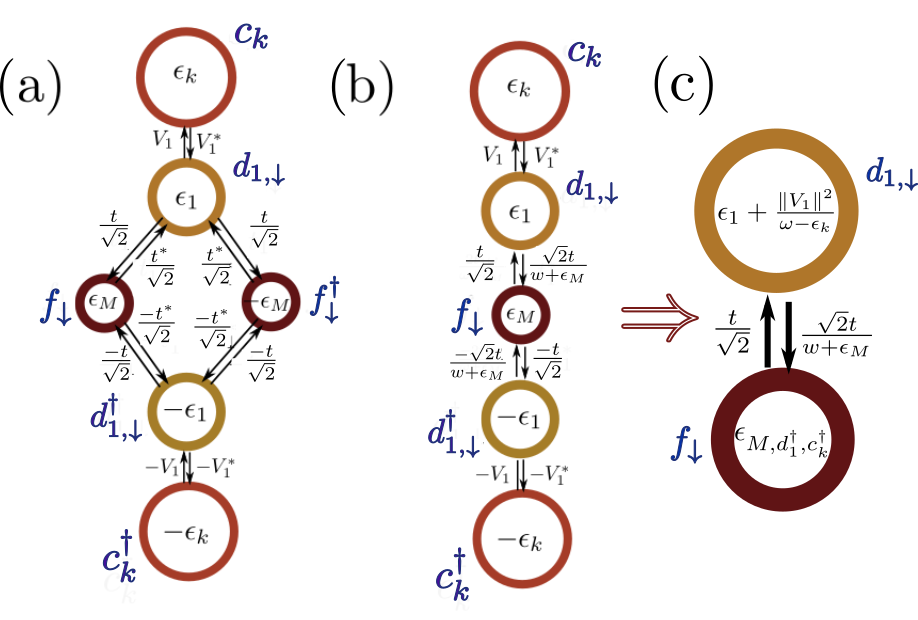
\includegraphics[scale=0.5]{IMAGES/Graphs/Grenn-Majorana.png}
    \caption{ Graph $\GM$ representing the transport equations.  \label{fig:green-M-QD} \protect\Source{By the author}}
\end{figure}
 
 \begin{equation}
    \epsilon_{M,d_1^\dagger,c^\dagger}= \epsilon_{M}+\frac{\omega}{\omega+\epsilon_{M}}\frac{\left\Vert t\right\Vert ^{2}}{\omega+\epsilon_{1}+\sum_{\mathbf{k}}\frac{V_{1}V_{1}^{*}}{\omega+\epsilon_{\mathbf{k}}}}.
\end{equation}
 
 We finally pop out $f_\dw$ to obtain 
 
\begin{equation}
    \Green{d_{1\downarrow},d_{1\downarrow}^{\dagger}}=\left[\omega-\epsilon_{1}-\sum_{\mathbf{k}}\frac{V_{1}V_{1}^{*}}{\omega-\epsilon_{1}}-\frac{\omega}{\omega+\epsilon_{M}}\frac{\left\Vert t\right\Vert ^{2}}{\omega -\epsilon_{M,d_1^\dagger,c^\dagger}}\right]^{-1}.
\end{equation}
Hence we just need the green function of $\GreenG{f_{\downarrow},f_{\downarrow}^{\dagger}}{\GM-d_{1}}$ removing $d_1$ out of the graph. This case is much simpler since $f_\downarrow$ is just attached to $d^\dagger_1$ . Thus we get
\begin{equation}
    \GreenG{f_{\downarrow},f_{\downarrow}^{\dagger}}{\GM-d_{1}}=\left[\omega-\epsilon_{M}-\frac{\omega}{\omega+\epsilon_{M}}\frac{\left\Vert t\right\Vert ^{2}}{\omega+\epsilon_{1}-\sum_{\mathbf{k}}\frac{V_{1}V_{1}^{*}}{\omega-\epsilon_{\mathbf{k}}}}\right]^{-1}.
\end{equation}

The only missing point in this equation is to replace $\sum \frac{V_1V^*_1}{\omega -\epsilon_k}= -i\Gamma_1$ as we already did in \ref{sec:GraphMethod}. Note that these computations are only for the spin-$\dw$ channel. The spin-$\up$ channel is even simpler since this channel is not coupled to the Majorana mode by convention. Hence it corresponds to the case of a single quantum dot coupled to a Lead.  The results for the DOS can be observed in \ref{fig:M1-Tot}. Each figure has an inset showing the model in the Majorana representation. The small blue and red balls are Majorana fermions just as the ones in figure \ref{fig:top.phases kitaev}. The Majorana at the edge of the  chain is represented by the isolated red ball connected to the QD (Figure \ref{fig:M1}). The other isolated blue ball in Figure \ref{fig:M1-em} represents the Majorana at the other edge which is connected to the sphere by the parameter $\epsilon$. 
\Jesus{Here comes the interpretation}
\begin{itemize}
    \item\textbf{Figure: \ref{fig:M1}}  The spin-$\up$ DOS shows the result when the Majorana is uncoupled, hence corresponding to a quantum dot coupled to a lead. When the Majorana is attached to the dot $t>0$ the DOS decays to the half. This robust signature 
    \item\textbf{Figure: \ref{fig:M1-e1}}
    \item\textbf{Figure: \ref{fig:M1-em}}
\end{itemize}



\begin{figure}[t]
     \centering
    \subfloat[Figure  \label{fig:M1}]{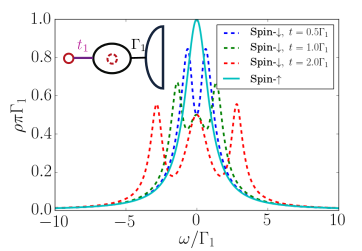
\includegraphics[scale=0.6]{IMAGES/Majorana/M1.png}}
     \subfloat[Figure \label{fig:M1-e1}]{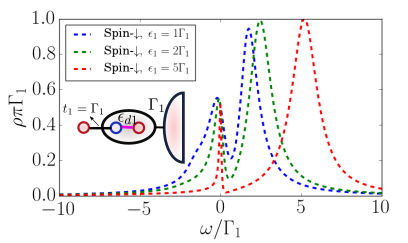
\includegraphics[scale=0.6]{IMAGES/Majorana/M1-e1.png}}  \\
    \subfloat[\label{fig:M1-em}]{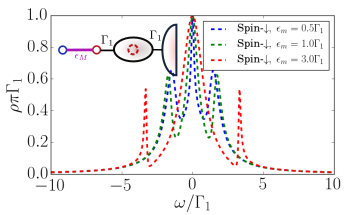
\includegraphics[scale=0.6]{IMAGES/Majorana/M1-eM.png}}
    
     \caption{Figure \label{fig:M1-Tot} ..\Jesus{I don't like the variables of  the c) plot. So I might change them soon}.  \protect\Source{ By the Author  }}
\end{figure}




\subsection{NRG: Kondo-Majorana physics}
In the interacting case the Kondo peak will appear at the fermi energy. In addition, the Majorana in the spin-$\dw$ channel will produce a peak at the fermi energy of Half of the amplitude of the Kondo peak (See \ref{fig:NRG-1M}). This will be our Majorana signature. 
\begin{figure}[H]
\centering
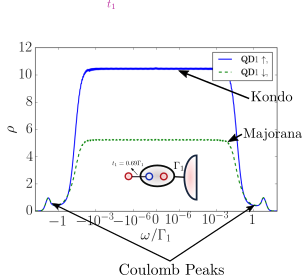
\includegraphics[scale=0.7]{IMAGES/Majorana/NRG.png}

\caption{ \Jesus{The units of this plot are a bit different than the NRG plots. That's mainly due to a problem I am having with the NRG plots. I will unify the format soon. } \label{fig:NRG-1M} \protect\Source{\cite{By the author.}}}
\end{figure}


 \citeauthor{ruiz-tijerina_interaction_2015}  proved that this effective coupling  is able to reproduce efficiently the results obtained when the Kitaev chain in the topological phase is attached to a single QD. 

% \begin{eqnarray*}
% H_{TS} & = & 2\epsilon_{m}f_{\downarrow}^{\dagger}f_{\downarrow}-\epsilon_{m}\\
% H_{int} & = & \sum_{i}\tilde{t_{i-}}d_{i\downarrow}^{\dagger}f_{\downarrow}+\tilde{t_{i-}}^{*}f_{\downarrow}^{\dagger}d_{i\downarrow}+\tilde{t_{i+}}d_{i\downarrow}^{\dagger}f_{\downarrow}^{\dagger}+\tilde{t_{i+}}^{*}f_{\downarrow}d_{i\downarrow}
% \end{eqnarray*}

% with $\tilde{t}_{i\pm}=\frac{1}{\sqrt{2}}\left(\left|t_{i1}\right|-i\left|t_{i1}\right|e^{i\phi_{i}}\right).$



% so that 

% \[
% \gamma_{1}=\frac{1}{\sqrt{2}}\left(f_{\downarrow}^{\dagger}+f_{\downarrow}\right)\ ,\gamma_{2}=\frac{1}{i\sqrt{2}}\left(f_{\downarrow}^{\dagger}-f_{\downarrow}\right).
% \]


% \begin{eqnarray}
% H_{TS} & = & 2\epsilon_{m}\gamma_{1}\gamma_{2}\nonumber \\
% H_{int} & = & \sum_{i}t_{i1}\left(d_{i\downarrow}^{\dagger}\gamma_{1}+\gamma_{1}d_{i\downarrow}\right)+it_{i2}\left(d_{i\downarrow}^{\dagger}\gamma_{2}+\gamma_{2}d_{i\downarrow}\right),\label{eq:Majorana-ham}
% \end{eqnarray}


% where $\gamma_{1,2}$are the two Majorana operators and$t_{i1,2}$
% are the hopping terms between the Majoranas and the QDs.




% A Majorana chain coupled to a QD can be studied using the methods described in chapter \ref{chap: Methods}






% % where $H_{d_{i}}$is the QD hamiltonian for dot $i$ \prettyref{eq:DotHam}
% % ,$t$ is the hopping term between both dots, $H_{int}$is the dot-TS
% % interaction and $H_{TS}$ is the TS-hamiltonian . In \citep{vernek_subtle_2014},
% % the TS is modeled as a Kitaev chain \citep{kitaev_unpaired_2001}
% % and $H_{int}$ is the hopping interaction between dots and chain 

% \begin{eqnarray}
% H_{TS} & = & -\sum_{j=1}^{N}\mu a_{j}^{\dagger}a_{j}+\sum_{j=1}^{N-1}\left[-t'(a_{j}^{\dagger}a_{i+1}+a_{j+1}^{\dagger}a_{j})+\Delta a_{j}a_{j+1}+\Delta^{*}a_{j+1}^{\dagger}a_{j}^{\dagger}\right]\nonumber \\
% H_{int} & = & \sum t_{i}d_{i\downarrow}^{\dagger}a_{1}+t_{i}^{*}a_{1}^{\dagger}d_{i\downarrow},\label{eq:Kitaev-dot}
% \end{eqnarray}


% where $a_{j}^{\dagger}$is the creation operator at site $j$ of the
% chain, $t'$ is the hopping term between consecutive sites, $\Delta$
% is the superconducting gap and $t_{i}$ is the hopping interaction
% between the dot $i$ and the first site of the chain. We also assume
% the dot only interact with spin-down $\downarrow$ operators in the
% chain. \\

% Using a Green's function approach on \prettyref{eq:Kitaev-dot} ,
% \citet{vernek_subtle_2014} concludes that the Majorana mode at the
% end of the chain leaks inside the QD when the TS is in the topological
% phase . This fact favors a more simple effective model that has been
% used in literature for simulation QD-TS interactions \citep{liu_detecting_2011,golub_kondo_2011,lee_kondo_2013}.
% The model consists in considering only the coupling between the dots
% and the Majorana modes that emerge in the topological phase. The resulting
% hamiltonian is 



% \[
% f_{\downarrow}^{\dagger}=\frac{1}{\sqrt{2}}\left(\gamma_{1}-i\gamma_{2}\right)\ ,\ f_{\downarrow}=\frac{1}{\sqrt{2}}\left(\gamma_{1}+i\gamma_{2}\right)
% \]


% so that 

% \[
% \gamma_{1}=\frac{1}{\sqrt{2}}\left(f_{\downarrow}^{\dagger}+f_{\downarrow}\right)\ ,\gamma_{2}=\frac{1}{i\sqrt{2}}\left(f_{\downarrow}^{\dagger}-f_{\downarrow}\right).
% \]


% Supposing $t_{i1}=\left|t_{i1}\right|$ and $t_{i2}=\left|t_{i2}\right|e^{i\phi_{i}}$
% to have a $\phi_{i}$-phase with respect to $t_{i1}$, we get to the
% following hamiltonian 



% \begin{eqnarray}
% H_{TS-2QDs} & = & H_{d_{i}}+\sum_{\sigma}\left(td_{1\sigma}^{\dagger}d_{2\sigma}+t^{*}d_{1\sigma}^{\dagger}d_{2\sigma}\right)\nonumber \\
%  &  & \ \enskip\ \enskip+\sum_{i}\left[\tilde{t_{i-}}d_{i\downarrow}^{\dagger}f_{\downarrow}+\tilde{t_{i-}}^{*}f_{\downarrow}^{\dagger}d_{i\downarrow}+\tilde{t_{i+}}d_{i\downarrow}^{\dagger}f_{\downarrow}^{\dagger}+\tilde{t_{i+}}^{*}f_{\downarrow}d_{i\downarrow}\right]+2\epsilon_{m}f_{\downarrow}^{\dagger}f_{\downarrow}-\epsilon_{m}.\label{eqFinalMJ-2QDs}
% \end{eqnarray}



% \chapter{Coupling a Double Quantum Dot with a Majoran Mode}
%--------------------------------------------------------------------------
\note{This section is still a bit disorganized since most of the results are new.   }
In this section we present the results for the NRG analysis of the Anderson model applied to the case of a Double Quantum Dot (DQD) attached to a Majorana mode (See \ref{fig:GeneralModel}). Extending the  Hamiltonian \eqref{eq:QD-Mham} to a coupling with a DQD we obtain the following general Hamiltonian:   

\begin{equation}
H =\sum_{i=1}^2\sum_{k,\sigma}\left(\epsilon_{i}+\frac{U_i}{2}\right)d_{\sigma}^{\dagger}d_{i\sigma}+ \frac{U_i}{2}(d_{i \sigma}^{\dagger}d_{i \sigma}-1)^{2} + t_i(\gamma d_{+,\dw}+d^\dagger_{+,\dw}\gamma) + V_id^\dagger_{i\sigma}c_{k\sigma}+V_i^* c^\dagger_{k\sigma}d_{i\sigma}.
\label{General model}
\end{equation}

\Jesus{I neglected $\epsilon_M$ in this case. Depending on the future NRG results I will choose to add it or leave it that way. }


\begin{figure*}[h]
\centering
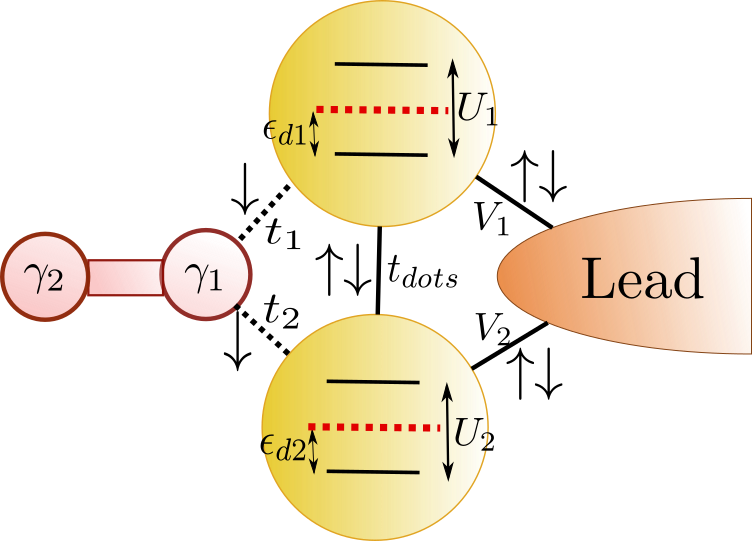
\includegraphics[scale=0.4]{IMAGES/GenModel.png}
\caption{\label{fig:GeneralModel}General model.} 
\end{figure*}



In order to understand the physical properties of this model, we probed a set of thought processes. The main variable in this analysis is the Density of States.  We  will observe its evolution on both QDs under the tuning of the model parameters such as:
\begin{enumerate}
    \item Hopping between Dots and Majorana Mode ($t_1 , t_2$). 
    \item Gate voltage ($\ed{1} , \ed{2} $)
    \item Inter dot coupling ($t_{dots}$)
\end{enumerate}


These processes intend to show whether it is possible to "manipulate" the majorana modes inside the dots by tuning the established parameters.The processes we found to show interesting physics are summarized in table. 
\begin{figure*}[h]
\centering
\includegraphics[scale=0.4]{IMAGES/Mo}
\caption{\label{fig:GeneralModel}General model.} 
\end{figure*}

\begin{figure*}[h]
\centering
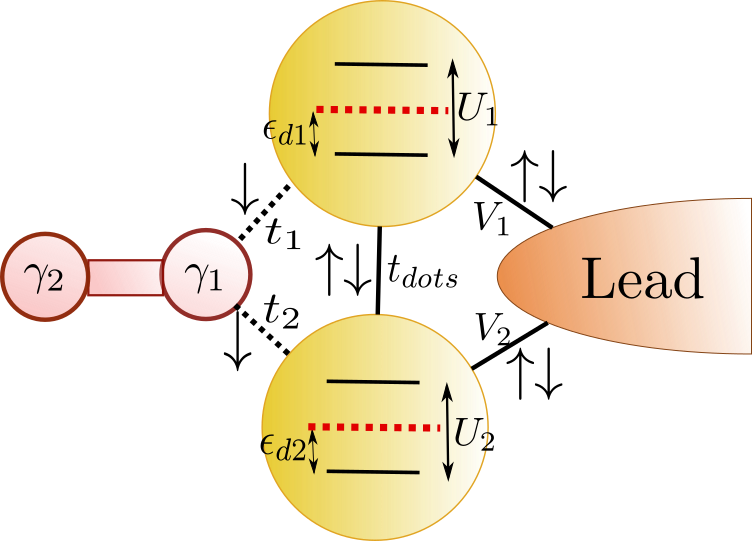
\includegraphics[scale=0.4]{IMAGES/GenModel.png}
\caption{\label{fig:GeneralModel}General model.} 
\end{figure*}


\newpage
\newpage



\section{Attaching the Majorana mode to the DQD (Tuning $t_1=t_2$) \label{sec:t1=t2}}

\textbf{Parameters:}

$$\Gamma \sim 2.83*10^{-2}D, t_{dots}=0 , U_{1,2} = -2\ed{1,2} = 0.5$$
$$t_1=t_2 \in [0\  ,\  2.5*10^{-2}D]$$

\begin{figure}[hbt]
\centering
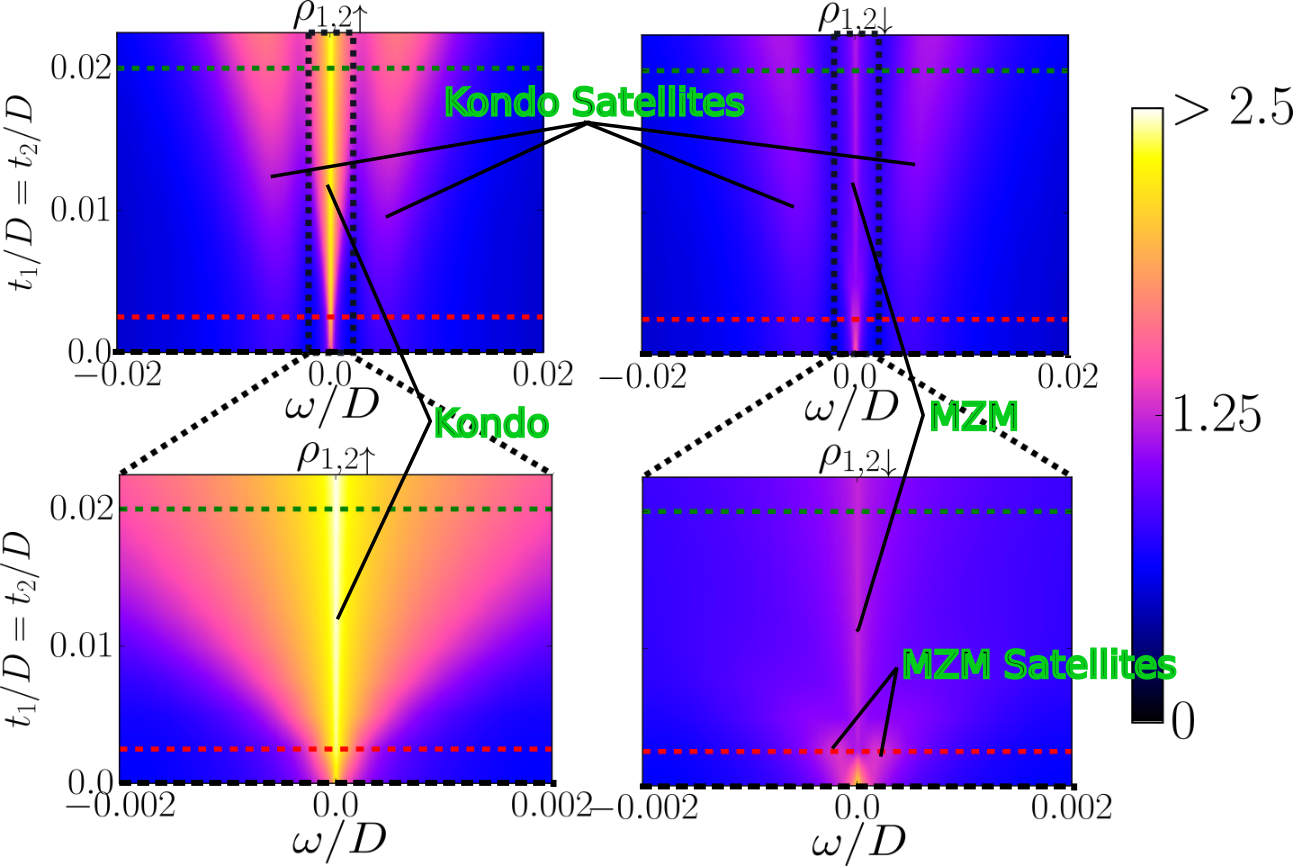
\includegraphics[scale=0.35]{IMAGES/t1=t2/2D.png}
\caption{\label{fig:2D/Shift_t1=t2} Evolution of the DOS of both QDs through $t_1 = t_2$ tuning. UP: Energy scale $\omega \sim 10^{-2}D$. DOWN: Energy scale $\omega \sim 10^{-3}D$. LEFT: Spin $\up$. RIGHT: Spin $\dw$.}
\end{figure}



The first process consists in attaching the Majorana mode to both Quantum Dots symmetrically. For this, we scale up the coupling parameter $t_1=t_2$ from $0$ (Decoupled) to $0.02$ (Completely coupled).The other parameters where chosen with an equilibrium between the dot energy and Coulomb repulsion $(\ed{1,2}=-\frac{U_{1,2}}{2})$  and  without inter-dot coupling $t_{dots}=0$. These circumstances guarantee that the system preserves Particle Hole Symmetry (PHS). Thus the Density of States (DOS) of particles and holes remains equal at all instances $(\rho(-\omega) = \rho(\omega))$. \\

\begin{figure}[hbt]
\centering
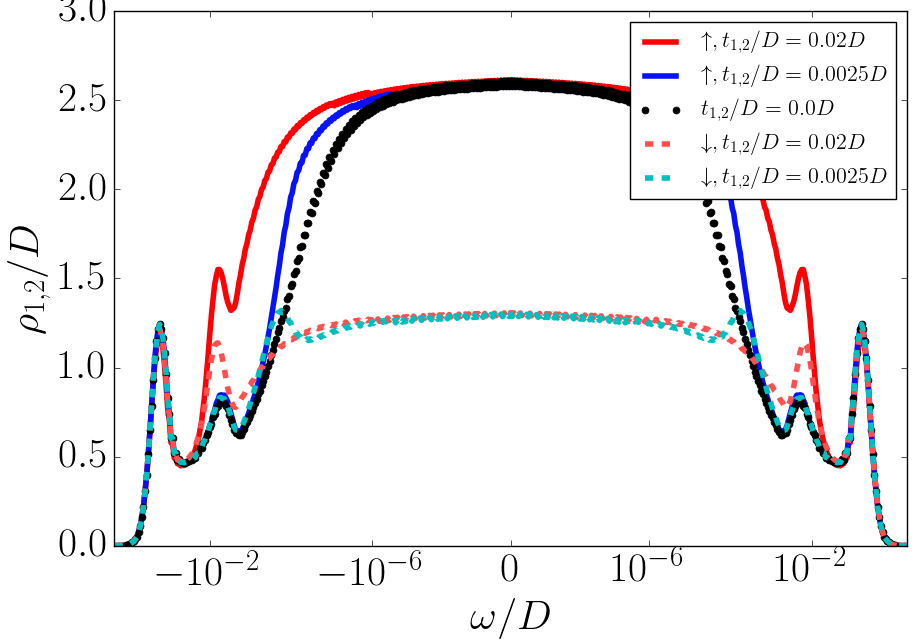
\includegraphics[scale=0.35]{IMAGES/t1=t2/LogPlot.png}
\caption{\label{fig:t1=t2/logplot} Density of states at each QD of the horizontal dashed cuts in \ref{fig:2D/Shift_t1=t2}. The energy is in logarithmic scale.  For $t_1=t_2>0$ spin-$\up$ and spin-$\dw$ DOS split near the order of $\vert \omega \vert \sim t_1,2 $. At the Fermi energy $(\omega =0)$  $\rho_\up = 2\rho_\dw$ due to the presence of the MZM in both QDs. }
\end{figure}

In the case where the majorana is detached from the DQD $(t_1 =t_2 = 0)$, the system favors the appearance of a three-peak at low energies as it is shown in \ref{fig:t1=t2/logplot} . The central peak is produced only by the Kondo effect and the two other satellite peaks are the result of a strong correlation between both dots caused by the indirect exchange of quantum states through the Lead \ref{sec:DoublePeak}. \\

Once the MZM the spin-$\up$ and spin-$\dw$ DOS split at low energies due to the new spin-$\dw$ transport channel through the Majorana mode. The spin-$\dw$ DOS at the Fermi energy ($\omega =0$) decays to the half of the spin-$\up$ DOS $\rho_\dw = \frac{\rho_\up}{2} $. By symmetry in the dot parameters this event occurs equally for both QDs. We adopt this fact as a Majorana signature. Hence we obtain that the MZM leaks inside both quantum dots. 

There is also an additional effect caused by the indirect exchange between the QDs through the Majorana mode . The consequences of this effect depend on the energy range of the majorana couplings $t_1=t_2$.  : 
\begin{enumerate}
    \item If $t_1=t_2 \ll \Gamma $ two more satellites are formed at very low energies ($\sim t_1$) in the spin-$\dw$ DOS (See  \ref{fig:2D/Shift_t1=t2} Spin-down $\omega \sim 10^{-3}D$ ). (See  \ref{fig:2D/Shift_t1=t2} Spin $\up$, $\omega \sim 10^{-3}D$ ).
    \item If $t_1=t_2 \sim \Gamma$ , the MZM contributes to the the growth of the spin-up satellites in the DOS. This effect produces the splitting between the spin-up and spin-down DOS.   (See  \ref{fig:2D/Shift_t1=t2} Spin-$\dw$, $\omega \sim 10^{-2}D$).
\end{enumerate}








\iffalse
At low energies $(\omega/D \sim 10^{-2})$ \ref{fig:2D/Shift_t1=t2} shows the emergence of a 3-peak in the DOS close to the Fermi energy. This 3-peak is formed by a central peak defined by the Kondo (spin $\up$) and the Majorana (spin $\dw$) peaks. The other two peaks are generated by an indirect exchange of the states between the quantum dots through the leads (SEE ABSTRACT). At even lower energies $(\omega/D \sim 10^{-4})$ it is possible to appreciate the emergence of another 3-peak in the spin down DOS which is present only for small values of the Majorana coupling constants $t_1 = t_2 \ll 0.01D$ (See  \ref{fig:t1=t2/logplot}). These sided peaks are caused by the indirect exchange between both dots through the Majorana Mode. When the Majorana couplings achieve the same order of the dot-lead coupling $\Gamma$ $(t_1 = t_2 \sim  0.01D)$ both sided peaks are merged causing the extinction of the majorana side-peaks and the increase of the indirect exchange peaks at $(\omega/D \sim 10^{-2})$. 

\begin{figure}[H]
\centering
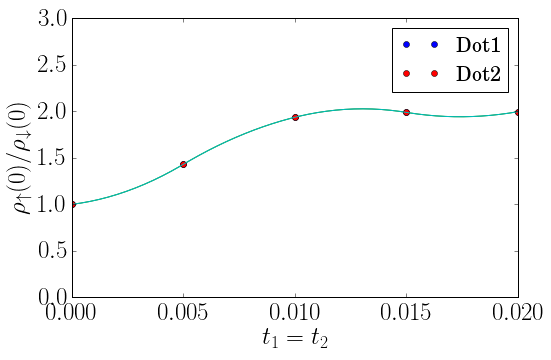
\includegraphics[scale=0.4]{Plots/MSig/Shift_t1=t2.png}
\caption{\label{fig:MSig/Shift_t1=t2} Relation between the Zero-peaks at the fermi level. The Majorana signature is related to $\frac{\rho_\up(0)}{\rho_\up(0)}=2$.}
\end{figure}
\fi




















%--------------------------------------------------------------------

\section{Transferring the MZM through gate voltage shifting $\ed{2}$. \label{sec:e2}}

\textbf{Parameters:}

$$\Gamma \sim 2.83*10^{-2}D, t_{dots}=0 , U_{1,2} = -2\ed{1} = 0.5 , t_1=t_2=0.0025$$
$$\ed{2} \in [-0.25 \  , -0.05]$$

This process starts with the DQD coupled symmetrically  to the Majorana mode, just as in \ref{sec:t1=t2}. The idea of this process is to break PHS by increasing the energy of the second QD $\ed{2}$. This procedure should induce the Majorana to tunnel only into the first dot. 


\begin{figure}[h]
\centering
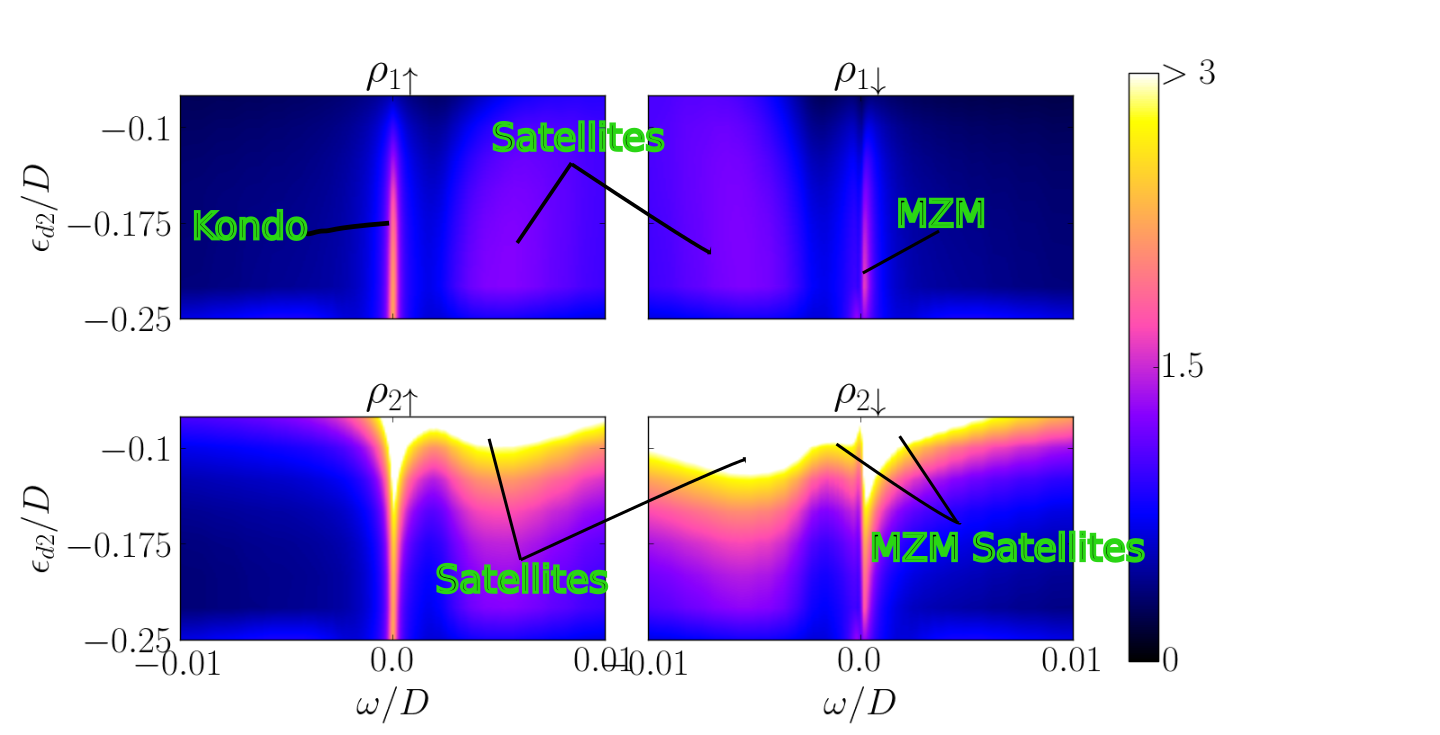
\includegraphics[scale=0.35]{IMAGES/ed2/2D.png}
\caption{\label{fig:2D/Shift_ed2} Evolution of the DOS of both QDs through the $\ed{2}$ tuning. UP: QD1. DOWN: QD2. LEFT: Spin $\up$. RIGHT: Spin $\dw$.}
\end{figure}


In \ref{fig:2D/Shift_ed2} we observe that both, the Kondo and the MZM peaks are preserved in the first QD as well as the majorana signature (See \ref{fig:ed2/Fermi}) when $\ed{2}$ is scaled up to $-0.1$.  However,  PHS breaking will favor the growth of the spin-$\up$ hole $(w>0)$  satellite and the spin-$\dw$ particle $(w<0)$ satellite.




In the second QD the DOS increases abruptly for both spins.The majorana signature is rapidly when  lost . Hence, with this set-up it is actually possible to induce the Majorana to preferably tunnel QD1 in despite of QD2.  \\
\begin{figure}[H]
\centering
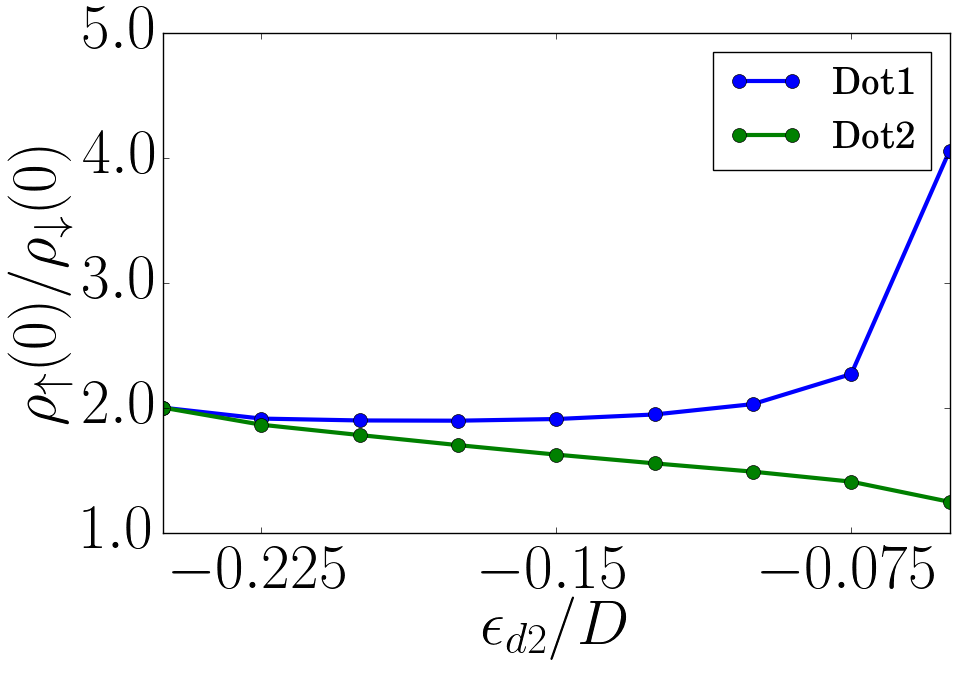
\includegraphics[scale=0.3]{IMAGES/ed2/Fermi.png}
\caption{\label{fig:ed2/Fermi} As described in \ref{sec:t1=t2} the relation $\frac{\rho_\up(0)}{\rho_\up(0)}=2$ constitutes a Majorana Signature . This picture evaluates shows the evolution of the relation $\frac{\rho_\up(0)}{\rho_\up(0)}$ for both QDs. While QD2 losses rapidly the Majorana signature, QD1 maintains it till $\ed{2}\sim -0.1$.}
\end{figure}


\newpage


%---------------------------------------------------------------------------

\section{Particle-Hole symmetric shifting of $\ed{2}=\frac{U}{2}$.}

\begin{figure*}[h]
\centering
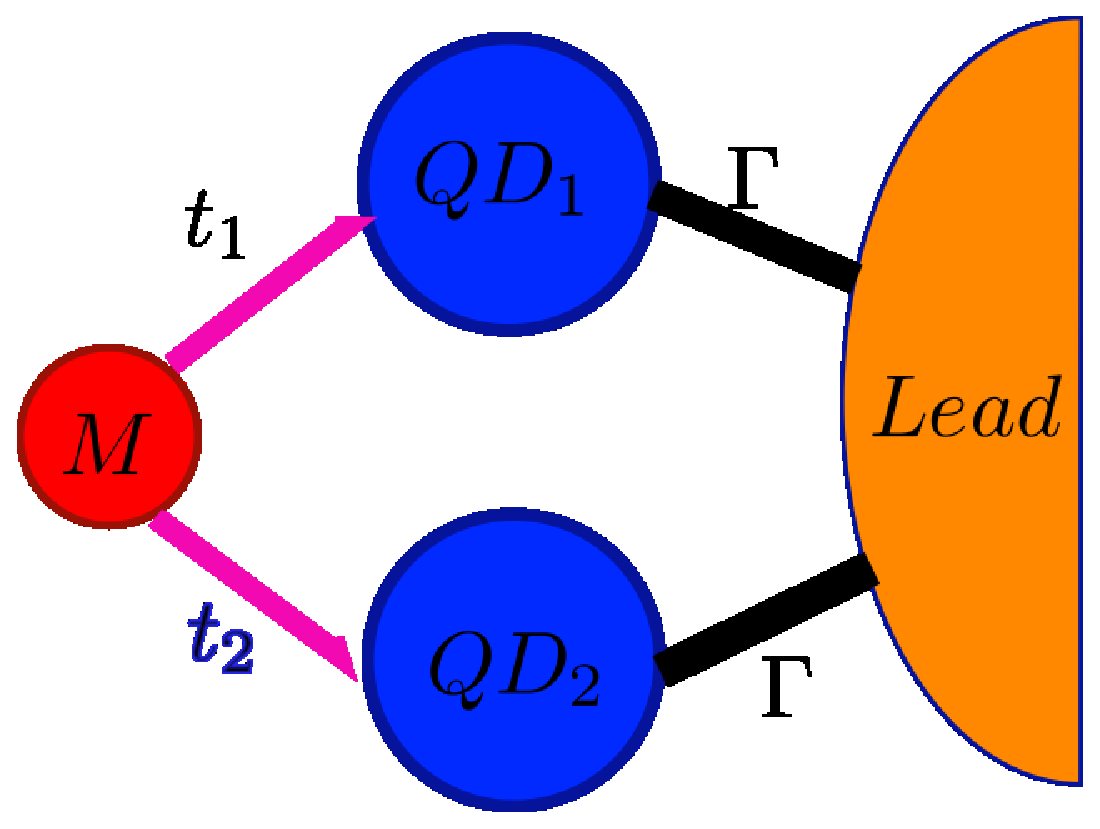
\includegraphics[scale=0.2]{Plots/Model/Majorana-2QD.eps}
\caption{\label{fig:Mod/PHS-Shift_e2.png}$U_{1}=-2\ep_{d1}=0.5$, $\Gamma_{1}=\Gamma_{2}$,
$t_{1}=t_2=0.02$. Variable $\ep_{d2} =\frac{U_{2}}{2}$}
\end{figure*}
\begin{figure}[hbt]
\centering
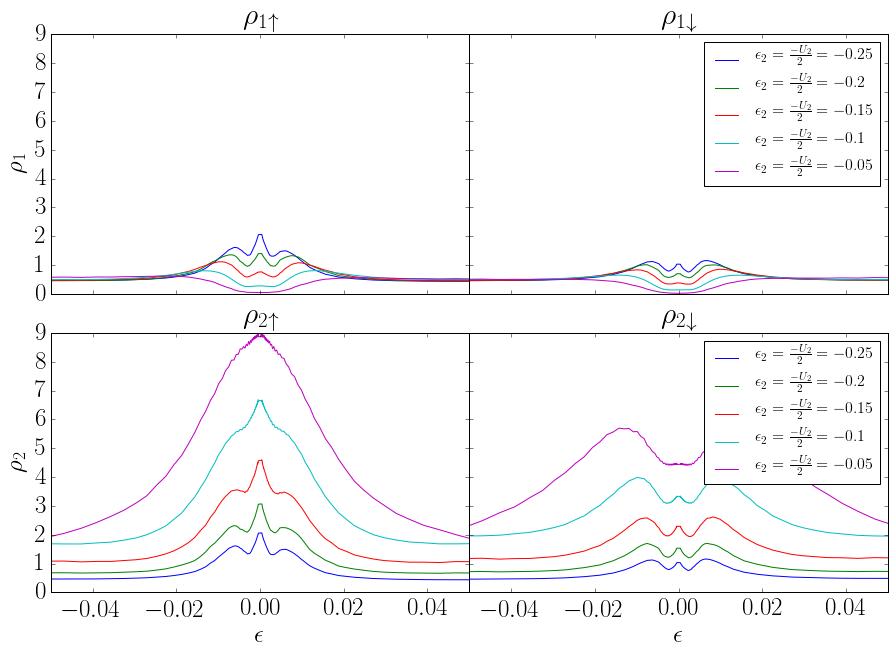
\includegraphics[scale=0.38]{Plots/DOS/PHS-Shift_e2.png}
\caption{\label{fig:DOS/PHS-Shift_e2.png} Evolution of the QDs' DOS for the model in \ref{fig:Mod/PHS-Shift_e2.png} }
\end{figure}
We start again with the symmetric model with both QDs coupled to the Majorana mode, but this time the evolution is performed over $\ep_2=\frac{U}{2}$, such that the model is always Particle-Hole symmetric. This situation is very different from the previous model (\ref{sec:e2}) since the decaying of $U2$ 
equalizes the effect of increasing the dot energy. In \ref{fig:DOS/PHS-Shift_e2.png} we observe that the DOS of QD2 increases while the QD1's DOS decreases, just as it happened in \ref{sec:e2} . However, the Majorana signature remains at $2$ for both dots (See \ref{fig:MSig/PHS-Shift_e2}), meaning that the Majorana is not preferably induced to tunnel to any QD despite the lose of symmetry in the dot energy.

\begin{figure}[hbt]
\centering
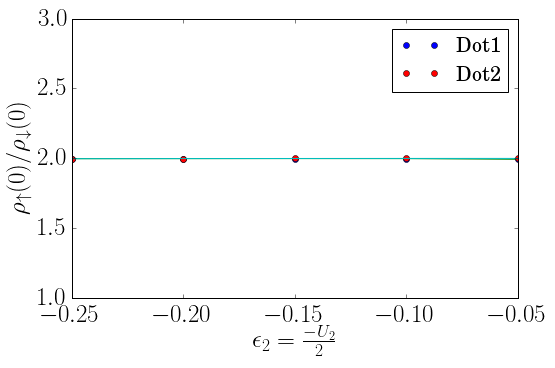
\includegraphics[scale=0.4]{Plots/MSig/PHS-Shift_e2.png}
\caption{\label{fig:MSig/PHS-Shift_e2} Relation between the spin up-down Zero-peaks at the Fermi level. The Majorana signature is related to $\frac{\rho_\up(0)}{\rho_\up(0)}=2$.}
\end{figure}

%---------------------------------------------------------------------------
\section{Shifting $t_2$}

%$U_{1}=U_{2}=-2\epsilon_{d1}=-2\epsilon_{d2}=0.5$, %$\Gamma_{1}=\Gamma_{2}$,
%$t_{1}=0.02$

\begin{figure*}[h]
\centering
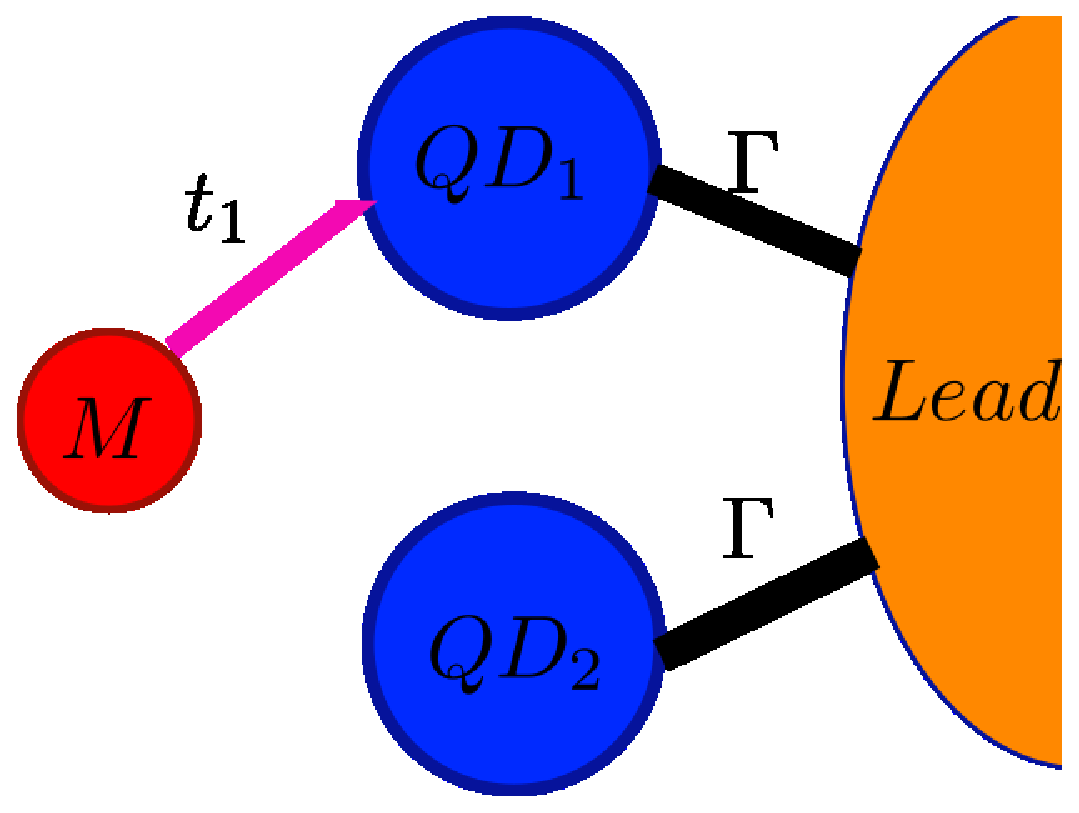
\includegraphics[scale=0.2]{Plots/Model/Majorana-1QD.eps}
\caption{\label{fig:Mod/Shift_t2}$U_{1}=U_{2}=-2\ep_{d1}=-2\epsilon_{d2}=0.5$, $\Gamma_{1}=\Gamma_{2}$,
$t_{1}=0.02$. Variable $t_2$}
\end{figure*}


\begin{figure}[hbt]
\centering
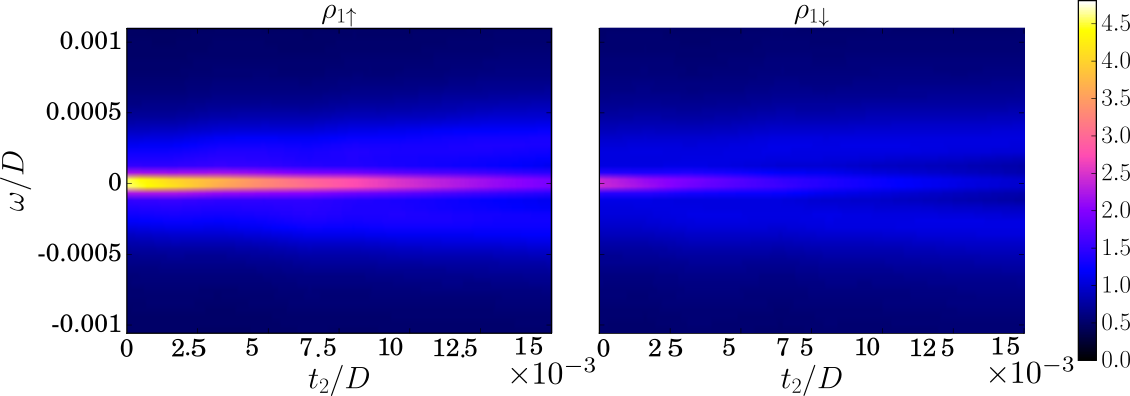
\includegraphics[scale=0.38]{Plots/2D/Shift_t2D1.png}
\caption{\label{fig:DOS/Shift_t2D1} Evolution of the DOS in the first QD }
\end{figure}
\begin{figure}[hbt]
\centering
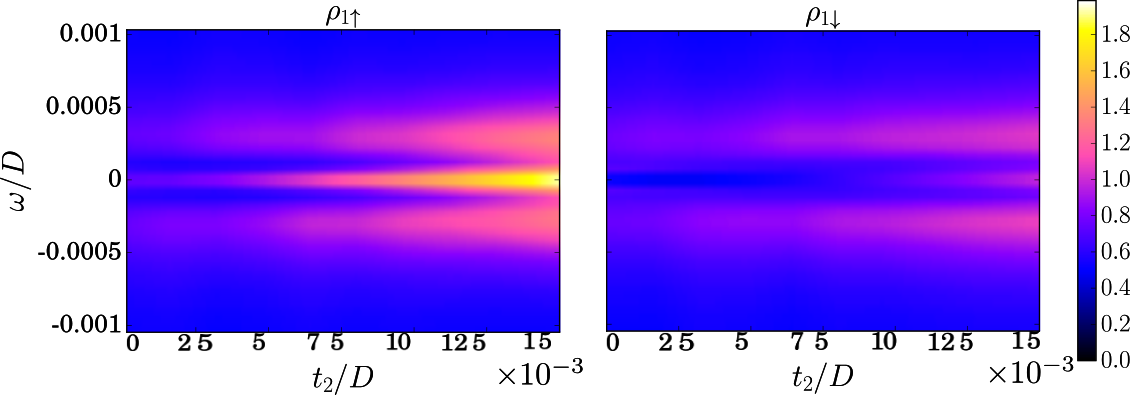
\includegraphics[scale=0.38]{Plots/2D/Shift_t2D2.png}
\caption{\label{fig:DOS/Shift_t2D2} Evolution of the DOS in the Second QD}
\end{figure}



\iffalse
\begin{figure}[hbt]
\centering
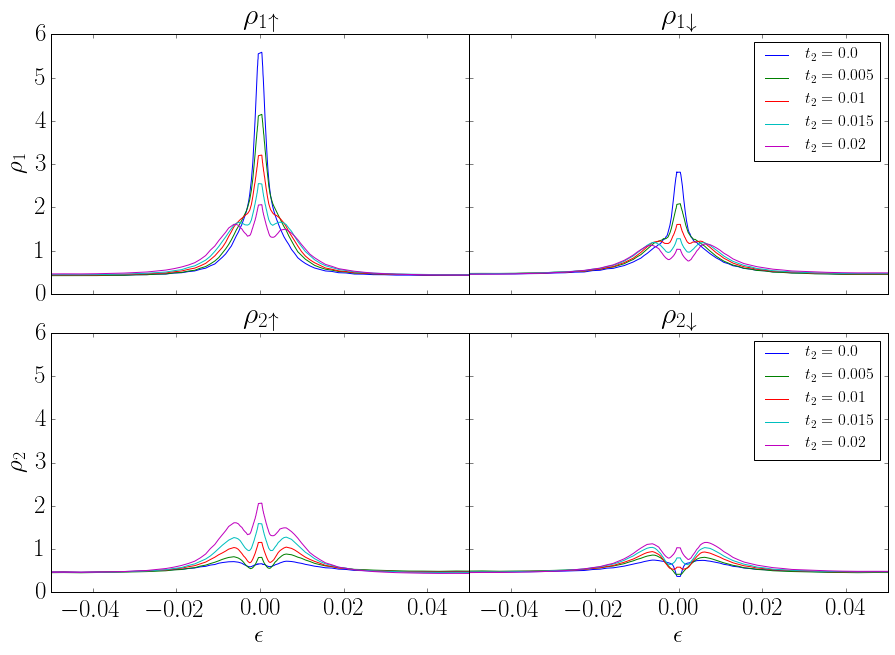
\includegraphics[scale=0.38]{Plots/DOS/Shift_t2.png}
\caption{\label{fig:DOS/Shift_t2} Evolution of the QDs' DOS for the procedure in \ref{fig:Mod/Shift_t2} }
\end{figure}
\fi
 In \ref{fig:DOS/Shift_t2D1} and \ref{fig:DOS/Shift_t2D1} we observe the evolution of DOS in the case where the second dot is smoothly connected to the Majorana, which is already attached to the first dot. The hopping parameter $t_2$ scales up to $0.015D$ where the model reaches the symmetry $t_2 = t_1$. The figures show that increasing $t_2$ leads to a drop in the DOS of QD1 while the DOS in QD2 is increased. In addition, the single peak in the first dot transforms into a three-peak due to the Majorana interference with the second dot. In \ref{fig:MSig/Shift_t2} we also observe that the reason between the zero up-down DOS  $\left(\frac{\rho_\up(0)}{\rho_\up(0)}\right)$ smoothly scales up to $2$ in QD2. At $t_2 =0.02$, when the  is completely symmetric, the Majorana signature appears in both quantum dots. Note that the relation $\frac{\rho_\up(0)}{\rho_\up(0)}$  is already close to $2$ at $t_2=0$. This implies that the second dot "feels" the Majorana even when it is not directly connected to the Majorana mode. 






\left[\begin{array}{ccc}
\omega-\epsilon_{2} & -V_{2} & -t_{dots}\\
-V_{2}^{*} & \omega-\epsilon_{k} & -V_{1}\\
-t_{dots}^{*} & -V_{1}^{*} & \omega-\epsilon_{1}
\end{array}\right]\left[\begin{array}{c}
\Green{c_{\mathbf{k}},d_{1}^{\dagger}}\\
\Green{d_2,d_{1}^{\dagger}}\\
\Green{d_{1},d_{1}^{\dagger}}
\end{array}\right]=\left[\begin{array}{c}
0\\
0\\
1
\end{array}\right]
\label{eq:MatrixDQD}
 \end{equation}
 
\noindent By convenience we changed the order of the rows in the matrix and we removed the sum over $k$ ($\sum_k$) to simplify the algebraic operations. We will insert these terms back in the equations at the end of the procedure.

Although this matrix is not Laplacian, the procedure in \cite{spielman10}  can still be applied with the downside of loosing part of the  speed-up of the algorithm. We still preserve  some of the advantages of using graphs, such as the schematic representation of the transport process,  the possibility of taking minimal cuttings and the relation between Gauss-Jordan elimination and random walks \cite{spielman10}  . All of these, simplify the complexity of the solution. 
 
Now, our goal is to compute the green function  $\Green{d_{1\downarrow},d_{1\downarrow}^{\dagger}}$.  To this end, we take the graph $\GDQD$ associated to the matrix  \eqref{eq:MatrixDQD} (See \ref{fig:graphDQD}(a) ).  The vertexes of this graph are the operators in the first site of the of the green functions  $(d_{1\downarrow},d_{2},c_{\boldsymbol{k}}$. $d_1^\dagger)$. $d^\dagger_1$ is not included since it only appears in the second sub-index of the green functions. The edges are given by the non-diagonal sites in the matrix  multiplied by $-1$ and there is a self-energy assigned to each vertex, equal to the difference between $\omega$  and the corresponding diagonal term. These self-energies can also be understood as additional edges connecting each vertex with itself. The plot of the energy parameters in this algorithm is quite important, hence we prefer to keep this name to differentiate them from the other couplings.  

\begin{figure}[t]
    \centering
    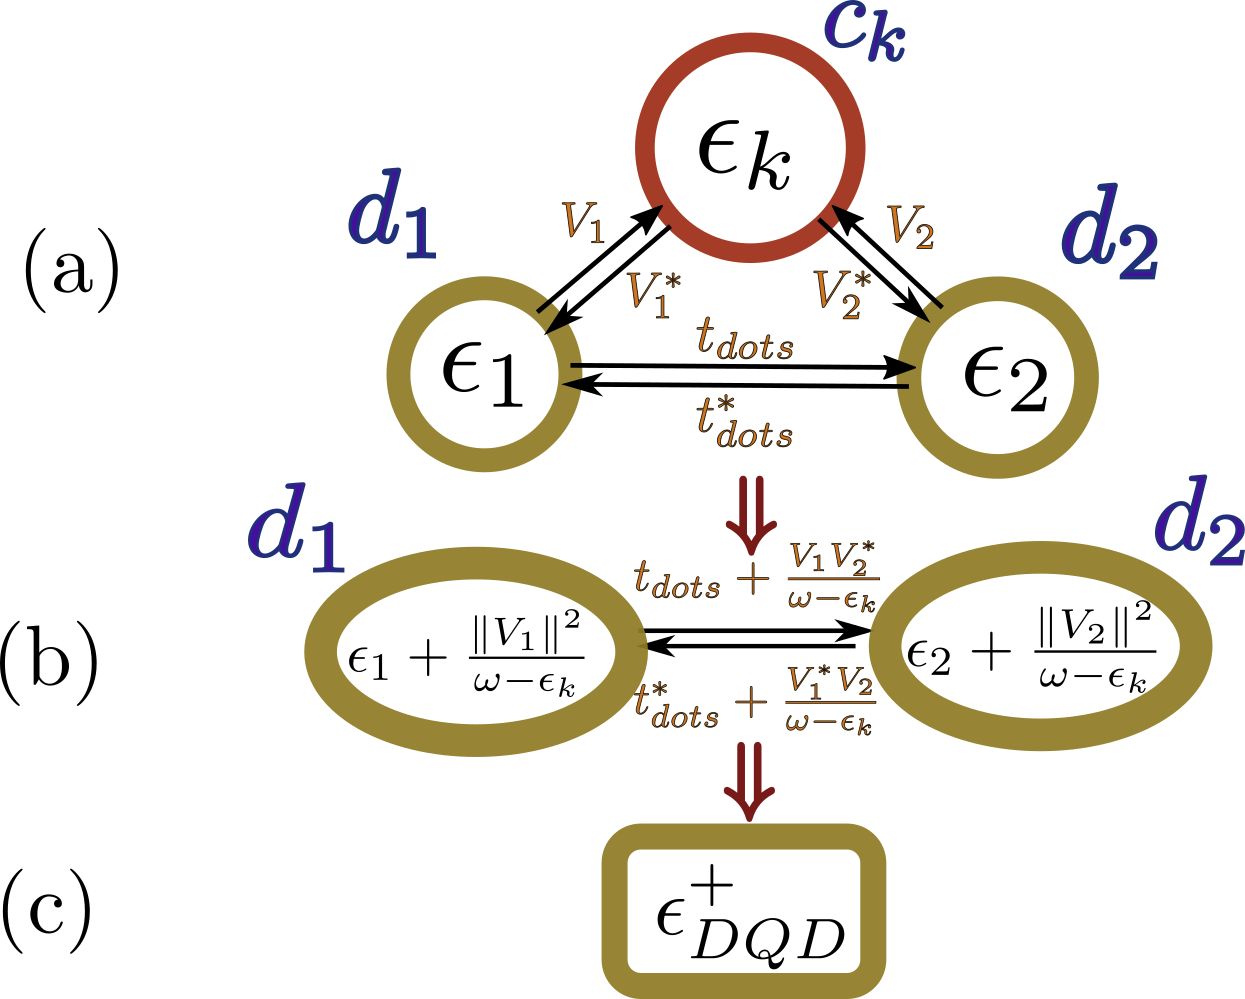
\includegraphics[scale=0.3]{IMAGES/Graphs/DQD-Pro.png}
    \caption{  \label{fig:graphDQD} Graph representation of Gauss-Jordan elimination a) Graph $\GDQD$ b) After the elimination of vertex $c_k$, the energies of dots $d_1$ and $d_2$, and the coupling parameter are changed. c) After Gaussian elimination of dot $2$ the energy of the remaining dot $\epsilon_DQD^+$ represents the transport information through $d_1$ of the entire DQD. \protect\Source{}}
    
\end{figure}


The algorithm consists in the following: Each step of Gauss-Jordan elimination leads to a new graph with different energies and couplings. The elimination of a row and column is equivalent to eliminate the corresponding vertex in the graph. For instance, lets eliminate the first row and column of the matrix in \eqref{eq:MatrixDQD}. For it we just need to subtract the rank-$1$ matrix with the same first row and first column
\begin{align}
       & \left[\begin{array}{ccc}
    \omega-\epsilon_{k} & -V_{2} & -V_{1}\\
    -V_{2}^{*} & \omega-\epsilon_{2} & -t_{dots}\\
    -V_{1}^{*} & -t_{dots}^{*} & \omega-\epsilon_{1}
    \end{array}\right]-\left[\begin{array}{ccc}
    \omega-\epsilon_{k} & -V_{2} & -V_{1}\\
    -V_{2}^{*} & \frac{V_{2}^{*}V_{2}}{\omega-\epsilon_{k}} & \frac{V_{2}^{*}V_{1}}{\omega-\epsilon_{k}}\\
    -V_{1}^{*} & \frac{V_{2}V_{1}^{*}}{\omega-\epsilon_{k}} & \frac{V_{1}^{*}V_{1}}{\omega-\epsilon_{k}}
    \end{array}\right] \\ &= \left[\begin{array}{ccc}
    0 & 0 & 0\\
    0 & \omega-\epsilon_{2}-\frac{V_{2}^{*}V_{2}}{\omega-\epsilon_{k}} & -t_{dots}-\frac{V_{2}^{*}V_{1}}{\omega-\epsilon_{k}}\\
    0 & -t_{dots}^{*}-\frac{V_{2}V_{1}^{*}}{\omega-\epsilon_{k}} & \omega-\epsilon_{1}-\frac{V_{1}^{*}V_{1}}{\omega-\epsilon_{k}}
    \end{array}\right]
    \label{eq:Gauss-Jordan} 
\end{align}

The graph associated to this new matrix can be observed in \ref{fig:graphDQD}(b) where operator $c_k$ has been removed. It is possible to associate the correction to the the energies and couplings to the possible walks passing through the vertex $c_k$.  For instance $d_1$'s energy $\epsilon_1$ receives an extra-term $\frac{V_{1}^{*}V_{1}}{\omega-\epsilon_{k}}$ representing an additional walk  from $d_1$ to $d_1$ passing through  $c_k$. The same logic can be applied to the other coupling terms. The correction to $t_{dots}$ is $\frac{V_{1}^{*}V_{2}}{\omega-\epsilon_{k}}$ which corresponds to a path from $d_1$ to $d_2$ passing through the eliminated vertex $c_k$. Note that this term includes the multiplication of both couplings $V_1, V_2*$ divided by the difference of $\omega$ with the self-energy $\epsilon_k$ of the vertex. This correspondence between the energy correction and eliminated paths through the graph makes the "vertex-elimination" process a straightforward task. 

We now proceed to eliminate vertex $d_2$, which leaves just a single vertex as  shown in \ref{fig:graphDQD}(c). The self-energy of it can be readily computed with the previous path elimination idea which gives 
\begin{equation}
    \epsilon^+_{DQD}=\epsilon_{1}+\sum_{\mathbf{k}}\frac{V_{1}V_{1}^{*}}{\omega-\epsilon_{\mathbf{k}}}+\frac{\left\Vert t_{dots}+\sum_{\mathbf{k}}\frac{V_{1}V_{2}^{*}}{\omega-\epsilon_{\mathbf{k}}}\right\Vert ^{2}}{\omega-\epsilon_{2}-\sum_{\mathbf{k}}\frac{V_{2}V_{2}^{*}}{\omega-\epsilon_{\mathbf{k}}}},  \label{eq:EnDQD}
\end{equation}
\noindent where we selectively included the $\sum_k$-terms in the places where $k$ appeared. 

As a result of  Gauss-Jordan elimination, the linear equation in \eqref{eq:MatrixDQD} has evolved into the trivial form 
\begin{equation}
\left[\begin{array}{ccc}
0 & 0 & 0\\
0 & 0 & 0\\
0 & 0 & \omega-\epsilon_{DQD}^{+}
\end{array}\right]\left[\begin{array}{c}
\Green{c_{\mathbf{k}},d_{1}^{\dagger}}\\
\Green{d_{2},d_{1}^{\dagger}}\\
\Green{d_{1},d_{1}^{\dagger}}
\end{array}\right]=\left[\begin{array}{c}
0\\
0\\
1
\end{array}\right].
\end{equation}
The Green function is then 
\begin{align}
\Green{d_{1},d_{1}^{\dagger}}=\frac{1}{\omega -  \epsilon^+_{DQD}} =\left[\left(\omega-\epsilon_{1}-\sum_{\mathbf{k}}\frac{V_{1}V_{1}^{*}}{\omega-\epsilon_{\mathbf{k}}}\right)-\frac{\left(t_{dots}+\sum_{\mathbf{k}}\frac{V_{1}V_{2}^{*}}{\omega-\epsilon_{\mathbf{k}}}\right)\left(t_{dots}+\sum_{\mathbf{k}}\frac{V_{1}V_{2}^{*}}{\omega-\epsilon_{\mathbf{k}}}\right)^{*}}{\omega-\epsilon_{2}-\sum_{\mathbf{k}}\frac{V_2V_{2}^{*}}{\omega-\epsilon_{\mathbf{k}}}}\right]^{-1}. \label{eq:SumSolGreen} 
\end{align}
\noindent This Green function will appear again in the last chapter when solving the double dot-Majorana system.    
% the inverse of the green function $G_{d_1d^\dagger_1}$. The final result is then 

% \begin{equation}
    % \Green{d_{1},d_{1}^{\dagger}}=\left[\left(\omega-\epsilon_{1}-\frac{V_{1}V_{1}^{*}}{\omega-\epsilon_{\mathbf{k}}}\right)-\frac{\left(t_{dots}+\frac{V_{1}V_{2}^{*}}{\omega-\epsilon_{\mathbf{k}}}\right)\left(t_{dots}+\frac{V_{1}V_{2}^{*}}{\omega-\epsilon_{\mathbf{k}}}\right)^{*}}{\omega-\epsilon_{2}-\frac{\Gamma_{2}^{2}}{\omega-\epsilon_{\mathbf{k}}}}\right]^{-1}. \label{eq:solGreen}
% \end{equation}

% Just one additional correction. Remember that every term including $\epsilon_k$ is summing over all possible energies in the momentum space. We avoided this sum during the process to avoid carrying this term during the process. But it is important to include it know.  

% \begin{equation}
%      \Green{d_{1},d_{1}^{\dagger}}=\left[\left(\omega-\epsilon_{1}-\sum_{\mathbf{k}}\frac{V_{1}V_{1}^{*}}{\omega-\epsilon_{\mathbf{k}}}\right)-\frac{\left(t_{dots}+\sum_{\mathbf{k}}\frac{V_{1}V_{2}^{*}}{\omega-\epsilon_{\mathbf{k}}}\right)\left(t_{dots}+\sum_{\mathbf{k}}\frac{V_{1}V_{2}^{*}}{\omega-\epsilon_{\mathbf{k}}}\right)^{*}}{\omega-\epsilon_{2}-\sum_{\mathbf{k}}\frac{\Gamma_{2}^{2}}{\omega-\epsilon_{\mathbf{k}}}}\right]^{-1}. \label{eq:SumSolGreen}
% \end{equation}

\subsection{Graph Algorithm \label{sec:Algorithm}}

In this part we summarize the steps of the Graph-Gauss-Jordan elimination process to compute the Green function  $\Green{d,d\dagger}$ of an operator $d$:
\begin{enumerate}
    \item Computing the transport equations with the second term of the Green function fixed in the creation operator $d^\dagger$ at all equations. 
     \item  Setting up the  graph associated to the transport system. The self-energy of each vertex is initialized as $\omega$ minus the corresponding diagonal term.  The edge weights are given by the coupling of the off-diagonal terms multiplied by $-1$. 
    \item Eliminating the vertexes of the graph one by one. Each vertex-elimination process carries the following steps.
    \begin{enumerate}
        \item Computing the extra-terms of the energies and couplings based on the walks passing through the eliminated vertex.
        \item Removing this vertex from the graph. 
        \item Iterating till there is only one  vertex.
        \end{enumerate}
    \item The energy in the remaining vertex $d$ is the self- energy $\epsilon_d = \omega -\frac{1}{ \Green{d,d^\dagger}}$ .
\end{enumerate}
This algorithm will be our main method to find the Green function and therefore the density of states of any non-interacting system.  


% However this method lacks of any useful intuition that could help us  to  solve more complex systems. This remarks the  importance of pursuing alternative methods. \\




% Let $v_1$ and $v_2$ be two operators in $\GDQD$. If an operator $v_2$ appears in the right side of the transport equation for vertex $v$, the graph will have  a directed edge from $v_2$ to $v_1$. A weight is assign to this edge given by the coefficient of $v_2$ in $v_1$'s transport equation. Note that this relation is reciprocal since the Hamiltonian is hermitian. Hence if there is an arrow from $v_1$ to $v_2$ with weight $t$, then there there will be an opposite arrow from $v_2$ to $v_1$ with weight $t^*$. e.g. In this case, the tree operators  $d_{1\downarrow},d_{2},c_{\boldsymbol{k}}$ are connected. The weights of these connections are observed in \ref{fig:graphDQD}.\\



% Now, the Green functions $\Green{d_{1},d_{1}^{\dagger}}$ will always have the form $\frac{1}{\omega-E} $ where $E$ is an energy. This form is also observed in \eqref{eq:solGreen}.  Looking at equation \eqref{eq:green1},  observe that if $\Green{d_{2},d_{1}^{\dagger}}$ and $\sum_{\mathbf{k}}\Green{c_{\mathbf{k}},d_{1}^{\dagger}}$ are multiples of $\Green{d_{1},d_{1}^{\dagger}}$ (i.e $\Green{d_{2},d_{1}^{\dagger}}=\eta_{2}\Green{d_{1},d_{1}^{\dagger}},\Green{c_{\mathbf{k}},d_{1}^{\dagger}}=\eta_{\boldsymbol{k}}\Green{d_{1},d_{1}^{\dagger}})$ , the result for $\Green{d_{1},d_{1}^{\dagger}}$ will be 
% \begin{equation}
%     \Green{d_{1},d_{1}^{\dagger}}=\frac{1}{\omega-\epsilon_{1}-\sum_{\boldsymbol{k}}V_{1}^{*}\eta_{\boldsymbol{k}}+t_{dots}\eta_{2}}.
% \end{equation}

% Hence to obtain $\Green{d_{1},d_{1}^{\dagger}}$ we need to find $\eta_{\boldsymbol{k}}$ and $\eta_{2}$. Now note from equation \eqref{eq:green2} that $\left(\omega-\epsilon_{\boldsymbol{k}}\right)\eta_{\boldsymbol{k}}=V_{1}+V_{2}\eta_{2}$

% \begin{equation}
% \Green{d_{1},d_{1}^{\dagger}}=\frac{1}{\omega-\epsilon_{1}-\sum_{\boldsymbol{k}}\frac{V_{1}^{*}V_{1}}{\omega-\epsilon_{\boldsymbol{k}}}+V_{1}^{*}V_{2}t_{dots}\eta_{2}\eta_{2}}    
% \end{equation}


% Now, probably at this point you might already know what is happening here. Basically the energy $E$ represents the sum of all possible transitions in the graph that start and finish at $d_{1}$ . The first term is $\epsilon_{1}$, which is the energy of dot $1$. The next term is $\frac{V_{1}^{*}V_{1}}{\omega-\epsilon_{\boldsymbol{k}}}$ which represents the transition $d_{1}\rightarrow c_{k}\rightarrow d_{1}$. Note that $\frac{V_{1}^{*}V_{1}}{\omega-\epsilon_{\boldsymbol{k}}}$ is basically the energy needed to go from $d_{1}$ to $c_{\boldsymbol{k}}$ and coming back divided by the energy "cost" of passing through $c_{\boldsymbol{k}}$ which is $\omega-\epsilon_{\boldsymbol{k}}$. The sum over $\textbf{k}$ can be ignored in this analysis. Now we can then explain why the last term in \eqref{eq:solGreen} is 
% \begin{equation}
%     \frac{\left(t_{dots}+\sum_{\mathbf{k}}\frac{V_{1}V_{2}^{*}}{\omega-\epsilon_{\mathbf{k}}}\right)\left(t_{dots}^{*}+\sum_{\mathbf{k}}\frac{V_{1}^{*}V_{2}}{\omega-\epsilon_{\mathbf{k}}}\right)}{\omega-\epsilon_{2}-\sum_{\mathbf{k}}\frac{\Gamma_{2}^{2}}{\omega-\epsilon_{\mathbf{k}}}}. \label{term}
% \end{equation}

% Firs note that $\left(t_{dots}+\sum_{\mathbf{k}}\frac{V_{1}V_{2}^{*}}{\omega-\epsilon_{\mathbf{k}}}\right)$ is the energy needed to go from $d_{1}$ to $d_{2}$. This could occur by passing through $c_{\boldsymbol{k}} \ \left(\sum_{\mathbf{k}}\frac{V_{1}V_{2}^{*}}{\omega-\epsilon_{\mathbf{k}}}\right)$ or going directly to $d_ 2$ $\left(t_{dots}\right)$. The term is multiplied by $\left(t_{dots}^{*}+\sum_{\mathbf{k}}\frac{V_{1}^{*}V_{2}}{\omega-\epsilon_{\mathbf{k}}}\right)$ which represents the opposed transition from $d_{2}$ to $d_{1}$.  Finally, we  divide this by the cost of passing through $d_{2}$ and $c_{\boldsymbol{k}}$. This is basically to multiply by the green function taking the point $d_{1}$ out of $\GDQD$ . This green function is


% \begin{equation}
%     \GreenG{d_2,d_2^\dagger}{\GDQD-d1}= \frac{1}{\omega-\epsilon_{2}-\sum_{\mathbf{k}}\frac{\Gamma_{2}^{2}}{\omega-\epsilon_{\mathbf{k}}}}.
% \end{equation}
% where $\GreenG{d_2,d_2^\dagger}{\GDQD-d_1}$ is the green function of $d_2,d_2^\dagger$ in the smaller graph $\GDQD-d_1$. 

% The last equation not only explains the meaning of term \eqref{term} in equation \eqref{eq:solGreen}. It also gives us an iterative method to find the green function. To understand this, note that the solution in \eqref{eq:solGreen} can also be written as 

% \begin{equation}
% \left( \GreenG{d_{1},d_{1}^{\dagger}}{\GDQD} \right) ^{-1}= \omega - \epsilon_1- \sum_\textbf{k} E_{d_1c_k}^{\GDQD-d_2} \GreenG{c_\textbf{k}c^\dagger_\textbf{k}}{\GDQD-d_2-d_1}  - E_{d_1d_2}^{\GDQD} \GreenG{d_2,d_2^\dagger}{\GDQD-d_1} . \label{eq:solGreen2}
% \end{equation}
% Where $E_{d_1c_k}^{\GDQD-d_2} = \sum_{\boldsymbol{k}}\frac{V_{1}^{*}V_{1}}{\omega-\epsilon_{\boldsymbol{k}}} $  represents the accumulated energy of going from $d_1$ to $c_k$ and coming back. The upper-index $\GDQD-d_2$ represents that at this step the second dot is ignored. Similarly $E_{d_1d_2}^{\GDQD}$ is the numerator of \eqref{term}. It represents the energy accumulated in at going from $d_1$ to $d_2$. Since this time no point is ignored, the upper-index remains as $\GDQD$. \\

% Now the amazing thing about the last equation is that it decomposes the green function $\GreenG{d_{1},d_{1}^{\dagger}}{\GDQD}$  into green functions of smaller graphs. This gives an iterative process to compute green functions using induction in graphs .  Now, as you might see, the complexity of these green functions reduce strongly after a single point is removed out of the graph . This makes green function computation a pretty simple task using the graph method. 

% \Jesus{I promise a real proof of this fact to be included in the abstract. The idea is using induction in graphs  \ref{sec:AbsGraphmethod}. }

\subsection{Non-interacting DOS in a  double quantum dot coupled to a lead \label{sec:GreedDQD}}


In this subsection, we describe the remaining steps to obtain the density of states of the double quantum dot from the Green function \eqref{eq:SumSolGreen}. We will plot the results and observe the evolution of the DOS while tuning the parameters of the model. 

First note that equation \eqref{eq:SumSolGreen} depends on the term $\sum_{\boldsymbol{k}}\frac{V_{i}^{*}V_{j}}{\omega-\epsilon_{\boldsymbol{k}}}$, which describes the broadening of the DOS when the QD enters in contact with the lead. This broadening is usually named $\Gamma_i=V_{i}^{*}V_{i}$ (Or $\Delta$ depending on the text book). 
% $$-\Gamma_i = \sum_{\boldsymbol{k}}\frac{V_{1}^{*}V_{1}}{\omega-\epsilon_{\boldsymbol{k}}}. $$
In general, $V_i$  is a function of $\textbf{k}$. However, in the limit of flat-band we can assume that $V_i $ is constant. Therefore, it is enough to integrate
\begin{equation}
    \sum_{\boldsymbol{k}}\frac{1}{\omega-\epsilon_{\boldsymbol{k}}+is}=\int_{-D}^{D}\frac{d\epsilon_{\boldsymbol{k}}}{\omega-\epsilon_{\boldsymbol{k}}+is}=-\ln\left(\frac{D-\epsilon_{\boldsymbol{k}}+is}{-D-\epsilon_{\boldsymbol{k}}+is}\right)\xrightarrow[D\rightarrow\infty]{}-i , 
\end{equation}
\noindent where we assumed that there is a maximum  energy cutoff $D$ going to infinity in the wide-band limit. Hence 
\begin{equation}
   -i\Gamma_i = \sum_{\boldsymbol{k}}\frac{V_{i}^{*}V_{i}}{\omega-\epsilon_{\boldsymbol{k}}}.
\end{equation}



We can replace this in equation \eqref{eq:SumSolGreen} to obtain the real expression for the green function $\Green{d_1,d_1^\dagger}$. The terms of the form $V_1V_2^*$ can be replaced for $\sqrt{\Gamma_1\Gamma_2}$, supposing there is no additional complex phase.

Now, remember from \eqref{eq:Density of States} that the DOS $\rho$ depends on the imaginary factor of the Green Function $\Green{d_1,d_1^\dagger}$. This term depends in the broadening $\Gamma$. If $\Gamma = 0$ the density of states will be $0$ as well. At any other case, one of the dots should be attached to the lead. Let $\Gamma_1$ be the broadening of this dot. We will take $\Gamma_1$ as our  unit for the rest of this thesis.  

In \ref{fig:GreenDQD} we can observe the evolution of the Density of States under certain processes. Each plot includes an inset showing the model applied to the figure. The coupling in purple indicates the tuning variable. We set $e_1 = e_2 = 0$ so that both dots satisfy PHS. The primary results are the 

   % ----------------SUPER FIGURE ---------------------------
    \begin{figure}[t]
        \centering
         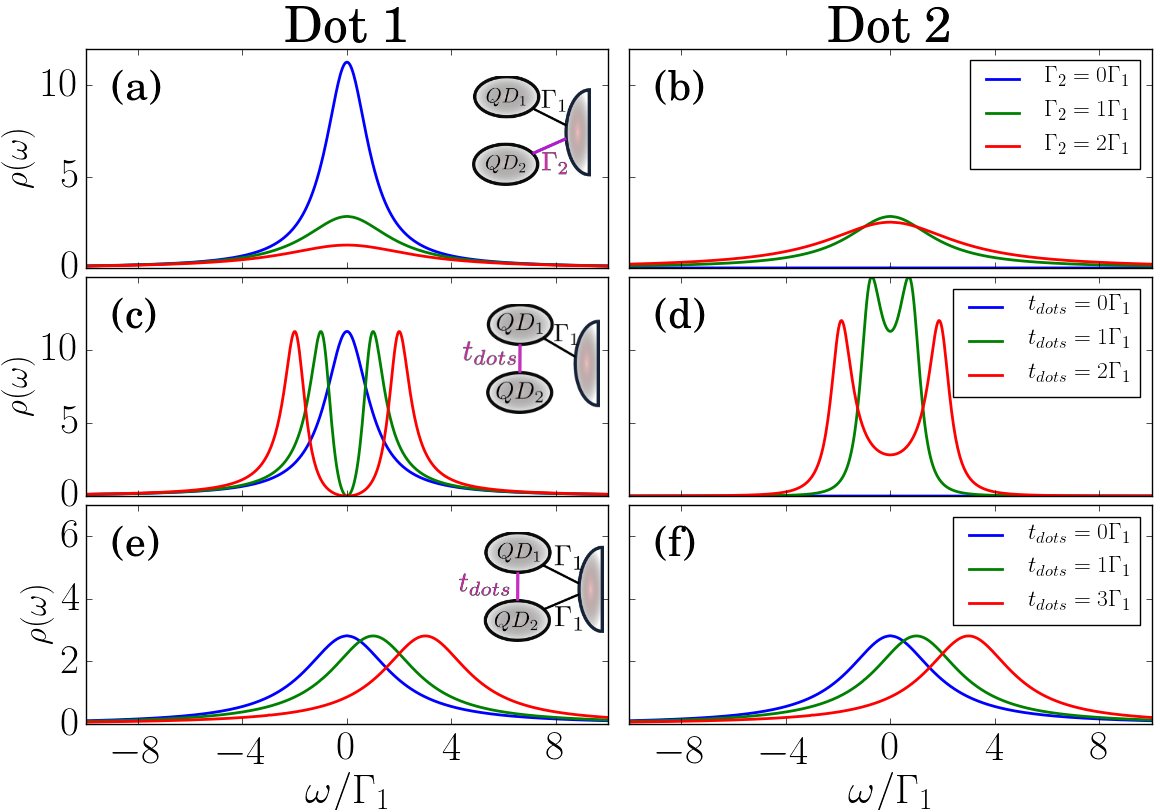
\includegraphics[scale=0.47]{IMAGES/DQD/Non-interacting.png}
         \caption{\label{fig:GreenDQD} Evolution of the density of states at each QD (Left: dot 1, Right: dot 2) at three distinct arrangements of DQD-lead coupling. The inset at the first column depicts the type of coupling. The purple line represents the tuning variable. The energy unit is $\Gamma_1$. $e_1 =e_2 =0$ in all arrangements. (a),(b) The lead is connected to both QDs. Tuning variable: $\Gamma_2$. (c)(d) Indirect coupling of the second dot through dot one. Tuning variable: $t_{dots}$. (e)(f) Triangular coupling. Tuning variable: $t_{dots}$.  
         \protect\Source{   }}
    \end{figure}
% ----------------SUPER FIGURE ---------------------------


\begin{enumerate}
    \item \textbf{Coupling QD2. \ref{fig:GreenDQD}(a)(b):}  At $\Gamma_2=0$  the second dot is decoupled, hence the first dot's DOS is the same of a single dot case. The maximum height is achieved at  $\rho \pi \Gamma_1 =1$ and the width of this peak is approximately  $\Gamma_1$, just as in Figure \ref{fig:specDots}. When the second dot is attached $\Gamma_2 >0$, the density of states is divided between both dots. At $\Gamma_1 = \Gamma_2$ the DOS at the Fermi energy is equal to $\frac{1}{4\pi\Gamma}$ for both dots. For higher values of $\Gamma_2$, the DOS in the second dot is higher than in the first one.  
    
 

    \item \textbf{Indirect Coupling of QD2. \ref{fig:GreenDQD}(c)(d):} This case is interesting. When the second dot is connected indirectly through the first dot, quantum inference splits the central peak in two new states. We will observe later that in the interacting case this procedure can also destroy the Kondo signature. Note that the higher the coupling $t_{dots}$ is, the greater is the gap between the states. We will usually take $t_{dots} = 2\Gamma_1$ to make these gap more visible in the NRG simulations. 
    % This has interesting consequences when combined with Majorana physics.
    \item \textbf{Breaking Particle Hole Symmetry. \ref{fig:GreenDQD}(e)(f):}
    Suppose we have $\Gamma_2 = \Gamma_1$. The "triangular connections" break Particle Hole Symmetry, with the central peak detuning to the positive part of the spectrum. We will avoid this situation during this project, because because PHS-breaking  will prevent the Majorana to tunnel inside the DQD. Hence, this model won't lead to any interesting result on Majorana manipulation. 
\end{enumerate}



% \begin{figure}[H]
%      \centering
    
%      \subfloat[Attaching QD2 to the lead \label{fig:DQD-G2}]{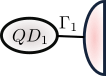
\includegraphics[scale=0.6]{IMAGES/DQD/g1g2-m.png}} \\
%     \subfloat[Indirect connection of QD2 \label{fig:DQD-tdots}]{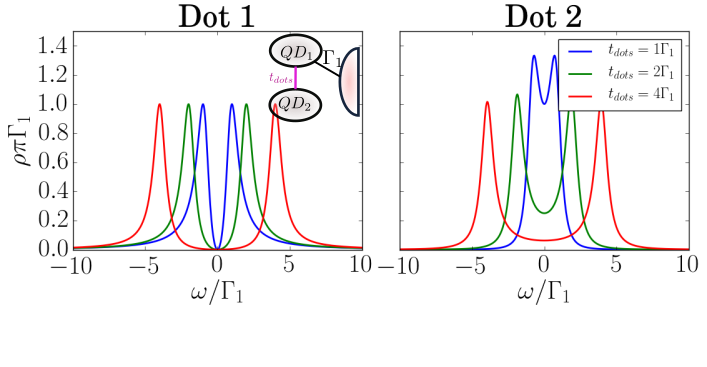
\includegraphics[scale=0.6]{IMAGES/DQD/tdots-m.png}}\\
%     \subfloat[Breaking PHS with triangular connection \label{fig:DQD-PHS}]{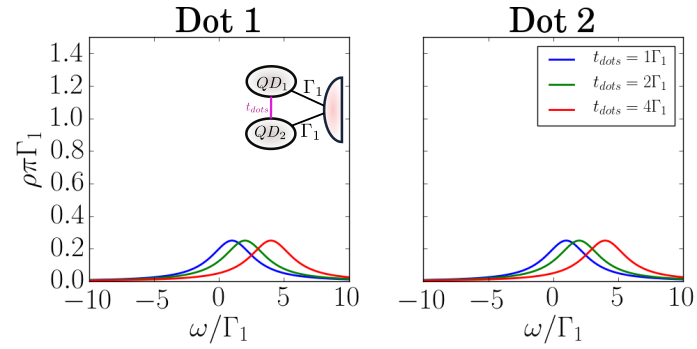
\includegraphics[scale=0.6]{IMAGES/DQD/phs-m.png}}
%      \caption{\label{fig:GreenDQD} For the tree cases we considered $e_1 =e_2 =0$. The inset shows the set-up. At each case the purple coupling shows the tuning variable. \protect\Source{   }}
% \end{figure}














% ------------------------------------------NRG----------------------
% ---------NRG-------------------------------------------------------
% ------------------ NRG --------------------------------------------
% -----------------------------------------------------NRG------------



\section{The Numerical Renormalization Group\label{sec:The-Numerical-Renormaliztion} (NRG) }

The numerical renormalization group is renown for providing the most successful and complete explanation of the Kondo problem. of integrating the strong correlations in coulomb interacting systems. In this chapter, we will review the main ideas of the NRG algorithm including the logarithmic discretization, the construction of Wilson's chain and the iterative diagonalization in symmetry blocks. At the end, we will give some specifications about our code and we will show its results in the model of a double quantum dot attached to a metallic lead. 

\subsection{From the Renormalization Group to  Wilson's Chain \label{subsec:Logarithmic}}

%-------------------------------------------------------
\begin{figure}[hbt]
\centering
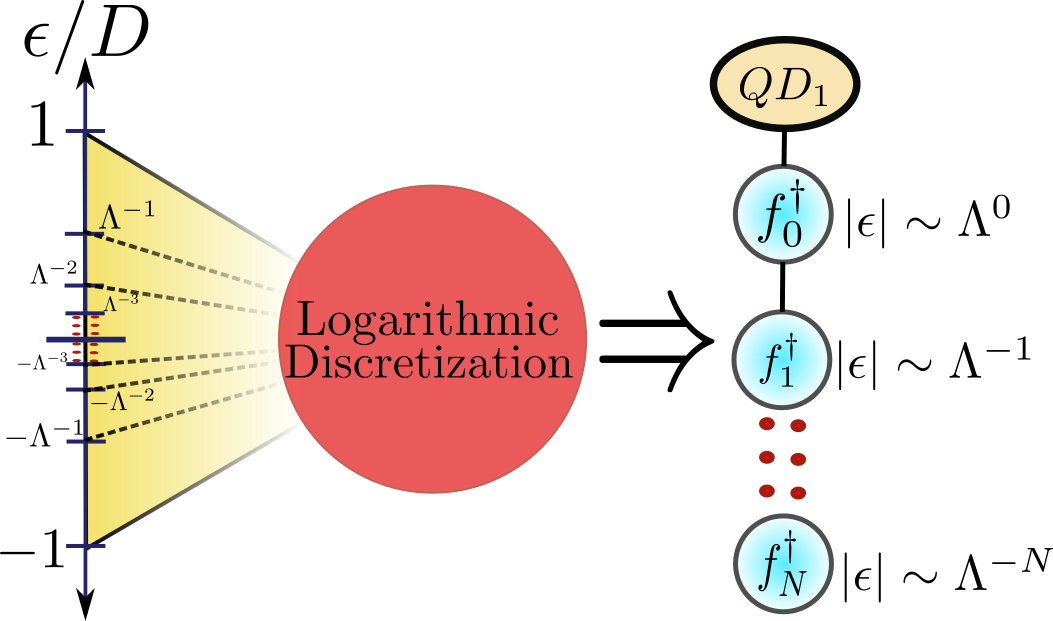
\includegraphics[scale=0.45]{IMAGES/DQD/NRG-Final.png}\caption{\label{fig:Discretization}
NRG algorithm: The logarithmic discretization of the conduction band according to the discretization parameter $\Lambda$. The system with the lead attached to the QD-impurity is mapped to the Wilson's chain, such that each step of the chain contains the contributions at different energy scales $\Lambda^{-N/2}$. \protect\Source{   } }
\end{figure}
%--------------------------------------------------

 The real meaning of the divergent logarithmic term in the resistivity predicted by Kondo is that important contributions at low-energy scales caused by the strong quantum correlations in the system are being neglected by perturbation theory. This problem can be solved by introducing ideas from renormalization group theory. A renormalization approach is more adequate for this type of problem since it assigns an appropriate effective Hamiltonian to each scale of temperature. This provides a more accurate representation of the increasing density of correlated states appearing close the Fermi energy. 

In renormalization group theory, the Hamiltonian transformations are performed by an operator $\mathcal{T}$ that represents an endomorphism in the space of operators. $\mathcal{T}$ generates the semigroup  $\{ 1, \mathcal{T} , \mathcal{T}^2 , \ldots \}$, that defines a complete set of transformations   % transformation of the form
$$ \mathcal{T}[H_0] = H_1, \  \mathcal{T}[H_1] = H_2, \ldots , \mathcal{T}[H_N] = H_{N+1} , \ldots$$
\noindent If $\mathcal{T}$ is a contracting map  \footnote{ Let $\mathcal{O}$ be a set of operators, then $T$ is a contracting map if $\mathcal{T}[\mathcal{O'} ] \subset \mathcal{O'}$ for every $\mathcal{O'} \subset \mathcal{O}$ .} then it is known that this set of operations should eventually lead to a fix point $ \mathcal{T}^N[H] \xrightarrow{N\rightarrow\infty} H^*$ such that $\mathcal{T}[H^*] = H^*$. In numerical simulations, $N $ will only increase up to a value where $H_N$ is close enough to the fix point $H*$ so that no new significant contributions to the Hamiltonian are obtained. For the purposes of this project, taking $N = 51$ will be enough  for the NRG code to converge. 

%Maybe the most important characteristic of the Kondo effect is that leading contributions to the conductivity are caused by strong correlations with the conduction band appearing at low energy scales. This is the reason of the divergent logarithmic term in the Kondo resistivity. 

In the 1970's G.Wilson used this theory to create the famous Numerical Renormalization Group (NRG) \citep{bulla_numerical_2008,wilson_renormalization_1975,krishna-murthy_renormalization-group_1980}. His main idea was to perform a logarithmic discretization of the conduction band in the lead as shown in \ref{fig:Discretization}.(Left).  Taking into account that the leading contributions to the conductance occur at states close to the Fermi energy $\omega = 0$, we can define a cut-off $( \vert \omega \vert < D)$ so that the rest at higher contributions are not relevant.Then we use D to rescale the energy interval. As you can observe in the figure, the QD is coupled to all these energy states at the same time. The logarithmic discretization gives more relevance to the low energy scales by assigning a different Hamiltonian coupling to each one of them.  The discretized intervals are determined by a variable $\Lambda>1$. This value has certain relevance on the convergence of the code. If it is selected to small $(\Lambda \sim 1)$ it might never converge, but if it is too high it could produce misleading results. In this thesis we use a definite value of $\Lambda = 2.5$. This value was tested several times, giving positive results. 

To complete this idea, the NRG code maps the Hamiltonian of the QD-lead system to the Wilson's chain shown in \ref{fig:Discretization}(Right), so that each step of the chain contains the contributions of a different energy scale. A detailed description of this map is included in the Appendix \ref{sec:LogarithmicDisc}.After these steps we obtain a chain Hamiltonian of the form 

\begin{equation}
H=H_{d}+D\sum_{\sigma}\Biggl[\sqrt{\frac{2\Gamma}{\pi D}}\left(d_{\sigma}^{\dagger}f_{0\sigma}+f_{0\sigma}^{\dagger}d_{\sigma}\right)+\frac{1}{2}\left(1+\Lambda^{-1}\right)\sum_{n=0}^{\infty}\Lambda^{\frac{-n}{2}}\xi_{n}\left(f_{n\sigma}^{\dagger}f_{n+1,\sigma}+f_{n+1\sigma}^{\dagger}f_{n\sigma}\right)\Biggr].\label{eq:Newchain-Hamiltonian}
\end{equation}


\noindent In the flat-band approximation the parameters $\xi_{n}$ can be obtained analytically \citep{bulla_numerical_2008}
\[
\xi_{n}=\frac{1-\Lambda^{-n-1}}{\left(1-\Lambda^{-2n-1}\right)^{\frac{1}{2}}\left(1-\Lambda^{-2n-3}\right)^{\frac{1}{2}}}.
\]


%The formal recursive-solution of this problem can be found in \citep{bulla_numerical_2008}. 
From equation \eqref{eq:Newchain-Hamiltonian}  we define the following sequence of shell Hamiltonians

\begin{equation}
H_{N+1}=T\left[H_{N}\right]=\Lambda^{\frac{1}{2}}H_{N}+\xi_{N}\left(f_{N+1,\sigma}^{\dagger}f_{N,\sigma}+f_{N,\sigma}^{\dagger}f_{N+1,\sigma}\right), \label{eq:NRG-Renormalization}
\end{equation}

\noindent with 
\begin{equation}
H_{-1} := \frac{2 H_d\Lambda^{-1/2}}{D(1+\Lambda^{-1})}\ ,\ \xi_{-1}=\sqrt{\frac{2\Gamma}{\pi D}}.\label{eq:H-1}
\end{equation}

Note that at each step  $H_N$ is being rescaled by a factor $\Lambda^{1/2}$ before including the following contribution.  This is performed iteratively to eliminate the high order excitations, which allows to obtain an effective model valid for the lower energies. In consequence, each Hamiltonian $H_N$ represents only the physics that is relevant at the energy scale $\Lambda^{-N/2}$. 

%Then the initial Anderson model can be recovered in the limit 
%\begin{equation}    
%H = \lim_{N \rightarrow \infty } \frac{1+\Lambda^{-1}}{2}\Lambda^\frac{ N-1 }{2} H_N
%\end{equation}
On the other hand, the Renormalization Group transformation $\mathcal{T}$ can be defined as 

$$\mathcal{T}^N H_{-1} =  \frac{1+\Lambda^{-1}}{2}\Lambda^\frac{ -N }{2} H_N$$

\noindent In the limit $\xrightarrow{N\rightarrow\infty}$ we should recover the initial Anderson Hamiltonian. In addition, note that the leading coefficients of the contributions to each Hamiltonian $H_N$ are given by 
\[
\Lambda^{\frac{-N}{2}}\xi_{N}\xrightarrow{N\rightarrow\infty}\frac{\Lambda^{\frac{-N}{2}}\left(1-\Lambda^{-N}\right)}{1-\Lambda^{-2N}}\sim\frac{\Lambda^{\frac{-N}{2}}}{1+\Lambda^{-N}},
\]
\noindent which decays exponentially with the length of the chain. Therefore, we may thing that at some point these new contributions will be so small that the that the map $\mathcal{T}$ will eventually converge. Formally the theory for NRG convergence is too complex for this thesis. However the results show that the operator that truly converges is $\mathcal{T}^2$ and not $\mathcal{T}$\cite{krishna-murthy_renormalization-group_1980}. This has important consequences, for instance the convergence of the code has to be analyzed on odd and even values of $N$ separately. 

To this point, the equation \eqref{eq:Newchain-Hamiltonian} and the derived limit of $H_N$ to the Anderson Hamiltonian are exact expressions. The first approximations will be performed in the following section which descries the iterative diagonalization of the shell Hamiltonians.
 
 \subsection{Iterative Diagonalization \label{subsec:IterativeDiag}}

\begin{figure}[bt]
\centering
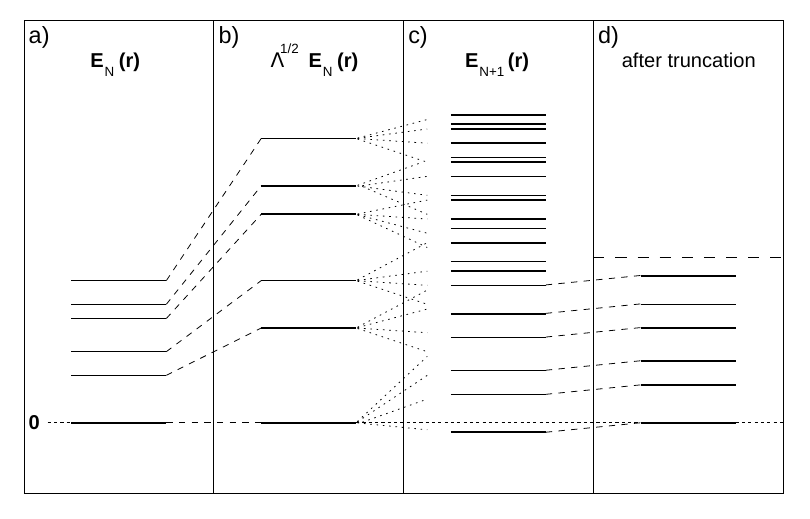
\includegraphics[scale=0.5]{IMAGES/DQD/cutting.png}
\caption{ \label{fig:IterativeDiagonalization} Schematic representation of the spectrum in the iterative diagonalization process. a)$\rightarrow$b): Rescaling. b)$\rightarrow$c): Including next site and diagonalizing. c)$\rightarrow$d): Truncation of high energy states . \protect\Source{ Adapted from \cite{bulla_numerical_2008} } }
\end{figure}


 The diagonalization begins with the dot-impurity Hamiltonian $H_{-1}$, which must be written in matrix form according to a defined basis. The other steps can be defined by induction.  Suppose that the spectrum of $H_{N}$ is diagonal on a given basis. Then the NRG code performs each of the following steps:

\begin{enumerate}
 	\item Rescaling the spectrum of $H_{N}$ by $\Lambda^{\frac{1}{2}}$ as defined in \eqref{eq:chain-Hamiltonian}. \ref{fig:IterativeDiagonalization} (a)$\rightarrow$(b).
 	\item Adding the next step of the chain to form $H_{N+1}$ and diagonalizing the new Hamiltonian such that $H_{N+1} = U_{N+1}^\dagger D_{N+1} U_{N+1}$ . After this step, each of the eigenstates of $H_{N}$ will spit in up to $4$ new energy states (probably degenerate) determined by the new coupling with the  $N+1$ site basis ${\vert 0 \rangle, \vert \up \rangle, \vert \dw \rangle, \vert \up \dw \rangle}$.  \ref{fig:IterativeDiagonalization} (b)$\rightarrow$(c).
 	\item Shifting the spectrum by a certain dephase factor such that the zero of energy is always the ground state.  \ref{fig:IterativeDiagonalization} (c)$\rightarrow$(d).
 	\item Numerical cutting: If the number of states in the system exceeds a definite number (1000 in this thesis) the exceeding higher energy states are neglected \footnote{ This step must be performed carefully to preserve the symmetries of the system. If two states are entangled and one of them is eliminated and the other is not, the program could lead to misleading results. Further discussions to solve this problem are presented in the symmetry subsection.  }. This is in agreement with the previously exposed  idea of eliminating high order excitations to obtain a valid effective model at low energies. \ref{fig:IterativeDiagonalization} (c)$\rightarrow$(d).
 	\item Rotating operators $f_{N,\sigma}$  by $ U_N f_{N,\sigma} U_N^\dagger$ to start the next operation.
\end{enumerate}

The final outcome of this operations will be the complete spectrum of the Anderson model at each energy level. However we still need to talk about an important speed-up to the code obtain when considering the symmetries of the system. 

\subsection{Symmetries \label{subsec:Syms}}

The symmetries of the initial Hamiltonian take a very important role in this iterative diagonalization. Lets suppose that the initial Hamiltonian $H_d$ has certain symmetries classified by the quantum number $S$ . Then $H_d$ can be written  in block Hamiltonians over a basis of the form $\vert S, i\rangle$. A diagnolization process of an square matrix with $L$ rows usually has square order, proportionate to the number of entries $\mathcal{O}\sim L^2$. However, if the matrix is organized in blocks of length $L_j$  such that $\sum_j L_j = L$, then the order of diagonalization will be around $\sum_j L_j^2  $ which is in general much smaller than $(\sum_j L_j)^2 L^2$. Therefore the block diagonalization provides an important numerical speed-up to the algorithm. 

To maintain  this advantage, we must preserve this symmetry structure for the rest of the NRG code. For it, we first need to verify that the picked symmetry also commutes with the hopping terms in the chain Hamiltonian. If so, for each step  $N$ of the NRG algorithm  the $H_N$ Hamiltonian can be written in a block diagonal form with basis 
$\vert S_N, i_N\rangle$. Then it is necessary to define transition rules from the quantum numbers $S_N$ to $S_{N+1}$. By doing this, we assure that the block architecture is transmitted through the entire algorithm, hence reducing the computational time significantly at each step of the NRG chain. This is a key procedure to optimize the algorithm


In the following subsection we will give a example of this symmetry propagation in the model a quantum dot attached to a metallic lead. 




% This block structure simplifies the diagonalization process since the algorithm can diagonalize each block one by one.  This is numerically favorable since the diagonalization of a quadratic matrix  

% takes a quadratic order $n^2$ in a fully entry matrix. Keeping the blocks during the entire NRG 

% Since a numerical diagonalization algorithm have quadratic order $n^2$, it is numerically favorable

%In \ref{sec:Kondo} we observed that the Kondo resistivity had a logarithmic contribution which led to a huge trouble when describing energies bellow the Kondo temperature. This logarithmic term has a  especial meaning which is that the lower energy scales are also relevant. Thus, to solve the Kondo problem it was necessary to create a theory that could efficiently integrate the contributions from all energy scales. In the 1970's G.Wilson created a numerical method that mixed ideas from scalability and renormalization group. This method proofed to be the most efficient form to understand the Kondo effect as well as other impurity problems described by the Anderson Model. 

%Wilson's idea was to discretize the conductance band logarithmically in energy in 
 
%In the 1970's G.Wilson created a numerical method to solve the Anderson model . This method receives the name of Numerical Renormalization Group (NRG) \citep{bulla_numerical_2008,wilson_renormalization_1975,krishna-murthy_renormalization-group_1980}.



% It consists of three basic steps :
% \begin{enumerate}
% \item To perform a numerical discretization of the energy spectrum in logarithmic intervals. 
% \item To map the discretized model onto a semi-infinity chain Hamiltonian. 
% \item  To diagonalize iteratively the chain hamiltonian . 
% \end{enumerate}

% The final result will be the spectrum of the Hamiltonian. Other important properties of the material such as density of states, conductivity, specific heat, susceptibility can also be computed. On this project we are mainly interested in the Density of
% \chapter{The Pursuit of Majorana Fermions \label{chap:Majorana}}



The  Majorana Fermions, so called in the name of the Italian physicist Ettore Majorana, were first defined in the attempt to find a real solution of the Dirac equation. The real field that solves this equation describes a fermion which is its own antiparticle, thus it has no electric charge  nor mass.  Till these days, no fundamental particle with these characteristics has been observed. However, the last decade has been full of excitement as new Majorana quasiparticles have been observed at the edges of topological superconductors.


These topological materials experience phase transitions without passing through a symmetry breaking, hence they cannot be characterized by Landau theory. Instead, these phases of matter are described by  a new type of order determined by the topology of the Brilloin zone. In mathematics, topology is used to describe non-local features of surfaces (or manifolds) that are preserved under smooth deformations. The clich\'e joke of a single-hole cup of coffee that can be softly deformed to a donuts is the preferred picture to explain this concept.
The great insight of topology to condensed matter is that those materials that are attributed a topological characterization are endowed with topological  stability under smooth deformations (or adiabatic evolutions in physicist's language) . The most famous example of this behavior is the integer quantum hall effect whose robust conductivity platoes representing different topological phases allowed to define a resistivity standard, hence having major impact in science and technology.
% have  groundbreaking in the design of high precision devices.

More recently, a new type promising topological material have captivated many physicsts. This is the Majorana wire, inspired in a famous Kitaev's toy model representing a spinless p-wave superconducting chain. Under certain conditions, the Majorana wires experience topological phase transition characterized by the emergence of bizarre zero-modes localized at edges of the wire. Kitaev associated these modes with Majorana quasi-particles  appearing at the boundary of the topological superconducting wires. Then, he pointed out that the combined properties of robustness from topological materials and Majorana's non-abelian statistics could lead to the creation of fault tolerant quantum gates. This fact opened the doors to the search of Majorana fermions in condensed matter physics. 

In this chapter we will present a review of the main topics about Majorana fermions. In the first section \ref{sec:KitaevChain}, we will describe the the Kitaev's chain and the emergence of Majorana zero modes. Next, we will discuss about the real implementations of Majorana chains and the experimental proposals that have been carried on . Finally, we will take a look to new innovations product of coupling QDs with Majorana chains. 



% ------------------------Section: Kitaev *------------------
\section{The Kitaev Chain \label{sec:KitaevChain}}
Kitaev's tight binding toy model  represents a  finite $p$-wave superconducting wire with the following Hamiltonian

\begin{equation}
H = \sum_{i=1}^N \left[ -t(a_i^{\dagger} a_{i+1} + a_{i+1}^{\dagger}a_i) -\mu a_i^{\dagger} a_{i} +  \Delta a_{i}a_{i+1} + \Delta^* a_{i+1}^{\dagger}a_i^{\dagger} \right].  \label{eq:kitaevHam}
\end{equation}

Where $\mu$ is the chemical potential, so that $\mu a_i^{\dagger} a_{i}$ is the energy associated to each step in the chain. $t(a_i^{\dagger} a_{i+1} + a_{i+1}^{\dagger}a_i)$ represents the interaction between neighbouring sites which is determined by the hopping term $t$. The remaining terms describe the superconducting properties of the system as is is established by the BCS theory of superconductivity. $\Delta$ is a complex superconducting parameter with the form  $\Delta = e^{i\theta} \super$. The associated terms represent the Cooper pairs which can be created or annihilated at neighbouring sites of the system.

The form of hamiltonian \prettyref{eq:kitaevHam} favors the possibility of introducing new operators $\gammaA{j}$ and $\gammaB{j}$ such that

\begin{equation}
\gammaA{j} = e^{i\theta /2}a_j+ e^{-i\theta/2 } \ann_j \ \ , \ \ \gammaB{j} = -i(e^{i\theta /2}a_j - e^{-i\theta/2} \ann_j).
\label{eq:MajoranaTrans}
\end{equation}
It is simple check that these operators are self-adjoint $(\gammaA{j}^\dagger = \gammaA{j}, \gammaA{j}^\dagger = \gammaB{j})$. This is a required constraint for the Majorana particles. In addition they satisfy the fermionic anti-commutation relations
\begin{equation}
\begin{aligned}
\{\gammaA{i}, \gammaA{j}\} = \{ & \gammaB{i} , \gammaB{j}\} = 2\delta_{ij}  ,\\ 
  \{\gammaA{i}, \gammaB{j} & \} =0.
\end{aligned} 
\label{MajoranaRel}
\end{equation} 
This allows us to understand the operators $\gammaA{i} , \gammaB{i}$ as Majorana fermions. If we also take the inverse of \prettyref{eq:MajoranaTrans} we obtain that each  (Dirac) fermion in Hamiltonian \eqref{eq:kitaevHam} is composed by two Majorana fermions such that 
$$a_j = \frac{e^{-i\theta/2}}{2}(\gammaA{j}+ i\gammaB{j})$$
We could even adventure to say that these Majorana operators are actually dividing the Dirac fermions into real($\gammaA{}$) and imaginary $(\gammaB{})$ part ,the same way as complex numbers are a composite of two real numbers. 

The new Kitaev Hamiltonian in the Majorana representation looks like 

\begin{equation}
H = \frac{i}{2} \sum_{j=1}^N \left[ -\mu \gammaA{j}\gammaB{j}  + (t- \super) \gammaB{j}\gammaA{j+1} + (t+ \super) \gammaA{j}\gammaB{j+1} \right]+Const,\label{eq:HamMajorana}
\end{equation}

Depending on the values of parameters $\mu, t$ and $\super$ we can identify two regimes represented by the following situations:


%\begin{figure}[t]
%$$\includegraphics[scale=0.5]{KitaevtopPhases.jpg}
%\centering
%\label{top.phases kitaev}
%\caption{{\small \textit{Taken from \cite{bernevig2015topological}. Ilustration of the Kitaev chain for open boundary conditions in the Majorana representation. a)Represents the trivial case where the hopping and the superconducting term approaches to $0$. b) The non-trivial topological phase. The coupling is produced between Majoranas in different Dirac fermions }}}
%\end{figure}

\begin{figure}[hbt]
    \centering
    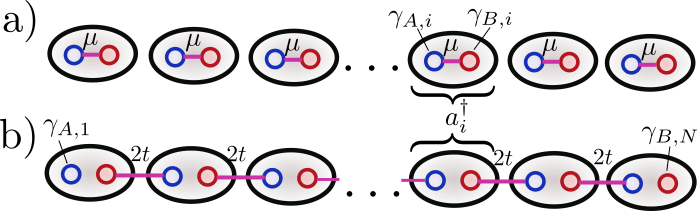
\includegraphics[scale=0.5]{IMAGES/Majorana/KitaevChain.png}
    \label{fig:top.phases kitaev}
    \caption{Illustration of the Kitaev chain for open boundary conditions in the Majorana representation. a)Represents the trivial case where the hopping and the superconducting term approaches to $0$. b) The non-trivial topological phase. The coupling is produced between Majoranas in different Dirac fermions \protect\Source{By the author} }
\end{figure}


\begin{enumerate}
\item{If $\super = t = 0, \mu <0$} Hamiltonian \eqref{eq:HamMajorana} becomes $\frac{-i\mu}{2} \sum_{j} \gammaA{j}\gammaB{j}$ which represents the coupling of the Majoranas in the same Dirac fermion. (See Figure \ref{fig:top.phases kitaev} (a))

\item{If $\super = t > 0, \mu =0$} the situation is much more interesting. The Hamiltonian \eqref{eq:HamMajorana} takes the form $H = 2ti\sum_{j} \gammaA{j}\gammaB{j+1}$. This implies that the coupling is performed between  Majoranas of different Dirac fermions leaving the edge Majorana operators ($\gammaA{1}$ and $\gammaB{N}$) uncoupled (See Figure \ref{fig:top.phases kitaev}b)). Note that these uncoupled Majorana fermions can be at any state without any  repercussion in the energy of the system. This explains the emergence of a  ground state localized at edges of the chain. 
\end{enumerate}

These two situations are representatives of two different phases. The trivial phase occurs for $\frac{\mu}{2t}>1$ and the non-trivial phase appears when $\frac{\mu}{2t}<1$ (See figure \ref{fig:KitaevSpec}). The mean characteristic of the non-trivial phase is the creation of an stable zero-mode. This zero-mode is generated by the  uncoupled Majorana fermions at the edges of the Kitaev chain.  \\



\begin{figure}[t]
    \centering
    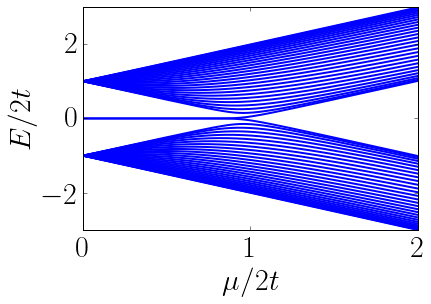
\includegraphics[scale=0.5]{IMAGES/Majorana/Spectrum.png}
    \label{fig:KitaevSpec}
    \caption{Spectrum of Hamiltonian \eqref{eq:HamMajorana} with $30$ sites and $t=\super$ s. Method: Numerical diagonalization. \protect \Source{By the author} }
\end{figure}



% ---------------Subsection: Topological phase transition-------------
\subsection{Topological phase transition}

The two regimes described previously  can be characterized with a topological parameter.  One of the methods for this is following the idea used by \citeauthor{alicea_new_2012}\cite{alicea_new_2012}. The first part is to suppose that we have an infinite chain $(N=\infty)$ in Hamiltonian \eqref{eq:HamMajorana}. The new system is translation invariant, hence we can make a transformation to the momentum space. Then we may rewrite Hamiltonian \eqref{eq:HamMajorana}  as

\begin{equation}
    H = 
    \sum_{k \in BZ} 
    \begin{pmatrix} 
      b_k'  & c_{k}'\\  
    \end{pmatrix}
    H_k 
    \begin{pmatrix} 
      b_{-k}'     \\ 
      c_{-k}' 
    \end{pmatrix}.
    \label{PBCHam2}
\end{equation}

with the Bloch Hamiltonian 

\begin{equation}
H_k = \begin{pmatrix} 
      0    &  \frac{-i \mu}{2} + it \cos k + \super  \sin k  \\ 
       \frac{i \mu}{2} - it \cos k + \super \sin k  &  0 
    \end{pmatrix}
    = (\super \sin k) \sigma_x + (\frac{\mu}{2}- t \cos k) \sigma_y.
\label{sigma}
\end{equation}




\noindent where $\sigma_x$ , $\sigma_y$ are the corresponding Pauli matrices. The Brilloin zone ($BZ$) is the periodic space  $[-\pi , \pi]$ which can be mapped to the unitary circle.   Equation \eqref{sigma} determines  the coordinates of the Bloch Hamiltonian in the base $\{\sigma_x, \sigma_y\}$. We can map these coordinates to the unitary circle by taking the norm of this vector giving
\begin{equation}
     \hat{H}_k= \frac{1}{\sqrt{\super^2 \sin^2 k + (\frac{\mu}{2}- t \cos k)^2}}
     \begin{pmatrix} 
      \super \sin k    \\ 
      \frac{\mu}{2}- t \cos k 
    \end{pmatrix}. 
\end{equation}

Note that $\super^2 \sin^2 k + (\frac{\mu}{2}- t \cos k)^2 \neq 0$ for all the values of $k$ as long as $\frac{\mu}{2t} \neq 1$ . When $\frac{\mu}{2t} = 1$ the $H_{k=0}=0$, so it cannot be normalized. \textbf{This is the same point were the phase transition occurs!}. At any other value of $\frac{\mu}{2t}$ it is possible to normalize $H_{k}$ for all values of $k\in BZ$. The result of mapping $\hat{H}_k$ for all $k$ is a path around the unitary circle. \\

This path can take two forms as we can observe in Figure \ref{fig:topological}. If $\frac{\mu}{2t} > 1$ the path reduced to a line in the upward part of the circle. In the non-trivial phase $\frac{\mu}{2t} < 1$ the path completes the round to the entire circle. Note that this method states a topological difference between the two phases. While the path described by the trivial phase can be contracted to a single dot, the path described by the non-trivial one is a circle that cannot be contracted. \\

Note that to determine whether path of a given phase is of type a) or type b) we only need to check if $\hat{H}_{k=0}$ and $\hat{H}_{k=\pi}$ are the same point or opposite points. This transforms into a simple equation 
\begin{equation}
    \hat{H}_{k=0,y}\hat{H}_{k=\pi,y}=\begin{cases}
1 & \mbox{trivial phase}\\
-1 & \mbox{non-trivial phase}
\end{cases}
\end{equation}
where $\hat{H}_{k=0,y}$ is the $y$-th component of $\hat{H}_{k}$. The term $\hat{H}_{k,y}$ is a particular case of the Pfaffian $\mathcal{P}(k)$, which widely used as topological order in  phases transition including  Majorana modes . 


\begin{figure}[t]
    \centering
    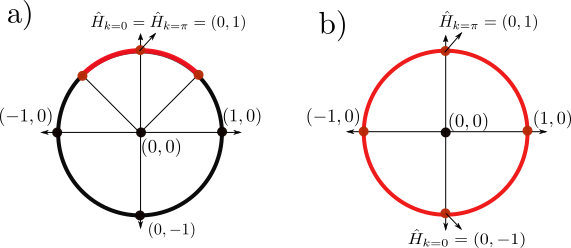
\includegraphics[scale=0.8]{IMAGES/Majorana/Topological.png}
    \label{fig:topological}
    \caption{ The following represents the path of $\hat{H}_k$ for the interval $[ -\pi, \pi ]$. a) Corresponds to the trivial phase. The resulting path can be homotopically deformed to a point. b) The non-trivial phase corresponds to a non-contractible loop around the unitary circle. \protect \Source{By the author}} 
\end{figure}

The mean idea behind this topological characterization relies in the adiabatic theorem.  In simple words, the adiabatic theorem says that a slow evolution of a gaped Hamiltonian will produce a smooth evolution of its ordered eigenstates. i.g The order of the eigenstates remains unchanged. \\

The keyword in the previous definition is "gaped". As we can observe in Figure \ref{fig:KitaevSpec} the phase transition occurs at $\frac{\mu}{2t}=1$. This is when the system transitions between a gapless and gaped Hamiltonians.  \\

The connection with topology comes from the fact that adiabatic evolutions can be understood as smooth deformations of the Hamiltonian. However since gapless Hamiltonians imply phase transitions, the theory defines the gapless points as holes (or forbidden points) in the phase space. Then characterizing the phase transitions in the Kitaev chain is mainly a topological problem where gaped Hamiltonians are holes in the topological space. In addition, the topological orders characterizing this transition will be Chern or Winding numbers. \\


% Though this connection between physics and topology is quite interesting, I will stop here because it is taking us out of our real discussion which is Majorana fermions.  You can find more information about this in ( \Jesus{add references}). 

% -----------------------Subsection: Non-abelian Statistics -------------
%\subsection{Non-abelian statistics}







% -----------------------Section: Modern and Experimental-------------
\section{Real implementations of Majorana Chains}
\Jesus{Here comes a summary of real models and implementations of Majorana chains. I am still thinking how to write this section. For now, I leave some ideas}

Although the Kitaev chain its just a toy model, 

The promise of finding the exotic Majorana particles that could bring new insights to quantum computing motivated the implementation of real models that could emulate the physics of a Kitaev chain. 

Spin is a major problem. A material with spin-orbit coupling is  the solution to this situation. \ref{fig:sipin-orbit} 

\begin{equation}
    H =\int\mbox{d}x\psi^{\dagger}\left(\frac{\partial^{2}}{2m\partial x^{2}}-\mu -i\alpha\sigma_{y}\partial x+h\sigma_{x}\right)\psi+\Delta\psi_{\downarrow}\psi_{\uparrow}+\Delta^{*}\psi_{\downarrow}\psi_{\uparrow},
    \label{eq:MajoranaChainHam}
\end{equation}




\begin{figure}[t]
\centering
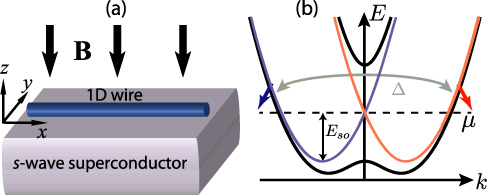
\includegraphics[scale=0.7]{IMAGES/Majorana/Mwire.png}

\caption{ \label{fig:spin-orbit} \protect\Source{\cite{alicea_new_2012}}}
\end{figure}

\begin{figure}[H]
\centering

     \subfloat[ \label{fig:exp1}]{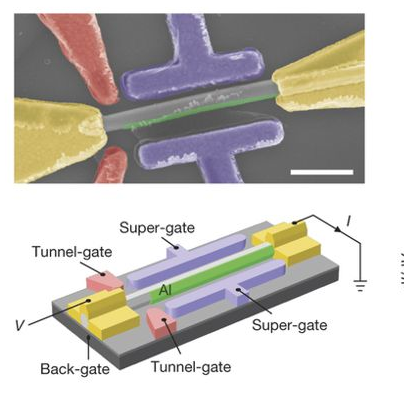
\includegraphics[scale=0.3]{IMAGES/Majorana/Exp.png}}  
     \subfloat[\label{fig:exp2}]{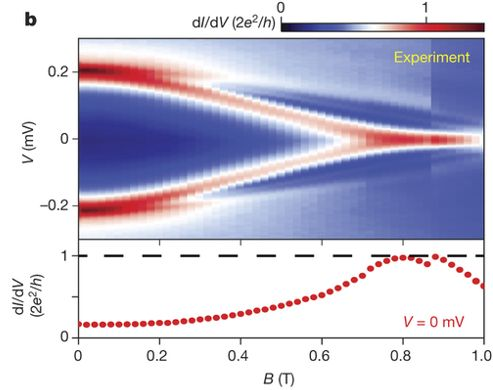
\includegraphics[scale=0.3]{IMAGES/Majorana/Exp2.png}}
\caption{ \label{ex}\protect\Source{\cite{zhang_quantized_2018}}}
\end{figure}


% -----------------------Leaking Majorana modes in quantum dots-------------

\section{Coupling Majorana Fermions to QDs}
\citeauthor{liu_detecting_2011} was one of the first to propose the possibility of using QDs in the pursuit of Majorana fermions . When a QD is attached to the end of a Majorana chain in the topological phase,  the Majorana Zero Mode at the end of the chain leaks inside the QD \cite{vernek_subtle_2014}. This produces a zero-bias conductance peak of half a quanta $\frac{e^{2}}{2h}$ through the dot. Using the ideas from \ref{chap: Methods} we can recreate this result. This will also allow us to probe our methods before going to the double-dot Majorana system in the following chapter. 

The Hamiltonian for Majorana-QD-lead hybrid system is is given by
\begin{equation}
    H=H_{QD-Lead}+H_{M-QD}+H_M.
\end{equation}
Where $H_{QD-Lead}$ is the Hamiltonian for the non-interacting Anderson model \eqref{eq:Anderson}, $H_M$ is the Hamiltonian of the Majorana chain and $H_{M-QD}$ represents the coupling between the QD and the Majorana Fermion at the boundary.

Now, the real question is how to define the coupling between the QD and the Majorana fermion. In fact, there are many ways to represent this interaction. One alternative is to replace in $H_{M}$ with the entire Kitaev chain hamiltonian \eqref{eq:kitaevHam} (or  even with the  Majorana chain \eqref{eq:MajoranaChainHam}) and then pick $H_{M-QD}$ as a simple coupling between the QD and the first site of the chain \cite{vernek_subtle_2014}.  A simpler approach is  to define an effective coupling with the Majorana operator at the edge of the Majorana chain. Since the Kitaev chain is spin-less, we choose to couple the Majorana to the spin-$\dw$ channel of the QD \footnote{An appropriate justification of this fact can be found in \cite{ruiz-tijerina_interaction_2015}} . Therefore, the Majorana fermion should be the superposition of the creation and annihilation operators of a spin $\dw$ particle $f_\dw$:

$$\gamma_1 := \frac{1}{\sqrt{2}} \left( f^\dagger_{\dw} + f_{\dw}\ \right) , \gamma_2 := \frac{1}{\sqrt{2}} \left( f^\dagger_{\dw} - f_{\dw} \right).$$

This makes possible to define an effective coupling between the Majorana Mode and the dot by attaching $\gamma_1$ with the spin-$\dw$ channel in the QD

%H_{TS} & = & 2\epsilon_{m}\gamma_{1}\gamma_{2}\nonumber \\
\begin{eqnarray}
H_{M-QD} & = &  t_1 \left(d_{\downarrow}^{\dagger}\gamma_{1}+\gamma_{1}d_{\downarrow}\right) 
% \\
% & = &  \sum_{i}t_{i} \left(d_{i\downarrow}^{\dagger}f^\dagger_{\dw} + 
% f_{\downarrow}d_{i\dw} +d_{i\downarrow}^{\dagger}f_{\dw}+
% +f_{\downarrow}^{\dagger} d_{i\downarrow}\right).
\label{eq:MajoranaCoupling}
\end{eqnarray}




% \begin{equation}
%     \omega\Green{A,B} =\delta_{A^{\dagger},B}+\Green{\left[A,H\right],B}
% \end{equation}

Then the coupling with the chain is given by 

\begin{eqnarray*}
H_{M} & = & \epsilon_{m}f_{\downarrow}^{\dagger}f_{\downarrow}\\
H_{M-QD}&=&\frac{t_1}{\sqrt{2}}d_{1\downarrow}^{\dagger}f_{\downarrow}+\frac{t_1^{*}}{\sqrt{2}}f_{\downarrow}^{\dagger}d_{1\downarrow}+\frac{t_1}{\sqrt{2}}d_{1\downarrow}^{\dagger}f_{\downarrow}^{\dagger}+\frac{t_1^{*}}{\sqrt{2}}f_{\downarrow}d_{1\downarrow}
\end{eqnarray*}

Finally we obtain the following hamiltonian

\begin{equation}
H =\sum_{k,\sigma}\left(\epsilon_1+\frac{U_1}{2}\right)d_{1\sigma}^{\dagger}d_{1\sigma}+ \frac{U}{2}(d_{1\sigma}^{\dagger}d_{1\sigma}-1)^{2} + t_1 \left(d_{1\downarrow}^{\dagger}\gamma_{1}+\gamma_{1}d_{1\downarrow}\right) + Vd^\dagger_{1\sigma}c_{k\sigma}+V^* c^\dagger_{k\sigma}d_{1\sigma}+ \epsilon_{m}f_{\downarrow}^{\dagger}f_{\downarrow}.
\label{eq:QD-Mham}
\end{equation}


The fidelity of this effective model has been discussed by \citet{ruiz-tijerina_interaction_2015}
concluding that the Majorana effective hamiltonian reproduces the
same results than the Kitaev chain model in the topological phase
(This statement is true even for more realistic models of the TS that
include Rashba spin-orbit interactions and a Zeeman field \citep{ruiz-tijerina_interaction_2015}
).\\


\subsection{Non-interacting QD coupled to a Majorana chain}

In the non-interacting case we can use the ballistic transport equations from \ref{sec:transport}.The green functions are then determined by the following set of linear equations. 




\begin{align}
    \left(\omega-\epsilon_{M}\right)\Green{f_{\downarrow},d_{1\downarrow}^{\dagger}}&=\left(\omega+\epsilon_{M}\right)\Green{f_{\downarrow}^{\dagger},d_{1\downarrow}^{\dagger}}=\frac{t^*_1}{\sqrt{2}}\left(\Green{d_{1\downarrow},d_{1\downarrow}^{\dagger}}-\Green{d_{1\downarrow}^{\dagger},d_{1\downarrow}^{\dagger}}\right)\\
    \left(\omega-\epsilon_{1}\right)\Green{d_{1\downarrow},d_{1\downarrow}^{\dagger}}&=1+\frac{t_1}{\sqrt{2}}t_{1}\Green{f_{\downarrow},d_{1\downarrow}^{\dagger}}+\frac{t_1}{\sqrt{2}}t_{1}\Green{f_{\downarrow}^{\dagger},d_{1\downarrow}^{\dagger}}+V_{1}\sum_{\mathbf{k}}\Green{c_{\mathbf{k\downarrow}},d_{1\downarrow}^{\dagger}}\\
    \left(\omega-\epsilon_{\mathbf{k}}\right)\Green{c_{\mathbf{k}},d_{1\downarrow}^{\dagger}}&=V_{1}^{*}\Green{d_{1\downarrow},d_{1\downarrow}^{\dagger}}\\
    \left(\omega+\epsilon_{1}\right)\Green{d_{1\downarrow}^{\dagger},d_{1\downarrow}^{\dagger}}&=-\frac{t_1}{\sqrt{2}}\Green{f_{\downarrow},d_{1\downarrow}^{\dagger}}-\frac{t_1}{\sqrt{2}}\Green{f_{\downarrow}^{\dagger},d_{1\downarrow}^{\dagger}}-V_{1}^{*}\sum_{\mathbf{k}}\Green{c_{\mathbf{k\downarrow}}^{\dagger},d_{1\downarrow}^{\dagger}}\\
    \left(\omega+\epsilon_{\mathbf{k}}\right)\Green{c^\dagger_{\mathbf{k}},d_{1\downarrow}^{\dagger}}&=-V_{1}^{*}\Green{d_{1\downarrow},d_{1\downarrow}^{\dagger}}
\end{align}

The graph representing these green functions is represented in \ref{fig:green-M-QD} a)  (Look \ref{sec:GraphMethod} for details). However using that $\left(\omega-\epsilon_{M}\right)\Green{f_{\downarrow},d_{1\downarrow}^{\dagger}}=\left(\omega+\epsilon_{M}\right)\Green{f_{\downarrow}^{\dagger},d_{1\downarrow}^{\dagger}}$ we can take
 $\Green{f_{\downarrow}^{\dagger},d_{1\downarrow}^{\dagger}}$ out of the equations getting the system in \ref{fig:green-M-QD} b) .  Using the graph algorithm from \ref{sec:Algorithm}  we proceed to pop out vertexes $c_k$ , $c_k^\dagger$ and $d_1^\dagger$ in that order. The result is the graph in figure \ref{fig:green-M-QD}.c) with 
 
 \begin{figure}[t]
    \centering
    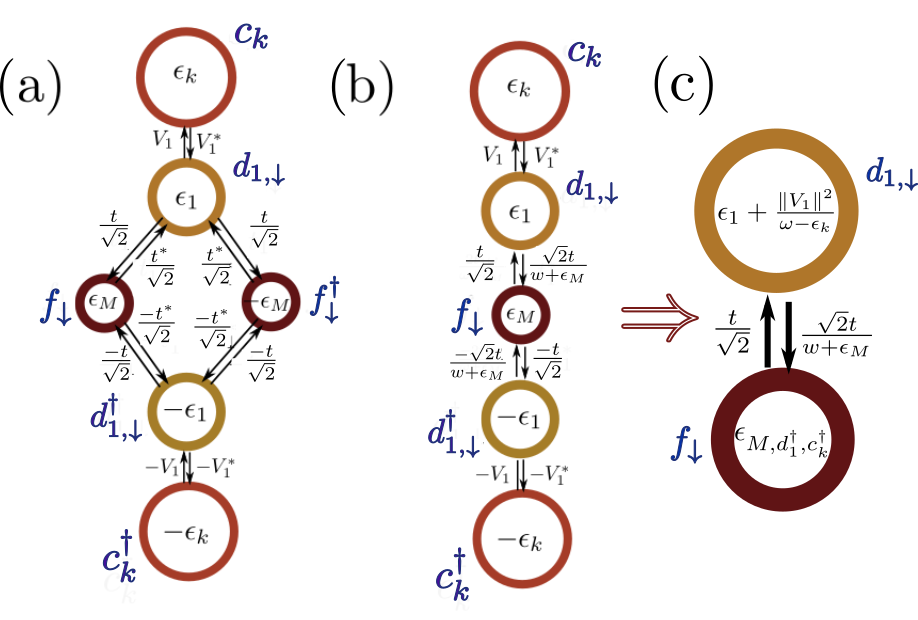
\includegraphics[scale=0.5]{IMAGES/Graphs/Grenn-Majorana.png}
    \caption{ Graph $\GM$ representing the transport equations.  \label{fig:green-M-QD} \protect\Source{By the author}}
\end{figure}
 
 \begin{equation}
    \epsilon_{M,d_1^\dagger,c^\dagger}= \epsilon_{M}+\frac{\omega}{\omega+\epsilon_{M}}\frac{\left\Vert t\right\Vert ^{2}}{\omega+\epsilon_{1}+\sum_{\mathbf{k}}\frac{V_{1}V_{1}^{*}}{\omega+\epsilon_{\mathbf{k}}}}.
\end{equation}
 
 We finally pop out $f_\dw$ to obtain 
 
\begin{equation}
    \Green{d_{1\downarrow},d_{1\downarrow}^{\dagger}}=\left[\omega-\epsilon_{1}-\sum_{\mathbf{k}}\frac{V_{1}V_{1}^{*}}{\omega-\epsilon_{1}}-\frac{\omega}{\omega+\epsilon_{M}}\frac{\left\Vert t\right\Vert ^{2}}{\omega -\epsilon_{M,d_1^\dagger,c^\dagger}}\right]^{-1}.
\end{equation}
Hence we just need the green function of $\GreenG{f_{\downarrow},f_{\downarrow}^{\dagger}}{\GM-d_{1}}$ removing $d_1$ out of the graph. This case is much simpler since $f_\downarrow$ is just attached to $d^\dagger_1$ . Thus we get
\begin{equation}
    \GreenG{f_{\downarrow},f_{\downarrow}^{\dagger}}{\GM-d_{1}}=\left[\omega-\epsilon_{M}-\frac{\omega}{\omega+\epsilon_{M}}\frac{\left\Vert t\right\Vert ^{2}}{\omega+\epsilon_{1}-\sum_{\mathbf{k}}\frac{V_{1}V_{1}^{*}}{\omega-\epsilon_{\mathbf{k}}}}\right]^{-1}.
\end{equation}

The only missing point in this equation is to replace $\sum \frac{V_1V^*_1}{\omega -\epsilon_k}= -i\Gamma_1$ as we already did in \ref{sec:GraphMethod}. Note that these computations are only for the spin-$\dw$ channel. The spin-$\up$ channel is even simpler since this channel is not coupled to the Majorana mode by convention. Hence it corresponds to the case of a single quantum dot coupled to a Lead.  The results for the DOS can be observed in \ref{fig:M1-Tot}. Each figure has an inset showing the model in the Majorana representation. The small blue and red balls are Majorana fermions just as the ones in figure \ref{fig:top.phases kitaev}. The Majorana at the edge of the  chain is represented by the isolated red ball connected to the QD (Figure \ref{fig:M1}). The other isolated blue ball in Figure \ref{fig:M1-em} represents the Majorana at the other edge which is connected to the sphere by the parameter $\epsilon$. 
\Jesus{Here comes the interpretation}
\begin{itemize}
    \item\textbf{Figure: \ref{fig:M1}}  The spin-$\up$ DOS shows the result when the Majorana is uncoupled, hence corresponding to a quantum dot coupled to a lead. When the Majorana is attached to the dot $t>0$ the DOS decays to the half. This robust signature 
    \item\textbf{Figure: \ref{fig:M1-e1}}
    \item\textbf{Figure: \ref{fig:M1-em}}
\end{itemize}



\begin{figure}[t]
     \centering
    \subfloat[Figure  \label{fig:M1}]{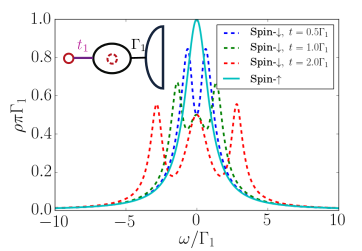
\includegraphics[scale=0.6]{IMAGES/Majorana/M1.png}}
     \subfloat[Figure \label{fig:M1-e1}]{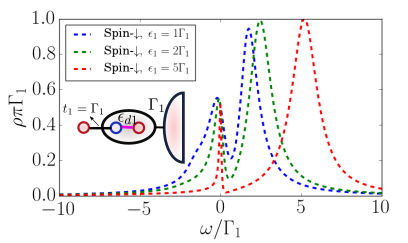
\includegraphics[scale=0.6]{IMAGES/Majorana/M1-e1.png}}  \\
    \subfloat[\label{fig:M1-em}]{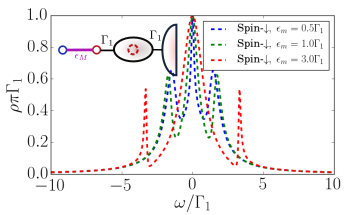
\includegraphics[scale=0.6]{IMAGES/Majorana/M1-eM.png}}
    
     \caption{Figure \label{fig:M1-Tot} ..\Jesus{I don't like the variables of  the c) plot. So I might change them soon}.  \protect\Source{ By the Author  }}
\end{figure}




\subsection{NRG: Kondo-Majorana physics}
In the interacting case the Kondo peak will appear at the fermi energy. In addition, the Majorana in the spin-$\dw$ channel will produce a peak at the fermi energy of Half of the amplitude of the Kondo peak (See \ref{fig:NRG-1M}). This will be our Majorana signature. 
\begin{figure}[H]
\centering
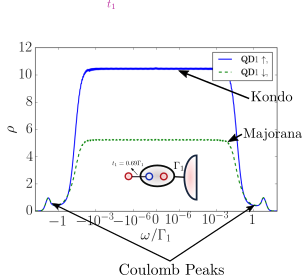
\includegraphics[scale=0.7]{IMAGES/Majorana/NRG.png}

\caption{ \Jesus{The units of this plot are a bit different than the NRG plots. That's mainly due to a problem I am having with the NRG plots. I will unify the format soon. } \label{fig:NRG-1M} \protect\Source{\cite{By the author.}}}
\end{figure}


 \citeauthor{ruiz-tijerina_interaction_2015}  proved that this effective coupling  is able to reproduce efficiently the results obtained when the Kitaev chain in the topological phase is attached to a single QD. 

% \begin{eqnarray*}
% H_{TS} & = & 2\epsilon_{m}f_{\downarrow}^{\dagger}f_{\downarrow}-\epsilon_{m}\\
% H_{int} & = & \sum_{i}\tilde{t_{i-}}d_{i\downarrow}^{\dagger}f_{\downarrow}+\tilde{t_{i-}}^{*}f_{\downarrow}^{\dagger}d_{i\downarrow}+\tilde{t_{i+}}d_{i\downarrow}^{\dagger}f_{\downarrow}^{\dagger}+\tilde{t_{i+}}^{*}f_{\downarrow}d_{i\downarrow}
% \end{eqnarray*}

% with $\tilde{t}_{i\pm}=\frac{1}{\sqrt{2}}\left(\left|t_{i1}\right|-i\left|t_{i1}\right|e^{i\phi_{i}}\right).$



% so that 

% \[
% \gamma_{1}=\frac{1}{\sqrt{2}}\left(f_{\downarrow}^{\dagger}+f_{\downarrow}\right)\ ,\gamma_{2}=\frac{1}{i\sqrt{2}}\left(f_{\downarrow}^{\dagger}-f_{\downarrow}\right).
% \]


% \begin{eqnarray}
% H_{TS} & = & 2\epsilon_{m}\gamma_{1}\gamma_{2}\nonumber \\
% H_{int} & = & \sum_{i}t_{i1}\left(d_{i\downarrow}^{\dagger}\gamma_{1}+\gamma_{1}d_{i\downarrow}\right)+it_{i2}\left(d_{i\downarrow}^{\dagger}\gamma_{2}+\gamma_{2}d_{i\downarrow}\right),\label{eq:Majorana-ham}
% \end{eqnarray}


% where $\gamma_{1,2}$are the two Majorana operators and$t_{i1,2}$
% are the hopping terms between the Majoranas and the QDs.




% A Majorana chain coupled to a QD can be studied using the methods described in chapter \ref{chap: Methods}






% % where $H_{d_{i}}$is the QD hamiltonian for dot $i$ \prettyref{eq:DotHam}
% % ,$t$ is the hopping term between both dots, $H_{int}$is the dot-TS
% % interaction and $H_{TS}$ is the TS-hamiltonian . In \citep{vernek_subtle_2014},
% % the TS is modeled as a Kitaev chain \citep{kitaev_unpaired_2001}
% % and $H_{int}$ is the hopping interaction between dots and chain 

% \begin{eqnarray}
% H_{TS} & = & -\sum_{j=1}^{N}\mu a_{j}^{\dagger}a_{j}+\sum_{j=1}^{N-1}\left[-t'(a_{j}^{\dagger}a_{i+1}+a_{j+1}^{\dagger}a_{j})+\Delta a_{j}a_{j+1}+\Delta^{*}a_{j+1}^{\dagger}a_{j}^{\dagger}\right]\nonumber \\
% H_{int} & = & \sum t_{i}d_{i\downarrow}^{\dagger}a_{1}+t_{i}^{*}a_{1}^{\dagger}d_{i\downarrow},\label{eq:Kitaev-dot}
% \end{eqnarray}


% where $a_{j}^{\dagger}$is the creation operator at site $j$ of the
% chain, $t'$ is the hopping term between consecutive sites, $\Delta$
% is the superconducting gap and $t_{i}$ is the hopping interaction
% between the dot $i$ and the first site of the chain. We also assume
% the dot only interact with spin-down $\downarrow$ operators in the
% chain. \\

% Using a Green's function approach on \prettyref{eq:Kitaev-dot} ,
% \citet{vernek_subtle_2014} concludes that the Majorana mode at the
% end of the chain leaks inside the QD when the TS is in the topological
% phase . This fact favors a more simple effective model that has been
% used in literature for simulation QD-TS interactions \citep{liu_detecting_2011,golub_kondo_2011,lee_kondo_2013}.
% The model consists in considering only the coupling between the dots
% and the Majorana modes that emerge in the topological phase. The resulting
% hamiltonian is 



% \[
% f_{\downarrow}^{\dagger}=\frac{1}{\sqrt{2}}\left(\gamma_{1}-i\gamma_{2}\right)\ ,\ f_{\downarrow}=\frac{1}{\sqrt{2}}\left(\gamma_{1}+i\gamma_{2}\right)
% \]


% so that 

% \[
% \gamma_{1}=\frac{1}{\sqrt{2}}\left(f_{\downarrow}^{\dagger}+f_{\downarrow}\right)\ ,\gamma_{2}=\frac{1}{i\sqrt{2}}\left(f_{\downarrow}^{\dagger}-f_{\downarrow}\right).
% \]


% Supposing $t_{i1}=\left|t_{i1}\right|$ and $t_{i2}=\left|t_{i2}\right|e^{i\phi_{i}}$
% to have a $\phi_{i}$-phase with respect to $t_{i1}$, we get to the
% following hamiltonian 



% \begin{eqnarray}
% H_{TS-2QDs} & = & H_{d_{i}}+\sum_{\sigma}\left(td_{1\sigma}^{\dagger}d_{2\sigma}+t^{*}d_{1\sigma}^{\dagger}d_{2\sigma}\right)\nonumber \\
%  &  & \ \enskip\ \enskip+\sum_{i}\left[\tilde{t_{i-}}d_{i\downarrow}^{\dagger}f_{\downarrow}+\tilde{t_{i-}}^{*}f_{\downarrow}^{\dagger}d_{i\downarrow}+\tilde{t_{i+}}d_{i\downarrow}^{\dagger}f_{\downarrow}^{\dagger}+\tilde{t_{i+}}^{*}f_{\downarrow}d_{i\downarrow}\right]+2\epsilon_{m}f_{\downarrow}^{\dagger}f_{\downarrow}-\epsilon_{m}.\label{eqFinalMJ-2QDs}
% \end{eqnarray}



% \chapter{Coupling a Double Quantum Dot with a Majoran Mode}
%--------------------------------------------------------------------------
\note{This section is still a bit disorganized since most of the results are new.   }
In this section we present the results for the NRG analysis of the Anderson model applied to the case of a Double Quantum Dot (DQD) attached to a Majorana mode (See \ref{fig:GeneralModel}). Extending the  Hamiltonian \eqref{eq:QD-Mham} to a coupling with a DQD we obtain the following general Hamiltonian:   

\begin{equation}
H =\sum_{i=1}^2\sum_{k,\sigma}\left(\epsilon_{i}+\frac{U_i}{2}\right)d_{\sigma}^{\dagger}d_{i\sigma}+ \frac{U_i}{2}(d_{i \sigma}^{\dagger}d_{i \sigma}-1)^{2} + t_i(\gamma d_{+,\dw}+d^\dagger_{+,\dw}\gamma) + V_id^\dagger_{i\sigma}c_{k\sigma}+V_i^* c^\dagger_{k\sigma}d_{i\sigma}.
\label{General model}
\end{equation}

\Jesus{I neglected $\epsilon_M$ in this case. Depending on the future NRG results I will choose to add it or leave it that way. }


\begin{figure*}[h]
\centering
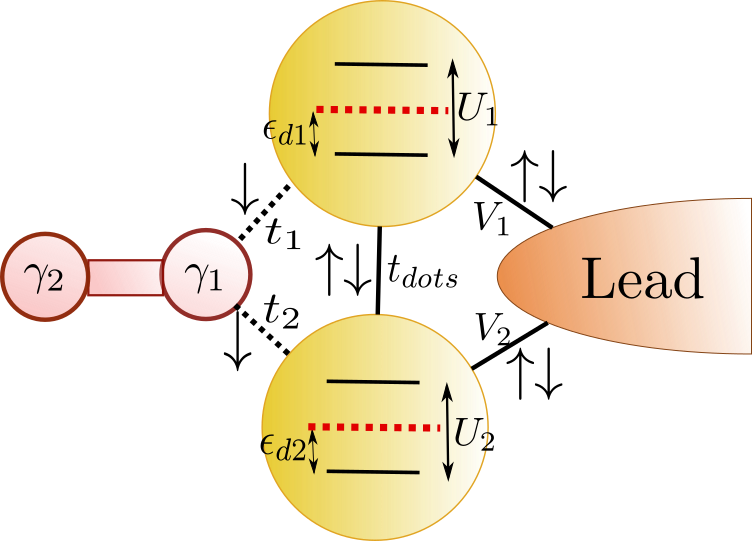
\includegraphics[scale=0.4]{IMAGES/GenModel.png}
\caption{\label{fig:GeneralModel}General model.} 
\end{figure*}



In order to understand the physical properties of this model, we probed a set of thought processes. The main variable in this analysis is the Density of States.  We  will observe its evolution on both QDs under the tuning of the model parameters such as:
\begin{enumerate}
    \item Hopping between Dots and Majorana Mode ($t_1 , t_2$). 
    \item Gate voltage ($\ed{1} , \ed{2} $)
    \item Inter dot coupling ($t_{dots}$)
\end{enumerate}


These processes intend to show whether it is possible to "manipulate" the majorana modes inside the dots by tuning the established parameters.The processes we found to show interesting physics are summarized in table. 
\begin{figure*}[h]
\centering
\includegraphics[scale=0.4]{IMAGES/Mo}
\caption{\label{fig:GeneralModel}General model.} 
\end{figure*}

\begin{figure*}[h]
\centering
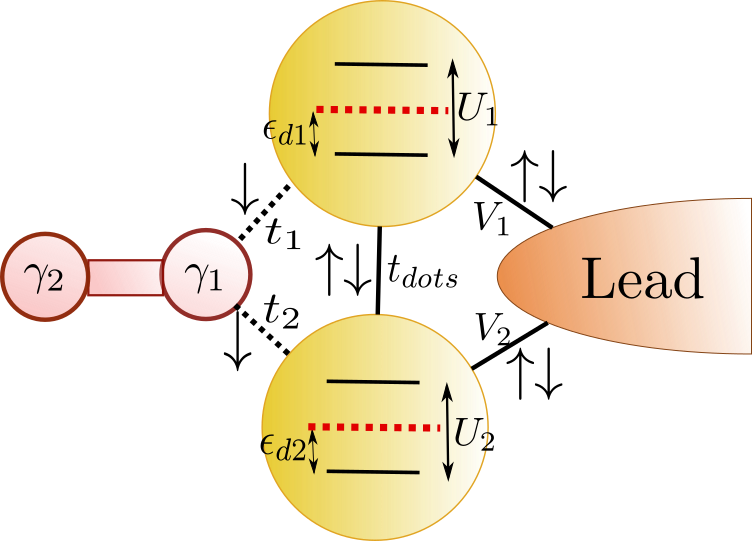
\includegraphics[scale=0.4]{IMAGES/GenModel.png}
\caption{\label{fig:GeneralModel}General model.} 
\end{figure*}


\newpage
\newpage



\section{Attaching the Majorana mode to the DQD (Tuning $t_1=t_2$) \label{sec:t1=t2}}

\textbf{Parameters:}

$$\Gamma \sim 2.83*10^{-2}D, t_{dots}=0 , U_{1,2} = -2\ed{1,2} = 0.5$$
$$t_1=t_2 \in [0\  ,\  2.5*10^{-2}D]$$

\begin{figure}[hbt]
\centering
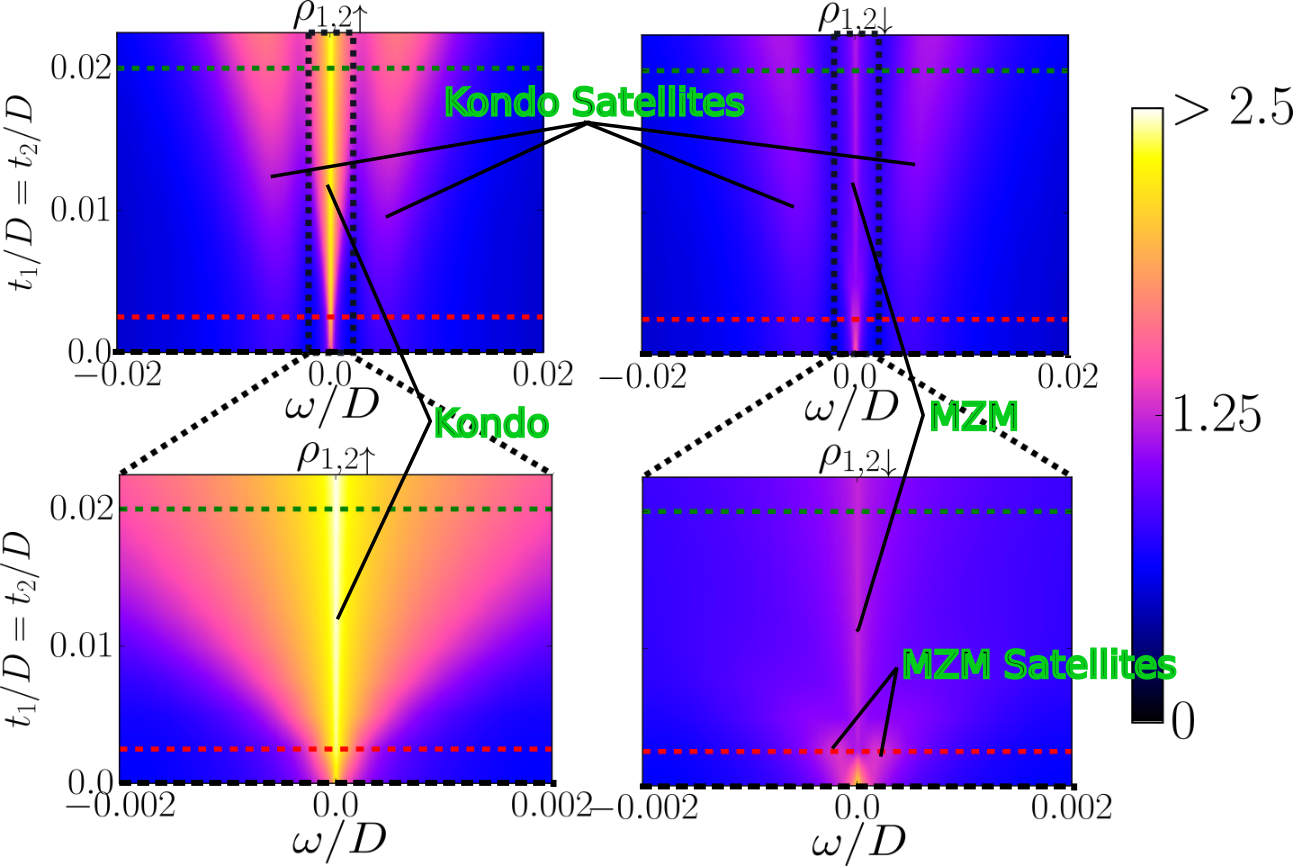
\includegraphics[scale=0.35]{IMAGES/t1=t2/2D.png}
\caption{\label{fig:2D/Shift_t1=t2} Evolution of the DOS of both QDs through $t_1 = t_2$ tuning. UP: Energy scale $\omega \sim 10^{-2}D$. DOWN: Energy scale $\omega \sim 10^{-3}D$. LEFT: Spin $\up$. RIGHT: Spin $\dw$.}
\end{figure}



The first process consists in attaching the Majorana mode to both Quantum Dots symmetrically. For this, we scale up the coupling parameter $t_1=t_2$ from $0$ (Decoupled) to $0.02$ (Completely coupled).The other parameters where chosen with an equilibrium between the dot energy and Coulomb repulsion $(\ed{1,2}=-\frac{U_{1,2}}{2})$  and  without inter-dot coupling $t_{dots}=0$. These circumstances guarantee that the system preserves Particle Hole Symmetry (PHS). Thus the Density of States (DOS) of particles and holes remains equal at all instances $(\rho(-\omega) = \rho(\omega))$. \\

\begin{figure}[hbt]
\centering
\includegraphics[scale=0.35]{IMAGES/t1=t2/LogPlot.png}
\caption{\label{fig:t1=t2/logplot} Density of states at each QD of the horizontal dashed cuts in \ref{fig:2D/Shift_t1=t2}. The energy is in logarithmic scale.  For $t_1=t_2>0$ spin-$\up$ and spin-$\dw$ DOS split near the order of $\vert \omega \vert \sim t_1,2 $. At the Fermi energy $(\omega =0)$  $\rho_\up = 2\rho_\dw$ due to the presence of the MZM in both QDs. }
\end{figure}

In the case where the majorana is detached from the DQD $(t_1 =t_2 = 0)$, the system favors the appearance of a three-peak at low energies as it is shown in \ref{fig:t1=t2/logplot} . The central peak is produced only by the Kondo effect and the two other satellite peaks are the result of a strong correlation between both dots caused by the indirect exchange of quantum states through the Lead \ref{sec:DoublePeak}. \\

Once the MZM the spin-$\up$ and spin-$\dw$ DOS split at low energies due to the new spin-$\dw$ transport channel through the Majorana mode. The spin-$\dw$ DOS at the Fermi energy ($\omega =0$) decays to the half of the spin-$\up$ DOS $\rho_\dw = \frac{\rho_\up}{2} $. By symmetry in the dot parameters this event occurs equally for both QDs. We adopt this fact as a Majorana signature. Hence we obtain that the MZM leaks inside both quantum dots. 

There is also an additional effect caused by the indirect exchange between the QDs through the Majorana mode . The consequences of this effect depend on the energy range of the majorana couplings $t_1=t_2$.  : 
\begin{enumerate}
    \item If $t_1=t_2 \ll \Gamma $ two more satellites are formed at very low energies ($\sim t_1$) in the spin-$\dw$ DOS (See  \ref{fig:2D/Shift_t1=t2} Spin-down $\omega \sim 10^{-3}D$ ). (See  \ref{fig:2D/Shift_t1=t2} Spin $\up$, $\omega \sim 10^{-3}D$ ).
    \item If $t_1=t_2 \sim \Gamma$ , the MZM contributes to the the growth of the spin-up satellites in the DOS. This effect produces the splitting between the spin-up and spin-down DOS.   (See  \ref{fig:2D/Shift_t1=t2} Spin-$\dw$, $\omega \sim 10^{-2}D$).
\end{enumerate}








\iffalse
At low energies $(\omega/D \sim 10^{-2})$ \ref{fig:2D/Shift_t1=t2} shows the emergence of a 3-peak in the DOS close to the Fermi energy. This 3-peak is formed by a central peak defined by the Kondo (spin $\up$) and the Majorana (spin $\dw$) peaks. The other two peaks are generated by an indirect exchange of the states between the quantum dots through the leads (SEE ABSTRACT). At even lower energies $(\omega/D \sim 10^{-4})$ it is possible to appreciate the emergence of another 3-peak in the spin down DOS which is present only for small values of the Majorana coupling constants $t_1 = t_2 \ll 0.01D$ (See  \ref{fig:t1=t2/logplot}). These sided peaks are caused by the indirect exchange between both dots through the Majorana Mode. When the Majorana couplings achieve the same order of the dot-lead coupling $\Gamma$ $(t_1 = t_2 \sim  0.01D)$ both sided peaks are merged causing the extinction of the majorana side-peaks and the increase of the indirect exchange peaks at $(\omega/D \sim 10^{-2})$. 

\begin{figure}[H]
\centering
\includegraphics[scale=0.4]{Plots/MSig/Shift_t1=t2.png}
\caption{\label{fig:MSig/Shift_t1=t2} Relation between the Zero-peaks at the fermi level. The Majorana signature is related to $\frac{\rho_\up(0)}{\rho_\up(0)}=2$.}
\end{figure}
\fi




















%--------------------------------------------------------------------

\section{Transferring the MZM through gate voltage shifting $\ed{2}$. \label{sec:e2}}

\textbf{Parameters:}

$$\Gamma \sim 2.83*10^{-2}D, t_{dots}=0 , U_{1,2} = -2\ed{1} = 0.5 , t_1=t_2=0.0025$$
$$\ed{2} \in [-0.25 \  , -0.05]$$

This process starts with the DQD coupled symmetrically  to the Majorana mode, just as in \ref{sec:t1=t2}. The idea of this process is to break PHS by increasing the energy of the second QD $\ed{2}$. This procedure should induce the Majorana to tunnel only into the first dot. 


\begin{figure}[h]
\centering
\includegraphics[scale=0.35]{IMAGES/ed2/2D.png}
\caption{\label{fig:2D/Shift_ed2} Evolution of the DOS of both QDs through the $\ed{2}$ tuning. UP: QD1. DOWN: QD2. LEFT: Spin $\up$. RIGHT: Spin $\dw$.}
\end{figure}


In \ref{fig:2D/Shift_ed2} we observe that both, the Kondo and the MZM peaks are preserved in the first QD as well as the majorana signature (See \ref{fig:ed2/Fermi}) when $\ed{2}$ is scaled up to $-0.1$.  However,  PHS breaking will favor the growth of the spin-$\up$ hole $(w>0)$  satellite and the spin-$\dw$ particle $(w<0)$ satellite.




In the second QD the DOS increases abruptly for both spins.The majorana signature is rapidly when  lost . Hence, with this set-up it is actually possible to induce the Majorana to preferably tunnel QD1 in despite of QD2.  \\
\begin{figure}[H]
\centering
\includegraphics[scale=0.3]{IMAGES/ed2/Fermi.png}
\caption{\label{fig:ed2/Fermi} As described in \ref{sec:t1=t2} the relation $\frac{\rho_\up(0)}{\rho_\up(0)}=2$ constitutes a Majorana Signature . This picture evaluates shows the evolution of the relation $\frac{\rho_\up(0)}{\rho_\up(0)}$ for both QDs. While QD2 losses rapidly the Majorana signature, QD1 maintains it till $\ed{2}\sim -0.1$.}
\end{figure}


\newpage


%---------------------------------------------------------------------------

\section{Particle-Hole symmetric shifting of $\ed{2}=\frac{U}{2}$.}

\begin{figure*}[h]
\centering
\includegraphics[scale=0.2]{Plots/Model/Majorana-2QD.eps}
\caption{\label{fig:Mod/PHS-Shift_e2.png}$U_{1}=-2\ep_{d1}=0.5$, $\Gamma_{1}=\Gamma_{2}$,
$t_{1}=t_2=0.02$. Variable $\ep_{d2} =\frac{U_{2}}{2}$}
\end{figure*}
\begin{figure}[hbt]
\centering
\includegraphics[scale=0.38]{Plots/DOS/PHS-Shift_e2.png}
\caption{\label{fig:DOS/PHS-Shift_e2.png} Evolution of the QDs' DOS for the model in \ref{fig:Mod/PHS-Shift_e2.png} }
\end{figure}
We start again with the symmetric model with both QDs coupled to the Majorana mode, but this time the evolution is performed over $\ep_2=\frac{U}{2}$, such that the model is always Particle-Hole symmetric. This situation is very different from the previous model (\ref{sec:e2}) since the decaying of $U2$ 
equalizes the effect of increasing the dot energy. In \ref{fig:DOS/PHS-Shift_e2.png} we observe that the DOS of QD2 increases while the QD1's DOS decreases, just as it happened in \ref{sec:e2} . However, the Majorana signature remains at $2$ for both dots (See \ref{fig:MSig/PHS-Shift_e2}), meaning that the Majorana is not preferably induced to tunnel to any QD despite the lose of symmetry in the dot energy.

\begin{figure}[hbt]
\centering
\includegraphics[scale=0.4]{Plots/MSig/PHS-Shift_e2.png}
\caption{\label{fig:MSig/PHS-Shift_e2} Relation between the spin up-down Zero-peaks at the Fermi level. The Majorana signature is related to $\frac{\rho_\up(0)}{\rho_\up(0)}=2$.}
\end{figure}

%---------------------------------------------------------------------------
\section{Shifting $t_2$}

%$U_{1}=U_{2}=-2\epsilon_{d1}=-2\epsilon_{d2}=0.5$, %$\Gamma_{1}=\Gamma_{2}$,
%$t_{1}=0.02$

\begin{figure*}[h]
\centering
\includegraphics[scale=0.2]{Plots/Model/Majorana-1QD.eps}
\caption{\label{fig:Mod/Shift_t2}$U_{1}=U_{2}=-2\ep_{d1}=-2\epsilon_{d2}=0.5$, $\Gamma_{1}=\Gamma_{2}$,
$t_{1}=0.02$. Variable $t_2$}
\end{figure*}


\begin{figure}[hbt]
\centering
\includegraphics[scale=0.38]{Plots/2D/Shift_t2D1.png}
\caption{\label{fig:DOS/Shift_t2D1} Evolution of the DOS in the first QD }
\end{figure}
\begin{figure}[hbt]
\centering
\includegraphics[scale=0.38]{Plots/2D/Shift_t2D2.png}
\caption{\label{fig:DOS/Shift_t2D2} Evolution of the DOS in the Second QD}
\end{figure}



\iffalse
\begin{figure}[hbt]
\centering
\includegraphics[scale=0.38]{Plots/DOS/Shift_t2.png}
\caption{\label{fig:DOS/Shift_t2} Evolution of the QDs' DOS for the procedure in \ref{fig:Mod/Shift_t2} }
\end{figure}
\fi
 In \ref{fig:DOS/Shift_t2D1} and \ref{fig:DOS/Shift_t2D1} we observe the evolution of DOS in the case where the second dot is smoothly connected to the Majorana, which is already attached to the first dot. The hopping parameter $t_2$ scales up to $0.015D$ where the model reaches the symmetry $t_2 = t_1$. The figures show that increasing $t_2$ leads to a drop in the DOS of QD1 while the DOS in QD2 is increased. In addition, the single peak in the first dot transforms into a three-peak due to the Majorana interference with the second dot. In \ref{fig:MSig/Shift_t2} we also observe that the reason between the zero up-down DOS  $\left(\frac{\rho_\up(0)}{\rho_\up(0)}\right)$ smoothly scales up to $2$ in QD2. At $t_2 =0.02$, when the  is completely symmetric, the Majorana signature appears in both quantum dots. Note that the relation $\frac{\rho_\up(0)}{\rho_\up(0)}$  is already close to $2$ at $t_2=0$. This implies that the second dot "feels" the Majorana even when it is not directly connected to the Majorana mode. 





 States (DOS). The method used to compute the DOS is the Density Matrix numerical renormalization Group (DM-NRG). A complete description of this algorithm will be given in the following sections.  \\

% For now, we proceed to describe how the NRG is applied to solve the Anderson model in a QD:\\

% \Jesus{I still need to do a long revision to this section. Probably I will send most of the computations to the abstract and leave a summary of NRG and its advantages in the main text.}







%\begin{figure}[h]
%\centering
%\includegraphics[scale=0.5]{IMAGES/NRGchain.png}\caption{\label{FigNRG-chain} Chain-Hamiltonian describing the Anderson model.
%The chain starts at the initial dot hamiltonian $H_{d}$. The $f_{m}^{\dagger}$'s
%are the creation operators at the $n^{\mbox{th}}$-site of the chain.
%The $\xi_{n}$'s describe the magnitude of the interaction between
%consecutive sites. }
%\end{figure}




\subsection{Iterative diagonalization in a single QD attached to a metallic lead \label{subsec:QD-Diag} }

Now that we have an iterative representation of the Anderson Model
Hamiltonian \eqref{eq:Newchain-Hamiltonian}, we will describe how the NRG code works for a QD attached to a lead. We start with the dot Hamiltonian.

\begin{equation}
H_{d}=\frac{1}{D}\left(\epsilon+\frac{U}{2}\right)d_{\sigma}^{\dagger}d_{\sigma}+\frac{U}{2D}(d_{\sigma}^{\dagger}d_{\sigma}-1)^{2}.\label{eq:DotHam}
\end{equation}


\noindent Now observe that Hamiltonian \eqref{eq:DotHam} is already in the
diagonal form for the basis $\left\{ \vert\uparrow\!\downarrow\rangle,\vert\uparrow\rangle,\vert\downarrow\rangle,\vert0\rangle\right\} $
\[
H_{d}=\frac{1}{D}\left[\begin{array}{cccc}
2\epsilon+\frac{3U}{2} & 0 & 0 & 0\\
0 & \epsilon+\frac{U}{2} & 0 & 0\\
0 & 0 & \epsilon+\frac{U}{2} & 0\\
0 & 0 & 0 & \frac{U}{2}
\end{array}\right].
\]


Lets define $H_{-1} := \frac{2 H_d \Lambda^{-1/2}}{1+\Lambda^{-1}}$ as in \ref{eq:H-1}. It is convenient here to define unit-less variables $\epsilon' =\frac{2\epsilon \Lambda^{-1/2}}{D(1+\Lambda^{-1})}, U'= \frac{2U\Lambda^{-1/2}}{D(1+\Lambda^{-1})}$ and $\Gamma':=\sqrt{\frac{2\Gamma}{\pi D}}$. Then adding the first site of the Wilson's chain interaction to $H_{d}$ we obtain a new Hamiltonian of the form 

\begin{equation}
H_{0}=\Lambda^{\frac{1}{2}}H_{-1}+\Gamma'\left(d_{\sigma}^{\dagger}f_{0\sigma}+f_{0\sigma}^{\dagger}d_{\sigma}\right).\label{eq:H0fromH-1}
\end{equation}



The Hilbert space for this mew Hamiltonian must be extended to include
the $4$ degrees of freedom of the $f_{0\sigma}^{\dagger}$ particles,
which are given by $\left\{ \vert\uparrow\!\downarrow\rangle,\vert\uparrow\rangle,\vert\downarrow\rangle,\vert0\rangle\right\} $.
Therefore, the total Hilbert space for $H_{0}$ is given by a base
of the form 
\[
\vert s_{1}\rangle\vert s_{2}\rangle:=\vert s_{1}\rangle\otimes\vert s_{2}\rangle\mbox{ with }\vert s_{i}\rangle\in\left\{ \vert\uparrow\!\downarrow\rangle,\vert\uparrow\rangle,\vert\downarrow\rangle,\vert0\rangle\right\} .
\]


\noindent We obtain an space of dimension $4\times4=16.$ Now, before adventuring
to write the Hamiltonian for $H_{0}$ as a $16\times16$-matrix note
that $H_{-1}$ preserves the total particle number $\mathcal{N}$ and the total spin $S$. We can associate each state to one of these symmetries as 

\begin{align}
\vert \uparrow\downarrow\rangle\longrightarrow\vert \mathcal{N}=2,S=0\rangle\ ,& \ \vert0\rangle\longrightarrow\vert \mathcal{N}=0,S=0\rangle \\ 
\vert \uparrow\rangle\longrightarrow\vert \mathcal{N}=1,S=\frac{1}{2}\rangle\ ,& \ \vert \downarrow \rangle\longrightarrow\vert \mathcal{N}=1,S=\frac{-1}{2}\rangle.
\end{align}

The propagation rule for the symmetry is defined with the following identity 
\begin{equation}
  \vert \mathcal{N}_{1},S_{1}\rangle\otimes\vert \mathcal{N}_{2},S_{2}\rangle\subset\vert \mathcal{N}_{1}+\mathcal{N}_{2},S_{1}+S_{2}\rangle \label{eq:PropRuleQD}
\end{equation} 
  

 \noindent Then we can use  $\mathcal{N}$ and $S$ as quantum numbers to generate the the block structure of $H_{0}$ . We will observe that the terms in the diagonal will correspond to the eigenvalues of $H_{-1}$ for the first space. The non-diagonal terms are the result of the hopping interactions with the first site. 

\begin{multicols}{2}

$H_{\mathcal{N}=0,S=0}:$
\[
\begin{array}{c}
\vert0\rangle\vert0\rangle\rightarrow\end{array}\begin{array}{c}
\left[\frac{U'}{2}\right]\end{array}
\]


$H_{\mathcal{N}=4,S=0}:$
\[
\begin{array}{c}
\vert\uparrow\!\downarrow\rangle\vert\uparrow\!\downarrow\rangle\rightarrow\end{array}\begin{array}{c}
\left[2\epsilon'+\frac{3U'}{2}\right]\end{array}
\]


\end{multicols}

\begin{multicols}{2}

$H_{\mathcal{N}=1,S=\frac{1}{2}}:$
\[
\begin{array}{c}
\vert\uparrow\rangle\vert0\rangle\rightarrow\\
\vert0\rangle\vert\uparrow\rangle\rightarrow
\end{array}\left[\begin{array}{cc}
\epsilon'+\frac{U'}{2} & \Gamma'\\
\Gamma' & \frac{U'}{2}
\end{array}\right]
\]


$H_{\mathcal{N}=1,S=\frac{-1}{2}}:$
\[
\begin{array}{c}
\vert\downarrow\rangle\vert0\rangle\rightarrow\\
\vert0\rangle\vert\downarrow\rangle\rightarrow
\end{array}\left[\begin{array}{cc}
\epsilon'+\frac{U'}{2} & \Gamma'\\
\Gamma' & \frac{U'}{2}
\end{array}\right]
\]


\end{multicols}

\begin{multicols}{2}

$H_{\mathcal{N}=2,S=-1}:$
\[
\begin{array}{c}
\vert\downarrow\rangle\vert\downarrow\rangle\rightarrow\end{array}\begin{array}{c}
\left[\epsilon'+\frac{U'}{2}\right]\end{array}
\]


$H_{\mathcal{N}=2,S=1}:$
\[
\begin{array}{c}
\vert\uparrow\rangle\vert\uparrow\rangle\rightarrow\end{array}\begin{array}{c}
\left[\epsilon'+\frac{U'}{2}\right]\end{array}
\]


\end{multicols}


$H_{\mathcal{N}=2,S=0}:$
\[
\begin{array}{c}
\vert\uparrow\!\downarrow\rangle\vert0\rangle\rightarrow\\
\vert\uparrow\rangle\vert\downarrow\rangle\rightarrow\\
\vert\downarrow\rangle\vert\uparrow\rangle\rightarrow\\
\vert0\rangle\vert\uparrow\!\downarrow\rangle\rightarrow
\end{array}\left[\begin{array}{cccc}
2\epsilon'+\frac{3U'}{2} & \Gamma' & -\Gamma' & 0\\
\Gamma' & \epsilon'+\frac{U'}{2} & 0 & \Gamma'\\
-\Gamma' & 0 & \epsilon'+\frac{U'}{2} & -\Gamma'\\
0 & \Gamma' & -\Gamma' & \frac{U'}{2}
\end{array}\right]
\]


\begin{multicols}{2}

$H_{\mathcal{N}=3,S=\frac{1}{2}}:$
\[
\begin{array}{c}
\vert\uparrow\!\downarrow\rangle\vert\uparrow\rangle\rightarrow\\
\vert\uparrow\rangle\vert\uparrow\!\downarrow\rangle\rightarrow
\end{array}\left[\begin{array}{cc}
\epsilon'+\frac{U'}{2} & -\Gamma'\\
-\Gamma' & \frac{U'}{2}
\end{array}\right]
\]


$H_{\mathcal{N}=3,S=\frac{-1}{2}}:$
\[
\begin{array}{c}
\vert\uparrow\!\downarrow\rangle\vert\downarrow\rangle\rightarrow\\
\vert\downarrow\rangle\vert\uparrow\!\downarrow\rangle\rightarrow
\end{array}\left[\begin{array}{cc}
\epsilon'+\frac{U'}{2} & -\Gamma'\\
-\Gamma' & \frac{U'}{2}
\end{array}\right]
\]


\end{multicols}

\begin{figure}[t]
	\subfloat[$N$ takes only even values]{\includegraphics[scale=0.5]{IMAGES/even.png}}\subfloat[$N$ run only through odd values]{\includegraphics[scale=0.5]{IMAGES/odd.png}}\caption{\label{Fig-Dot-Spectrum} Evolution of the QD-spectrum vs number of
	iterations of the code for $U'=0.5,\ \ep'=-0.25,\ \Gamma=2.82\times10^{-2}.$ }
\end{figure}

The next step would be to diagonalize $H_{0}$ by blocks $(H_{\mathcal{N},S})$ and then including the next place in the chain. The following Hamiltonians are generated in the same way from equation \eqref{eq:NRG-Renormalization}. The symmetries of the new states can be obtained from the propagation rule \eqref{eq:PropRuleQD}. When the number of states surpasses the 1000 states, the code will automatically cutoff the higher energy states. However it is important that a Block is not divided in this cutting, since it could break the preserved symmetry. 

Finally, the spectrum for $\Lambda = 2.5$ takes the 'spaghetti' form in \ref{Fig-Dot-Spectrum}.  Note that before $N=30$, the low-energy contributions generate significant changes in the energy levels.  However, the stable spectrum after the step $N=30$ is a signature that the code has converged. As we previously declared, it is not $\mathcal{T}$ but $\mathcal{T}^2$ the transformation that has fixed points, which explains why it was necessary to plot the even and the odd spectrum separately.

% The resulting eigenvectors will be characterized by both quantum numbers
% so that we can write them in the form $\vert N,S,i\rangle$ with $i$
% taking as many values as the degeneracy of its block. For higher values of $N$,

% We now proceed by induction supposing that for each $N$ the Hamiltonian $H_{N}$ is already diagonalized and the eigenvectors are organized in states with labels $\vert N,S,i\rangle.$ The next step will be to add the $4$-Hilbert space corresponding to $f_{N+1,\sigma}$ organized the eigenvectors according to the quantum numbers $\vert N',S',i\rangle$ and proceed to diagonalize by blocks the new Hamiltonian. Apart of it, the code must have a cutoff to the number of states. \\

At the end of the NRG code, we obtain a complete list of the spectrum $(E_{i, N})$ and the eigenstates $(\vert i , N \rangle)$ of the Hamiltonian at each step $N$ of the chain ( See \ref{Fig-Dot-Spectrum}). It is important to keep all of these states since each one of them represents different thermodynamic regimes of the system. While the site $N=1$ represents the physics of the system relevant at temperatures around $\frac{D \Lambda^{-1}}{K_B }$, the site $N=30$ shows the low energy contributions at $T \sim \frac{D \Lambda^{-30}}{K_B }$ where the ground state is strongly correlated. Furthermore, the states at low temperatures are entangled with the higher energy states. We need to take this into account to extract dynamical quantities of the system, which is the objective of the following section. 

\subsection{The Density Matrix Renormalization Group (DM-NRG) \label{subsec:DM-NRG}}
The NRG codes allows us to compute several thermodynamic quantities such as the entropy $S$, the free energy and the partition function $Z(\beta)$. In addition, we can compute the spin magnetization or dynamical quantities such  the density of states, the magnetic susceptibility and the conductivity. To perform this we can use the spectrum obtained in the NRG code to define the Boltzman distribution of the system. Then we apply the usual methods of statistical mechanics.  

% It is necessary to embed NRG with the faculty to compute these operators at each step $N$ of the code. {} 

In this thesis we will focus in computing the density of states at the impurity (QD). For this, let $\vert j\rangle$ and $\vert q \rangle$ label a base of eigenstates of the Hamiltonian $H$. Now recall the definition of the retarded green function \eqref{eq:TempGreen}

\begin{align}
G_{d,d^{\dagger}}(t)&=\theta(t)\left\langle \{ d(t)d^{\dagger}(0) \} \right\rangle \\ \label{eq:MeanGreen}
&=\theta(t)\left\langle \left[e^{\frac{i}{\hbar}Ht}de^{-\frac{i}{\hbar}Ht}d^{\dagger}\right]\right\rangle +\theta(-t)\left\langle \left[d^{\dagger}e^{\frac{i}{\hbar}Ht}de^{\frac{-i}{\hbar}Ht}\right]\right\rangle \\
&=\theta(t)\sum_{\vert j\rangle,\vert q\rangle}p_{j}\langle j\vert e^{\frac{i}{\hbar}Ht}d\vert q\rangle\langle q\vert e^{-\frac{i}{\hbar}Ht}d^{\dagger}\vert j\rangle+\theta(-t)\sum_{\vert j\rangle,\vert q\rangle}p_{q}\langle q\vert d^{\dagger}e^{\frac{i}{\hbar}Ht}\vert j\rangle\langle j\vert de^{-\frac{i}{\hbar}Ht}\vert q\rangle\\
&=\theta(t)\sum_{\vert j\rangle,\vert q\rangle}p_{j}e^{\frac{-i}{\hbar}t\left(E_{j}-E_{q}\right)}\left\Vert \langle j\vert d\vert q\rangle\right\Vert ^{2}+\theta(-t)\sum_{\vert j\rangle,\vert q\rangle}p_{q}e^{\frac{i}{\hbar}t\left(E_{j}-E_{q}\right)}\left\Vert \langle j\vert d\vert q\rangle\right\Vert ^{2}
\end{align}

\noindent Where $p_{j}:=\frac{e^{-\beta E_{j}}}{Z(\beta)}$ defines the Boltzmann probability of the eigenstate $\vert j\rangle$ according to Hamiltonian $H$. 

It is known that the Fourier transform of an expression of the form ${\displaystyle e^{-ax}\theta(x)}$ is $\frac{1}{\omega+is-a}$. Then the Green function in the energy domain is 
\begin{equation}
\Green{d,d^{\dagger}}=\frac{1}{Z(\beta)}\sum_{\vert j\rangle,\vert q\rangle}{\displaystyle \frac{e^{-\beta E_{j}}+e^{-\beta E_{q}}}{\omega+is-E_{j}+E_{q}}}\left\Vert \langle j\vert d\vert q\rangle\right\Vert ^{2}
. \label{eq:greenT}
\end{equation}

\noindent From the imaginary part of \eqref{eq:greenT} we obtain a formula for the spectral density in terms of the eigenstates and energies of the Hamiltonian 
\begin{equation}
\rho_{d}=\frac{1}{Z(\beta)}\sum_{\vert j\rangle,\vert q\rangle}{\displaystyle \left(e^{-\beta E_{j}}+e^{-\beta E_{q}} \right) \delta\left(\omega-E_{j}+E_{q} \right) } \left\Vert \langle j\vert d\vert q\rangle \right\Vert^{2}. \label{eq:DOSeigenstates}
\end{equation}

\noindent This new expression for the DOS can be integrated into  the NRG code in different ways . A first method created by Costi \textit{et al.} consists in computing \eqref{eq:DOSeigenstates} with the eigenstates of each shell Hamiltonian $H_N$  \cite{costi_transport_1994}. It is necessary to take into account that the operator $ d$ is constantly rotating after each diagonalization procedure, which produces different representations at each shell Hamiltonian basis. Then, an important part of Costi's algorithm is to obtain these new representations of $d$ at the $H_N$-basis $(\langle j\vert d\vert q\rangle\Vert_N)$ recursively starting from an input representation $\langle j\vert d\vert q\rangle\Vert_{N=0}$.

Although Costi's method predicts accurately the DOS at low-energies, it fails to fit the high energy levels. The method that corrects this problem receives the name of Density Matrix Numerical Renormalization Group (DMNRG) \cite{hofstetter_generalized_2000}. The main idea of DMNRG is to include the entanglement corrections with the lower energy-states using the density matrix formalism. For this, Hofstetter defines the density matrix at the last shell Hamiltonian $N_{max}$ $\hat{\rho}$ as the thermal mixed state 

\begin{equation}
\hat{\rho}_{N_{max}} = \sum_{j}e^{-\beta E_{j}}\vert j          \rangle_{N_{max}} \langle j\vert, \label{eq:rho_n}
\end{equation}

\noindent where the subindex $N_{max}$ suggests that $\vert j \rangle_{N_{max}} \langle j\vert$ is an eigenstate of the last shell Hamiltonian $H_{N_{max}}$. 

With this new density matrix, we could rewrite \eqref{eq:MeanGreen} as 
\begin{equation}
G_{d,d^{\dagger}}^{N_{max}}(t) = \text{Tr} \left( \hat{\rho}_{N_{max}}\theta(t)\left\{ d^{\dagger}(t),d(0)\right\} \right). 
\end{equation}
\noindent From the Green function $G_{d,d^{\dagger}}^{N_{max}}(t)$ we can obtain the density of states associated to the temperature $T_{N_{max}}$. Nevertheless, these results are not relevant at higher temperatures. 

\begin{figure}
\centering
\includegraphics[scale=1]{IMAGES/DQD/DMRGchain.png}
\caption{\label{fig:OpenQuantum} Wilson's chain depicted as an open quantum system. Adapted from \cite{hofstetter_generalized_2000}.  }
\end{figure}

To solve this problem we may think Wilson's chain as an open quantum system where the environment are the low-energy sites of the chain and the system $(\rho_{red})$ contains the high-energy sites including the QD-impurity  as observed in \ref{fig:OpenQuantum}. Using this analogy,  we can readily obtain the density matrix $\rho_S$ by taking the partial trace over the environment

\begin{equation}
\rho_{sys} = \text{Tr}_{env}[\rho_{N_{max}}].
\end{equation} 

The DM-NRG code applies recursively this idea to obtain the density matrix corresponding to each scale of temperature $T_N$. It starts from $\rho_{N_{max}}$ defined at \eqref{eq:rho_n} and obtains $\rho_{N_{max}-1} $ by taking the partial trace over the vector space corresponding to the last site of the chain
\begin{equation}
\rho_{N_{max}-1} = \text{Tr}_{N_{max}}[\rho_{N_{max}}].
\end{equation}
\noindent The other density matrices are computed by induction as 
\begin{equation}
\rho_{N-1} = \text{Tr}_{N}[\rho_{N}],
\end{equation}
and the density of states at each temperature regime can be computed from the green function 
\begin{equation}
G_{d,d^{\dagger}}^{N} (t) = \text{Tr} \left( \hat{\rho}_{N}\theta(t)\left\{ d^{\dagger}(t),d(0)\right\} \right). 
\end{equation}

The DM-NRG algorithm produces significantly better results  at high energies than Costi's initial idea. Indeed, DM-NRG is still one of the best methods to compute dynamic quantities of an impurity system. In the following subsection we will give some details of how DM-NRG is integrated with the NRG code. 


% Then, we could rewrite equation  \eqref{eq:MeanGreen} as 
% \begin{equation}
% G_{d,d^{\dagger}}(t)\left = \text{Tr}\left(\hat{\rho}_{N}\mathbb{T}\left[\left\{ d^{\dagger},d\right\} \right]\right). 
% \end{equation}
% But this result will only give us the result 


% But the density matrix $\hat{\rho}_{N}$ is different from \hat{\rho}_{N}$. In other 



% In this formalism the expression at

% However this last method neglected the strong correlation between the low and high energy states in the systems. 



% To compute  dynamical quantities  like the density of states we used the density matrix renormalization group approach . 



\subsection{Specifications of the NRG Code }

The NRG code used in this thesis was implemented by my thesis advisor Luis Gregorio Dias during his posdoc at the University of Ohio.  The general scheme  is shown in \ref{fig:Code}. It incorporates different stages.. Here we give a brief description of them:

\begin{figure}[t]
\centering
\includegraphics[scale=0.4]{IMAGES/NRG/NRGcode.png}
\caption{\label{fig:Code} Diagram of the NRG code}
\end{figure}

\begin{itemize}
\item \textbf{Model:} The model defines the type of impurity that we are going to study. It could be a single QD or more complex structures such as a DQD or a Majorana-QD system. My main contribution to this code was at this stage. I designed the mode DQD-Majorana, which describes a DQD coupled to a Majorana zero mode. These models preserve different symmetries. In the single dot Hamiltonian presented in \ref{subsec:QD-Diag} we used the symmetry $\mathcal{N}S_z$, which is equivalent to charge-spin $QS_z$. However we will find that Majorana systems  require another  symmetry-type that we call as $N\up P\dw$. The model is defined by an initial Hamiltonian $H_{-1}$ and the annihilation operators $d_{i\sigma}$ which must be submitted in the code written in the block symmetry representation described in \ref{subsec:Syms}.
\item \textbf{Input:} The input is a '.dat'-file that attributes a numerical value to each parameter of the model. In addition, it allows to set different code specifications as the number of iterations $N_{max}$, the scaling parameter $\Lambda$ and the maximum number of states before the cut-off. It is also possible to include additional implementations to improve the results of the NRG code such as the Z-trick \cite{oliveira_generalized_1994} and the Complete Fock State. In this project, we only used the Z-trick, which significantly improves the spectral resolution at high energies.
\item \textbf{NRG:} This part of the code mainly integrates the ideas of \ref{subsec:Logarithmic} and implements the iterative diagonalization described in \ref{subsec:IterativeDiag}. Each shell Hamiltonian $H_n$ is diagonalized. The high-energy eigenstates are cut-off if they exceed the maximum limit. Then, the states are rotated and the eigenvalues are rescaled to include the next step of the Wilson's chain. The symmetry block structure is preserved during the entire loop. NRG's output is a detailed evolution of the spectrum which produces the spaghetti form. In addition, it can print the states and operators that are necessary to start other instances of the code like DM-NRG.
\item \textbf{Site $N+1$:} This is an small class that creates another site of the chain in the base $\left\{ \vert\uparrow\!\downarrow\rangle,\vert\uparrow\rangle,\vert\downarrow\rangle,\vert0\rangle\right\} $ . This base must be rewritten according to the symmetry quantum number. It is coupled with the matrices at the NRG code. 
\item \textbf{DM-NRG}: As described in \ref{subsec:DM-NRG}, this code generates iteratively the density matrix associated to each energy scale . Then it computes the green function and the density of states. The DOS of the single QD model is an example of its outputs. The plot shows the characteristic Kondo peak at the Fermi energy in the middle of the Coulomb peaks describing the energy states. 
\end{itemize}

 This NRG code is implemented in C++. It can be cloned from the Github link \url{https://git.io/fh9cM}.  To optimize the performance of NRG, the code uses the packages Boost, LAPACK and Gnu Scientific Library (GSL), which provide a rapid interface for numerical matrix diagonalization. 
 




  % language by the advisor of this thesis. In \ref{Fig-Dot-Spectrum} we observe the evolution of the spectrum of the Hamiltonian according to the number of iterations of the code. As we can appreciate, this evolution converges for even and odd number around $N=30$.  \\{}





\subsection{NRG results in a double quantum dot coupled to a metallic lead\label{sec: NRG-DQD}}

\begin{figure}[bt]
     \centering
    \subfloat[ Single QD-lead system \label{fig:NRG-1D}]{\includegraphics[scale=0.6]{IMAGES/DQD/NRG-QD.png}}
     \subfloat[Symmetric coupling \label{fig:NRGDQD-G2}]{\includegraphics[scale=0.45]{IMAGES/DQD/NRG-DQD.png}} \\
    \subfloat[\label{fig:NRGDQD-tdots} T-junction of the dots. Low energy DOS. ]{\includegraphics[scale=0.5]{IMAGES/DQD/NRG-IndirectDQD.png}}
    
     \caption{\label{fig:NRG-DQD} Density of states for the DQD attached to the lead at different configurations. Left insets: Setup that is being used. Right insets: Low energy DOS.  \protect\Source{ }}
\end{figure}


We now intend to observe the results of this code applied to the model double quantum dot attached to a metallic lead. The  Hamiltonian for this system is the Anderson model with the impurity described by the interacting version of Hamilonian \eqref{eq:HDQD}

\begin{equation}
H_{DQD}=\sum_{i=1}^2\sum_\sigma \left( \epsilon_{i} + \frac{U_i}{2} \right) d_{i\sigma}^{\dagger}d_{i\sigma} + \left(\sum_{i\sigma} d_{i\sigma}^{\dagger}d_{i\sigma} -1 \right)^2 + \sum_\sigma t_{dots}d_{1\sigma}^{\dagger}d_{2\sigma}+t_{dots}^*d_{2\sigma}^{\dagger}d_{1\sigma}
\label{eq:interactingDQD}
\end{equation}

\noindent The Hilbert space of this system has $16$-dimensions and the symmetries in this Hamiltonian are exactly the same than the ones in the single QD case $\mathcal{N}S$. Nevertheless, we decided to test the DQD-Majorana mode in this system. By setting the Majorana couplings to $t_1=t_2= 0$ we can decouple the Majorana mode, hence obtaining the DQD model (See \ref{chap:Results}). The results we obtained are in agreement with previous previous papers \cite{dias_da_silva_transmission_2008}, which was an important test to confirm the veracity of this new mode. 

For the entire thesis we will fix the value of the coulomb repulsion parameters to 
\begin{equation}
 U_1 = U_2 = 17.7305 \Gamma_1.
\end{equation}
\noindent We picked these parameters considerably higher than the broadening unit $\Gamma_1$ to guarantee the appearance of Kondo physics at visible temperatures in comparison with the Coulomb peak.  

%Still need to correct this ... but for know.... PAPER!



 NRG-code  We used the same configurations from \ref{fig:GreenDQD}. The  results appear in \ref{fig:NRG-DQD}:

 \begin{enumerate}
 
\item The single QD attached to a metallic lead is a particular case of the double quantum dot model, where the second dot is not attached $\Gamma_2 = t_{dots}=0$.  \ref{fig:NRG-DQD} shows the NRG results for this case. The three plots show the external Coulomb peaks at $e_1 = \frac{U}{2} \sim 8.62\Gamma_1$, which represent the DOS of the energy levels. In addition  Figure \ref{fig:NRG-1D} shows a central peak at the Fermi energy. Note, that there shouldn't be a state in this position since it is inside a gap between two energy levels (Coulomb peaks).\textbf{This is the Kondo Peak} \cite{hewson_kondo_1997}. This peak explains the zero-bias platoes in \ref{fig:ExpKondo}.  
\item 
In Figure \ref{fig:NRGDQD-G2} we observe the DOS when the two QDs are symmetrically attached.  At low energies, the inset shows the appearance of two satellite peaks representing the Ruderman-Kittel-Kasuya-Yosida (RKKY) interaction. This is an anti-ferromagnetic coupling that appears in the interacting case due to the strong correlations between both dots. 

% A detailed explanation  these new states is included in \ref{sec:DoublePeak}.  
\item The most interesting case is in Figure \ref{fig:NRGDQD-tdots}. As we already observed in the non-interacting case, the interference with the second dot completely destroys the zero mode which is now formed by the Kondo peak. This effect is observed at low energies closed to $t_{dots}=0.689\Gamma$. The paper describing this result was a central part of one of my advisor's project \cite{dias_da_silva_transmission_2008}. This result encouraged me to formulate the following question. What happens if we attached a Majorana mode to one of these dots?. Would it the destroyed by interference or it will survive to it. Solving this question is one of the mean objectives of chapter \ref{chap:Results}. 
 \end{enumerate}

With these results we finish the first test of our methods. We will probe them again in the next chapter in the QD-Majorana system, and again in \ref{chap:Results} to study the manipulation of  Majorana zero modes in a double quantum dot. 

%$$ -\ed{1,2} = \frac{U_{1,2}}{2}  = 8.62\Gamma_1$$







%There is a problem with thes plots in xlabel.
